\documentclass{ximera}

\begin{document}
	\author{Stitz-Zeager}
	\xmtitle{TITLE}


\mfpicnumber{1}

\opengraphsfile{TrigonometricEquationsandInequalities}

\setcounter{footnote}{0}

\label{TrigonometricEquationsandInequalities}

In Sections \ref{TheCircularFunctionsSineandCosine}, \ref{TheOtherCircularFunctions} and most recently \ref{TheInverseTrigonometricFunctions}, we solved some basic equations involving the trigonometric functions. Below we summarize the techniques we've employed thus far.  Note that we use the neutral letter `$u$' as the argument of each circular function for generality.

\smallskip

\phantomsection
\label{trigeqnstrategy1}

%% \colorbox{ResultColor}{\bbm
\centerline{\textbf{Strategies for Solving Basic Equations Involving the Circular Functions}}

\smallskip

\begin{itemize}

\item To solve $\cos(u) = c$ or $\sin(u) = c$ for $-1 \leq c \leq 1$, first solve for $u$ in the interval $[0,2\pi)$ and add integer multiples of the period $2\pi$.  If $c < -1$ or of $c > 1$, there are no real solutions.

\item To solve $\sec(u) = c$ or $\csc(u) = c$ for $c \leq -1$ or $c \geq 1$,  convert to cosine or sine, respectively, and solve as above.  If $-1 < c < 1$, there are no real solutions.

\item To solve  $\tan(u) = c$ for any real number $c$,  first solve for $u$ in the interval $\left(-\frac{\pi}{2}, \frac{\pi}{2}\right)$ and add integer multiples of the period $\pi$.

\item  To solve  $\cot(u) = c$ for $c \neq 0$, convert to tangent and solve as above.  If $c = 0$, the solution to $\cot(u) = 0$ is $u = \frac{\pi}{2} + \pi k$ for integers $k$.

\end{itemize}

\smallskip

%% \ebm}

\smallskip

Using the above guidelines, we can comfortably solve $\sin(x) = \frac{1}{2}$ and find the solution $x = \frac{\pi}{6} + 2\pi k$ or $x = \frac{5\pi}{6} + 2\pi k$ for integers $k$.  But how do we solve the related equation $\sin(3x) = \frac{1}{2}$?

\smallskip

 Since this equation has the \textit{form} $\sin(u) = \frac{1}{2}$, we know the solutions take the form  $u= \frac{\pi}{6} + 2\pi k$ or $u = \frac{5\pi}{6} + 2\pi k$ for integers $k$. Since the argument of sine here is $3x$, we have $3x= \frac{\pi}{6} + 2\pi k$ or $3x = \frac{5\pi}{6} + 2\pi k$.
 
 \smallskip
 
 To solve for $x$, we divide both sides\footnote{Don't forget to divide the $2\pi k$ by $3$ as well!} of these equations by $3$, and obtain $x = \frac{\pi}{18} + \frac{2\pi}{3} k$ or $x = \frac{5\pi}{18} + \frac{2\pi}{3}k$ for integers $k$.  This is the technique employed in the example below.

\begin{example}  \label{TrigEqnEx1} Solve the following equations and check your answers analytically.  List the solutions which lie in the interval $[0,2\pi)$ and verify them using a graphing utility.


\begin{multicols}{3}

\begin{enumerate}

\item  $\cos(2\theta) = -\frac{\sqrt{3}}{2}$
\item  $\csc\left(\frac{1}{3}\theta-\pi \right) = \sqrt{2}$
\item  $\cot\left(3t \right) = 0$

\setcounter{HW}{\value{enumi}}

\end{enumerate}

\end{multicols}

\begin{multicols}{3} 

\begin{enumerate}

\setcounter{enumi}{\value{HW}}

\item  $\sec^{2}(t) = 4$
\item  \label{arctanin02pi} $\tan\left(\frac{x}{2}\right) = -3$
\item  $\sin(2x) = 0.87$

\end{enumerate}

\end{multicols}

{\bf Solution.}

\begin{enumerate}

\item  The solutions to $\cos(u) =-\frac{\sqrt{3}}{2}$ are $u = \frac{5\pi}{6} + 2\pi k$ or $u = \frac{7\pi}{6} + 2\pi k$ for integers $k$.  

\smallskip

Since the argument of cosine here is $2\theta$, this means $2\theta = \frac{5\pi}{6} + 2\pi k$ or $2\theta = \frac{7\pi}{6} + 2\pi k$ for integers $k$.  Solving for $\theta$ gives $\theta = \frac{5\pi}{12} + \pi k$ or $\theta = \frac{7\pi}{12} + \pi k$ for integers $k$. 

\smallskip

 To check these answers analytically, we substitute them into the original equation.  For any integer $k$:

\[ \begin{array}{rclr}

\cos\left( 2\left[\frac{5\pi}{12} + \pi k\right]\right) &  = &  \cos\left(\frac{5\pi}{6} + 2\pi k\right) & \\ [3pt]
																												& =  &   \cos\left(\frac{5\pi}{6}\right) & \text{(the period of cosine is $2\pi$)} \\ [3pt]
																												& =  & -\frac{\sqrt{3}}{2} & \\
\end{array}\] 

Similarly, we find $\cos\left( 2\left[\frac{7\pi}{12} + \pi k\right]\right) = \cos\left(\frac{7\pi}{6} + 2\pi k\right) = \cos\left(\frac{7\pi}{6}\right) = -\frac{\sqrt{3}}{2}$.  

\smallskip

To determine which of our solutions lie in $[0,2\pi)$, we substitute integer values for $k$.  The solutions we keep come from the values of $k = 0$ and $k =1$ and are  $\theta = \frac{5\pi}{12}$,  $\frac{7\pi}{12}$, $\frac{17\pi}{12}$ and $\frac{19\pi}{12}$.  

\smallskip

Using a calculator, we graph $y = \cos(2\theta)$ and $y = -\frac{\sqrt{3}}{2}$ over $[0,2\pi)$ and examine where these two graphs intersect to verify our answers.

\begin{center}

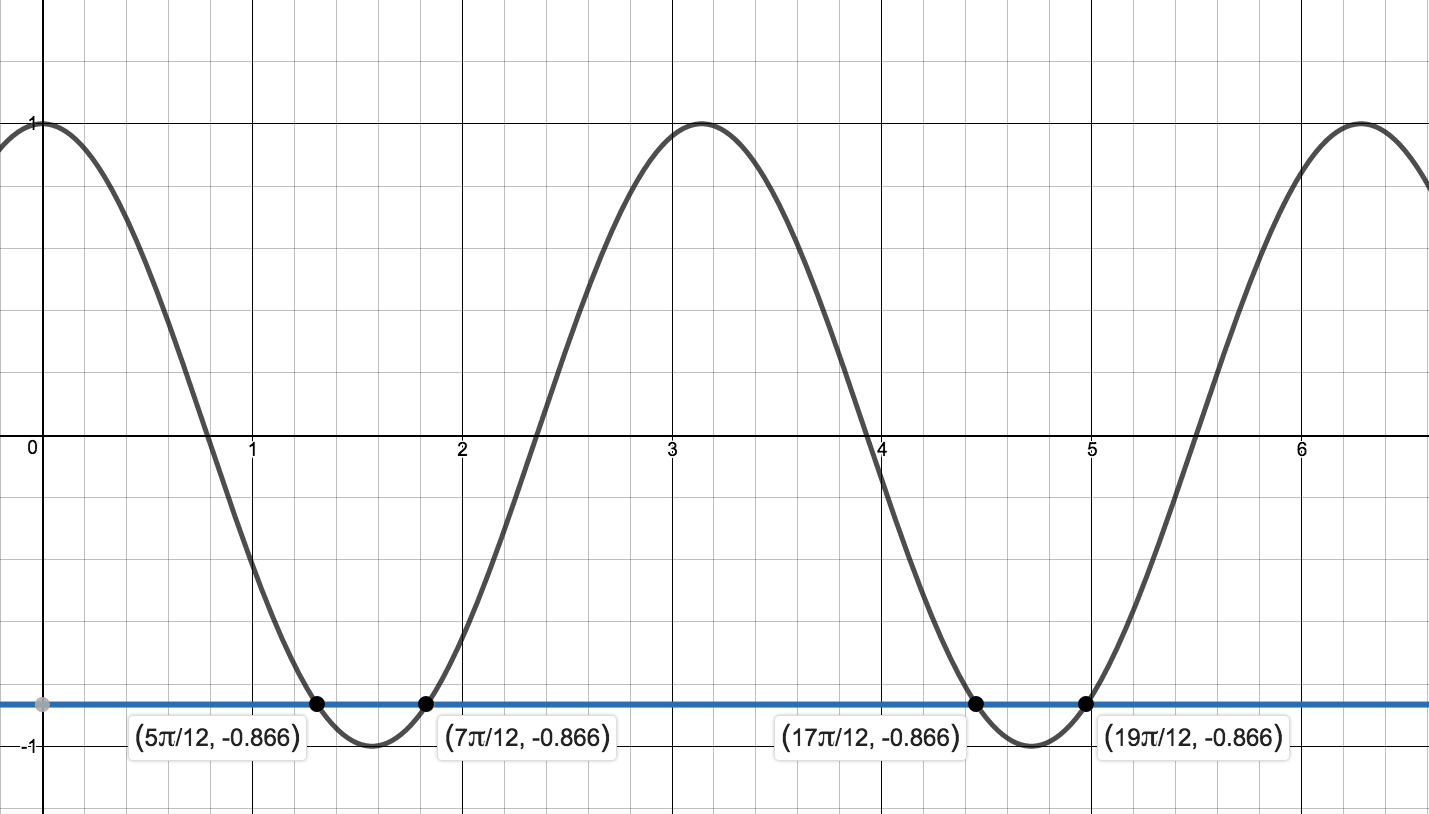
\includegraphics[height=2.25in]{./TrigonometricEquationsandInequalitiesGraphics/TrigEquIneq01.jpg}

{\boldmath $y = \cos(2\theta)$} and $y=-\frac{\sqrt{3}}{2}$

\end{center}


\item  Since this equation has the form $\csc(u) = \sqrt{2}$, we rewrite this as $\sin(u) = \frac{\sqrt{2}}{2}$ and find $u = \frac{\pi}{4} + 2\pi k$ or $u = \frac{3\pi}{4} + 2\pi  k$ for integers $k$.  

\smallskip

Since the argument of cosecant here is $\left(\frac{1}{3}\theta-\pi \right)$,  $\frac{1}{3}\theta-\pi = \frac{\pi}{4} + 2\pi k$ or $\frac{1}{3}\theta - \pi = \frac{3\pi}{4} + 2\pi k$.

\smallskip

To solve $\frac{1}{3} \theta-\pi = \frac{\pi}{4} + 2\pi k$, we first add $\pi$ to both sides to get  $\frac{1}{3} \theta = \frac{\pi}{4} + 2\pi k + \pi$. A common error is to treat the `$2\pi k$' and `$\pi$' terms as `like' terms and try to combine them when they are not.  

\smallskip

We can, however, combine the `$\pi$' and `$\frac{\pi}{4}$' terms to get $\frac{1}{3} \theta = \frac{5\pi}{4} + 2\pi k$.

\smallskip

We now finish by multiplying both sides by $3$ to get  $\theta  = 3 \left( \frac{5\pi}{4} + 2\pi k \right) = \frac{15 \pi}{4} + 6\pi k$, where $k$, as always, runs through the integers.

\smallskip

Solving the other equation, $\frac{1}{3} \theta-\pi = \frac{3\pi}{4} + 2\pi k$ produces $\theta = \frac{21\pi}{4} + 6 \pi k$ for integers $k$. To check the first family of answers, we substitute, combine line terms, and simplify.

\[ \begin{array}{rclr}

\csc\left(\frac{1}{3} \left[ \frac{15\pi}{4} + 6 \pi  k \right] - \pi   \right)  &  = &  \csc\left(\frac{5\pi}{4} + 2\pi k - \pi \right) & \\ [3pt]
																												& =  &   \csc\left(\frac{\pi}{4} + 2\pi k\right) &  \\ [3pt]
																												& =  & \csc\left(\frac{\pi}{4}\right) & \text{(the period of cosecant is $2\pi$)} \\
																												& = & \sqrt{2} & \\
\end{array}\] 



The family $\theta = \frac{21\pi}{4} + 6 \pi  k$ checks similarly. 

\smallskip

 Despite having infinitely many solutions, we find that \textit{none} of them lie in $[0,2\pi)$. 
 
 \smallskip
 
To verify this graphically, we check that $y = \csc\left(\frac{1}{3} \theta -\pi\right)$ and $y =\sqrt{2}$ do not intersect at all over the interval $[0,2\pi)$.


\begin{center}

 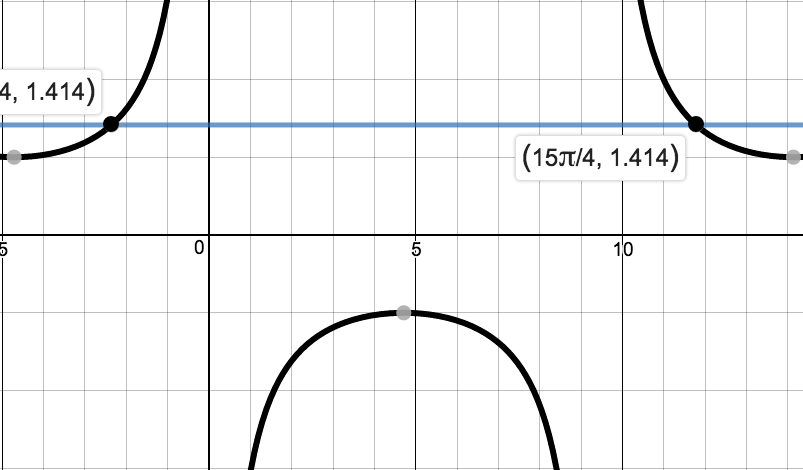
\includegraphics[height=2.25in]{./TrigonometricEquationsandInequalitiesGraphics/TrigEquIneq02.jpg} \\


{\boldmath  $y = \csc\left(\frac{1}{3} \theta -\pi\right)$} and $y =\sqrt{2}$ \\
 


\end{center}

\item  Since $\cot(3t) = 0$ has the form $\cot(u) = 0$, we know $u = \frac{\pi}{2} + \pi k$, so, in this case,  $3t =  \frac{\pi}{2} + \pi k$ for integers $k$.  

\smallskip

Solving for $t$ yields $t = \frac{\pi}{6} + \frac{\pi}{3} k$.  Checking our answers, we get

\[ \begin{array}{rclr}

\cot\left(3\left[ \frac{\pi}{6} + \frac{\pi}{3} k\right]\right)  &  = &  \cot\left(\frac{\pi}{2} + \pi k\right)  & \\ [3pt]
																												& =  &   \cot\left(\frac{\pi}{2}\right) &  \text{(the period of cotangent is $\pi$)} \\ [3pt]
																												& =  & 0 & \\
																								
\end{array}\] 

 As $k$ runs through the integers, we obtain six answers, corresponding to $k=0$ through $k=5$, which lie in $[0, 2\pi)$: $x = \frac{\pi}{6}$, $\frac{\pi}{2}$, $\frac{5\pi}{6}$, $\frac{7\pi}{6}$ , $\frac{3\pi}{2}$ and  $\frac{11\pi}{6}$. 
 
 \smallskip
 
 Graphing $y = \cot(3t)$ and $y=0$ (the $t$-axis), we confirm our result.\footnote{On many calculators, there is no function button for cotangent.  In that case, we would use the quotient identity and graph $y = \frac{\cos(3t)}{\sin(3t)}$ instead.  The reader is invited to see what happens if we would graph $y= \frac{1}{\tan(3t)}$ instead.}
 
 \begin{center}
 
 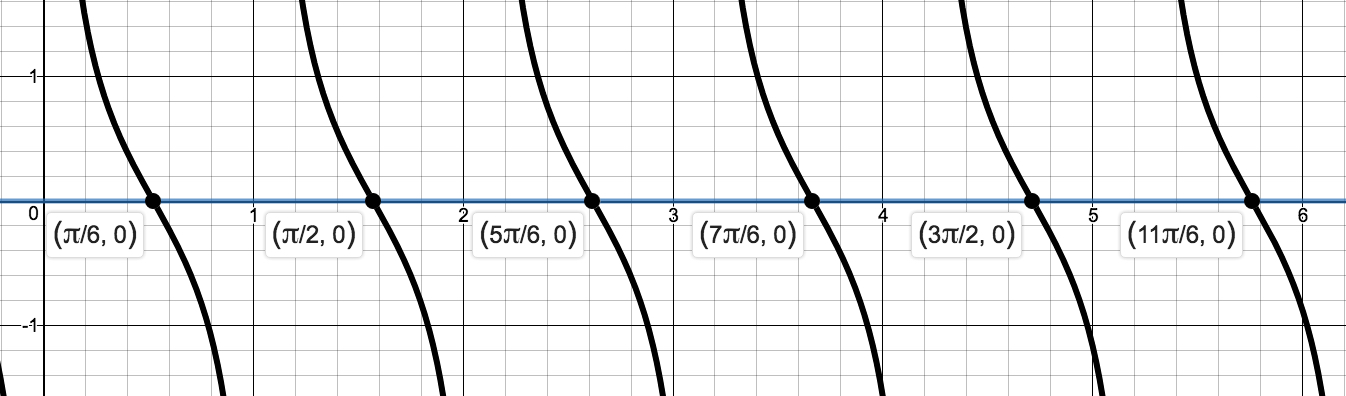
\includegraphics[height=1.75in]{./TrigonometricEquationsandInequalitiesGraphics/TrigEquIneq03.jpg} 
 
 { \boldmath $y = \cot(3t)$}  and $y=0$ 
 
 \end{center}

\item The complication in solving an equation like $\sec^{2}(t) = 4$ comes not from the argument of secant, which is just $t$, but rather, the fact the secant is being squared:  $\sec^{2}(t) = (\sec(t))^2 = 4$.

\smallskip

To get this equation to look like one of the forms listed on page \pageref{trigeqnstrategy1}, we extract square roots to get $\sec(t) = \pm 2$. Converting to cosines, we have  $\cos(t) = \pm \frac{1}{2}$.  

\smallskip

For $\cos(t) = \frac{1}{2}$, we get $t = \frac{\pi}{3} + 2\pi k$ or $t = \frac{5\pi}{3} + 2\pi k$ for integers $k$.  For $\cos(t) = -\frac{1}{2}$, we get $t = \frac{2\pi}{3} + 2\pi k$ or $t = \frac{4\pi}{3} + 2\pi k$ for integers $k$. 

\smallskip

If we take a step back and think of these families of solutions geometrically, we see we are finding the measures of all angles with a reference angle of $\frac{\pi}{3}$.  As a result, these solutions can be combined and we may write our solutions as $t = \frac{\pi}{3} + \pi k$ and $t = \frac{2\pi}{3} + \pi k$ for integers $k$. 

\smallskip

To check the first family of solutions, we note that, depending on the integer $k$,  $\sec\left(\frac{\pi}{3} + \pi k\right)$ doesn't always equal $\sec\left(\frac{\pi}{3}\right)$.  It is true, though,  that for all integers $k$,  $\sec\left(\frac{\pi}{3} + \pi k\right) = \pm \sec\left(\frac{\pi}{3}\right) = \pm 2$.  (Can you show this?)  Hence, checking our first family of solutions gives:


\[ \begin{array}{rclr}

\sec^{2}\left(\frac{\pi}{3} + \pi k\right)  &  = &  \left( \pm \sec\left(\frac{\pi}{3}\right)\right)^2  & \\ [3pt]
																												& =  &   (\pm 2)^2 &  \\ [3pt]
																												& =  & 4 & \\
																								
\end{array}\] 

The check for the family of solutions $t =\frac{2\pi}{3} + \pi k$ is similar. 

\smallskip

 The solutions which lie in $[0,2\pi)$ come from the values $k = 0$ and $k=1$, namely $t = \frac{\pi}{3}$, $\frac{2\pi}{3}$, $\frac{4\pi}{3}$ and $\frac{5\pi}{3}$.  Graphing $y = (\sec(t))^2$ and $y=4$ confirms our results.  

\begin{center}


 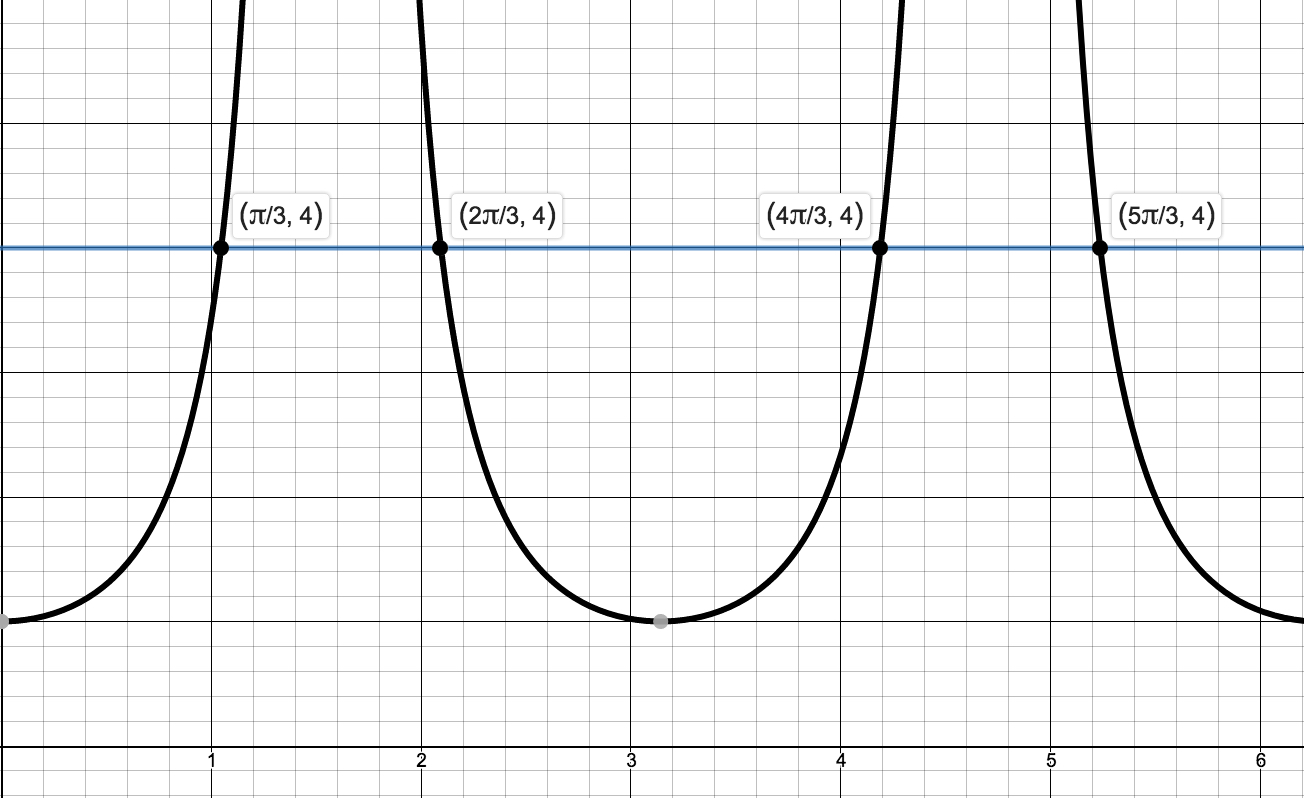
\includegraphics[height=2.25in]{./TrigonometricEquationsandInequalitiesGraphics/TrigEquIneq04.jpg} 

  {\boldmath $y = (\sec(t))^2$} and  $y = 4$  



\end{center}

\item  The equation  $\tan\left(\frac{x}{2}\right) = -3$ has the form $\tan(u) = -3$, whose solution is $u = \arctan(-3) + \pi k$.  

\smallskip

Hence, $\frac{x}{2} = \arctan(-3) + \pi k$, so  $x = 2\arctan(-3) + 2\pi k$ for integers $k$.  To check, we note

\[ \begin{array}{rclr}

\tan\left(\frac{2\arctan(-3) + 2\pi k}{2}\right)  &  = & \tan\left( \arctan(-3) + \pi k \right)  & \\ [3pt]
																												& =  & \tan\left(\arctan(-3) \right) & \text{(the period of tangent is $\pi$)} \\ [3pt]
																												& =  & -3 & (\text{See Theorem } \ref{arctangentcotangentfunctionprops}) \\
																								
\end{array}\] 


 To determine which of our answers lie in the interval $[0,2\pi)$, we first need to get an idea of the value of $2\arctan(-3)$.  While we could easily find an approximation using a calculator,\footnote{Your instructor will let you know if you should abandon the analytic route at this point and use your calculator.} we proceed analytically, as is our custom.
 
 \smallskip
 
To get started, we note that since $-3 < 0$, it  $-\frac{\pi}{2} < \arctan(-3) < 0$.  Hence,  $-\pi < 2\arctan(-3) < 0$.   With regard to our solutions,  $x = 2\arctan(-3) + 2\pi k$, we see for $k = 0$, we get $x = 2\arctan(-3) < 0$, so we discard this answer and all answers $x = 2\arctan(-3) + 2\pi k$ where $k < 0$.  

\smallskip

Next, we turn our attention to $k = 1$ and get $x = 2\arctan(-3) + 2\pi$. Starting with the inequality $-\pi < 2\arctan(-3) < 0$, we add through $2\pi$  and get $\pi < 2\arctan(-3) +2\pi < 2\pi$.  This means $x = 2\arctan(-3) + 2\pi$ lies in $[0,2\pi)$.  

\smallskip

Advancing $k$ to $2$ produces $x = 2\arctan(-3) + 4\pi$. Once again, we get from $-\pi < 2\arctan(-3) < 0$ that $3\pi < 2\arctan(-3) + 4\pi < 4\pi$.  Since this is outside the interval of interest, $[0,2\pi)$,  we discard $x = 2\arctan(-3) + 4\pi$ and all solutions of the form $x = 2\arctan(-3) + 2\pi k$ for $k > 2$.   

\smallskip

Graphically, $y = \tan\left(\frac{x}{2}\right)$ and $y = -3$ intersect only once on $[0,2\pi)$ at $x = 2\arctan(-3) + 2\pi\approx 3.785$.

\smallskip

\begin{center}


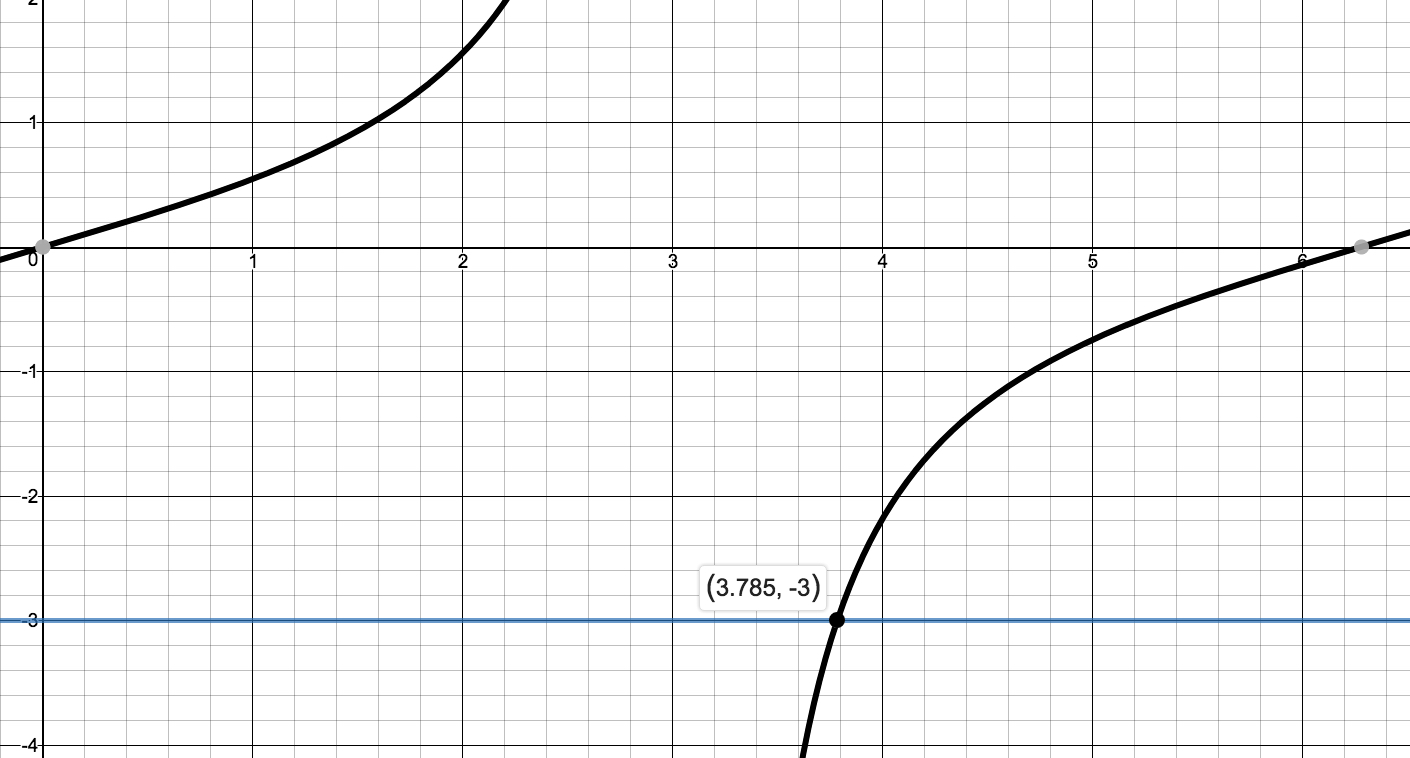
\includegraphics[height=2.25in]{./TrigonometricEquationsandInequalitiesGraphics/TrigEquIneq05.jpg}

{ \boldmath $y = \tan\left(\frac{x}{2}\right)$} and  $y = -3$ 

\end{center}

\item To solve $\sin(2x) = 0.87$, we first note that it has the form $\sin(u) = 0.87$, which has the family of solutions $u = \arcsin(0.87) + 2\pi k$ or $u =\pi -  \arcsin(0.87) + 2\pi k$ for integers $k$. 

\smallskip

Since the argument of sine here is $2x$, we get $2x = \arcsin(0.87) + 2\pi k$ or $2x =\pi -  \arcsin(0.87) + 2\pi k$ which gives $x = \frac{1}{2} \arcsin(0.87) + \pi k$ or $x =\frac{\pi}{2} -  \frac{1}{2}\arcsin(0.87) + \pi k$ for integers $k$.  To check,

\[ \begin{array}{rclr}

\sin\left(2\left[\frac{1}{2} \arcsin(0.87) + \pi k\right]\right)  &  = & \sin\left(\arcsin(0.87) + 2\pi k\right)  & \\ [3pt]
																													& =  & \sin\left(\arcsin(0.87)\right) & \text{(the period of sine is $2\pi$)} \\ [3pt]
																												& =  & 0.87& (\text{See Theorem } \ref{arccosinesinefunctionprops})\\
																								
\end{array}\] 


For the family $x =\frac{\pi}{2} -  \frac{1}{2}\arcsin(0.87) + \pi k$ , we get

\[ \begin{array}{rclr}

\sin\left(2\left[\frac{\pi}{2} - \frac{1}{2} \arcsin(0.87) + \pi k\right]\right)  &  = & \sin\left(\pi - \arcsin(0.87) + 2\pi k\right) & \\ [3pt]
																												& =  & \sin\left(\pi - \arcsin(0.87)\right) & \text{(the period of sine is $2\pi$)} \\ [3pt]
																												& =  & \sin\left(\arcsin(0.87)\right) & \text{($\sin(\pi - t) = \sin(t)$)} \\ [3pt]
																												& =  & 0.87& (\text{See Theorem } \ref{arccosinesinefunctionprops}) \\
																								
\end{array}\] 

To determine which of these solutions lie in $[0,2\pi)$, we first need to get an idea of the value of $x=\frac{1}{2} \arcsin(0.87)$.  Once again, we could use the calculator, but we adopt an analytic route here.  

\smallskip

By definition, $0 < \arcsin(0.87) < \frac{\pi}{2}$ so that multiplying through by $\frac{1}{2}$ gives us $0 < \frac{1}{2} \arcsin(0.87) < \frac{\pi}{4}$.  

\smallskip

Starting with the family of solutions $x = \frac{1}{2} \arcsin(0.87) + \pi k$, we use the same kind of arguments as in our solution to number \ref{arctanin02pi} above and find only the solutions corresponding to $k =0$ and $k=1$ lie in $[0,2\pi)$:  $x = \frac{1}{2} \arcsin(0.87)$ and $x = \frac{1}{2} \arcsin(0.87) + \pi$. 

\smallskip

 Next, we move to the family $x =\frac{\pi}{2} -  \frac{1}{2}\arcsin(0.87) + \pi k$ for integers $k$. Here, we need to get a better estimate of $\frac{\pi}{2} - \frac{1}{2} \arcsin(0.87)$.  From the inequality $0 < \frac{1}{2}\arcsin(0.87) < \frac{\pi}{4}$, we first multiply through by $-1$ and then add $\frac{\pi}{2}$ to get $\frac{\pi}{2} > \frac{\pi}{2} -\frac{1}{2} \arcsin(0.87) >  \frac{\pi}{4}$, or $\frac{\pi}{4} < \frac{\pi}{2} -\frac{1}{2} \arcsin(0.87) < \frac{\pi}{2}$.  
 
 \smallskip
 
 Proceeding with the usual arguments, we find the only solutions which lie in $[0,2\pi)$ correspond to $k = 0$ and $k=1$, namely $x =\frac{\pi}{2} -  \frac{1}{2}\arcsin(0.87)$ and  $x = \frac{3\pi}{2} - \frac{1}{2}\arcsin(0.87)$. 
 
 \smallskip
 
All told, we have found four solutions to $\sin(2x) = 0.87$ in $[0,2\pi)$:  $x =\frac{1}{2} \arcsin(0.87) \approx 0.528$, $x=\frac{1}{2} \arcsin(0.87) + \pi \approx 3.669$, $x =\frac{\pi}{2} -  \frac{1}{2}\arcsin(0.87) \approx 1.043$ and  $x = \frac{3\pi}{2} - \frac{1}{2}\arcsin(0.87) \approx 4.185$. By graphing $y = \sin(2x)$ and $y = 0.87$, we confirm our results.



\begin{center}


  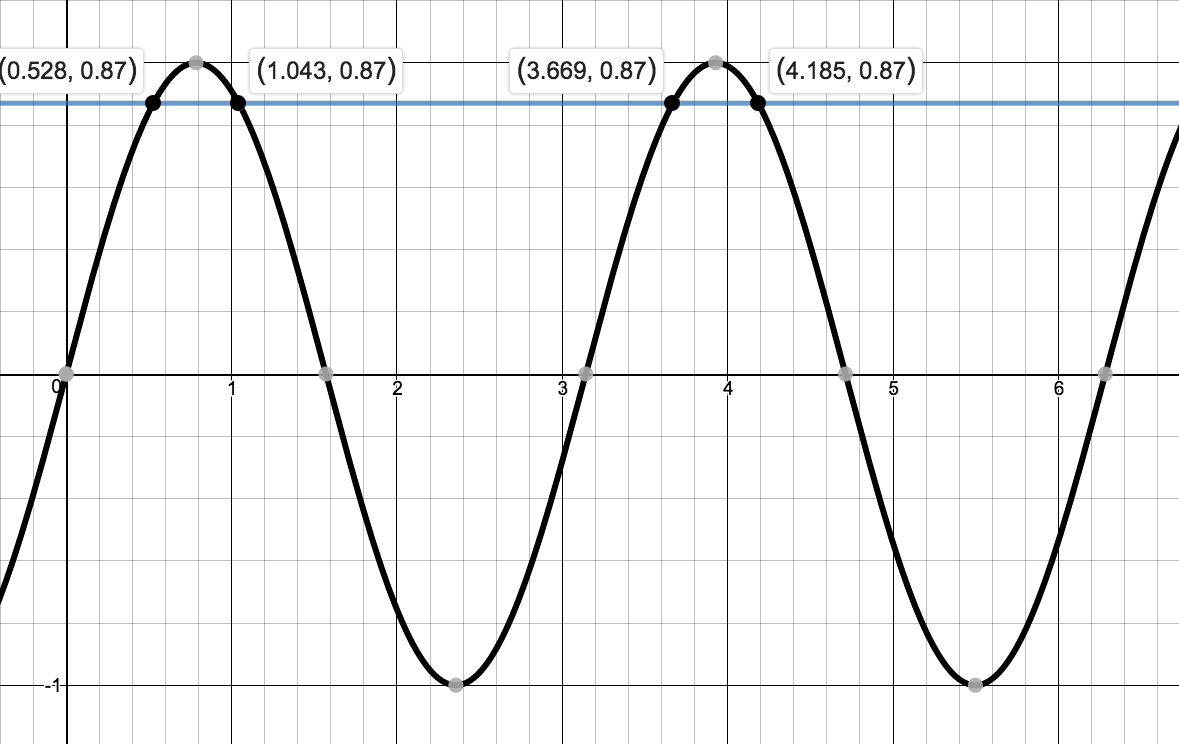
\includegraphics[height=2.25in]{./TrigonometricEquationsandInequalitiesGraphics/TrigEquIneq06.jpg} 

{\boldmath $y = \sin(2x)$} and  $y = 0.87$


\end{center} 

\end{enumerate}

\vspace*{-.3in} \qed

\end{example}


If one looks closely at the equations and solutions in Example \ref{TrigEqnEx1}, an interesting relationship evolves between the frequency of the circular function involved in the equation and how many solutions one can expect in the interval $[0, 2\pi)$.   This relationship is explored in Exercise \ref{frequencynumberconnection}.

\smallskip

Each of the problems in Example \ref{TrigEqnEx1} featured one circular function.  If an equation involves two different circular functions or if the equation contains the same circular function but with different arguments, we will need to employ identities and Algebra to reduce the equation to the same form as those given on page  \pageref{trigeqnstrategy1}.  We demonstrate these techniques in the following example.
 
\begin{example} \label{TrigEqIdEx1}  Solve the following equations and list the solutions which lie in the interval $[0,2\pi)$.  Verify your solutions on $[0,2\pi)$ graphically.

\begin{multicols}{2}

\begin{enumerate}

\item  $3\sin^{3}(\theta) = \sin^{2}(\theta)$
\item $\sec^{2}(\theta) = \tan(\theta) + 3$

\setcounter{HW}{\value{enumi}}

\end{enumerate}

\end{multicols}

\begin{multicols}{2}

\begin{enumerate}

\setcounter{enumi}{\value{HW}}

\item   $\cos(2t) = 3\cos(t) - 2$
\item  $\cos(3t) = 2- \cos(t)$

\setcounter{HW}{\value{enumi}}

\end{enumerate}

\end{multicols}

\begin{multicols}{2}

\begin{enumerate}

\setcounter{enumi}{\value{HW}}

\item  $\cos(3x) = \cos(5x)$
\item $\sin(2x) =\sqrt{3} \cos(x)$

\setcounter{HW}{\value{enumi}}

\end{enumerate}

\end{multicols}

\begin{multicols}{2}

\begin{enumerate}

\setcounter{enumi}{\value{HW}}

\item  $\sin(x)\cos\left(\frac{x}{2}\right) + \cos(x)\sin\left(\frac{x}{2}\right) = 1$
\item  $\cos(x) - \sqrt{3} \sin(x) = 2$

\end{enumerate}
 
\end{multicols}

\newpage

{\bf Solution.}

\begin{enumerate}

\item One approach to solving  $3\sin^{3}(\theta) = \sin^{2}(\theta)$ begins with dividing both sides by $\sin^{2}(\theta)$.  Doing so, however, assumes that $\sin^{2}(\theta) \neq 0$ which means we risk losing solutions.  

\smallskip

Instead, we take a cue from Chapter \ref{PolynomialFunctions} (since what we have here is a polynomial equation in terms of $\sin(\theta)$) and gather all the nonzero terms on one side and factor:
\[ \begin{array}{rclr}

3\sin^{3}(\theta) & = &  \sin^{2}(\theta) & \\
3\sin^{3}(\theta) -  \sin^{2}(\theta) & = & 0 &  \\
\sin^{2}(\theta) (3 \sin(\theta) - 1) & = & 0 & \text{Factor out $\sin^{2}(\theta)$ from both terms.} \\ \end{array} \]

We get $\sin^{2}(\theta) = 0$ or $3\sin(\theta) - 1 = 0$, so $\sin(\theta) = 0$ or $\sin(\theta) = \frac{1}{3}$.  The solution to $\sin(\theta) = 0$ is $\theta = \pi k$, with $\theta = 0$ and $\theta = \pi$ being the two solutions which lie in $[0,2\pi)$.  

\smallskip

To solve $\sin(\theta) = \frac{1}{3}$, we use the arcsine function to get $\theta = \arcsin\left(\frac{1}{3}\right) + 2\pi k$ or $\theta = \pi - \arcsin\left(\frac{1}{3}\right) + 2\pi k$ for integers $k$. We find the two solutions here which lie in $[0,2\pi)$ to be $\theta = \arcsin\left(\frac{1}{3}\right) \approx 0.34$ and $\theta = \pi - \arcsin\left(\frac{1}{3}\right) \approx 2.80$.  

\smallskip

To check graphically, we plot $y = 3(\sin(\theta))^3$ and $y = (\sin(\theta))^2$ and find the  $\theta$-coordinates of the intersection points of these two curves.\footnote{Note that we do \textit{not} list  $\theta = 2\pi$ as part of the solution over the interval $[0,2\pi)$ since $2\pi$ is not in $[0, 2\pi)$.}  (Some extra zooming may be required near $\theta=0$ and $\theta=\pi$ to verify that these two curves do in fact intersect four times.)  

\smallskip



\begin{center}


  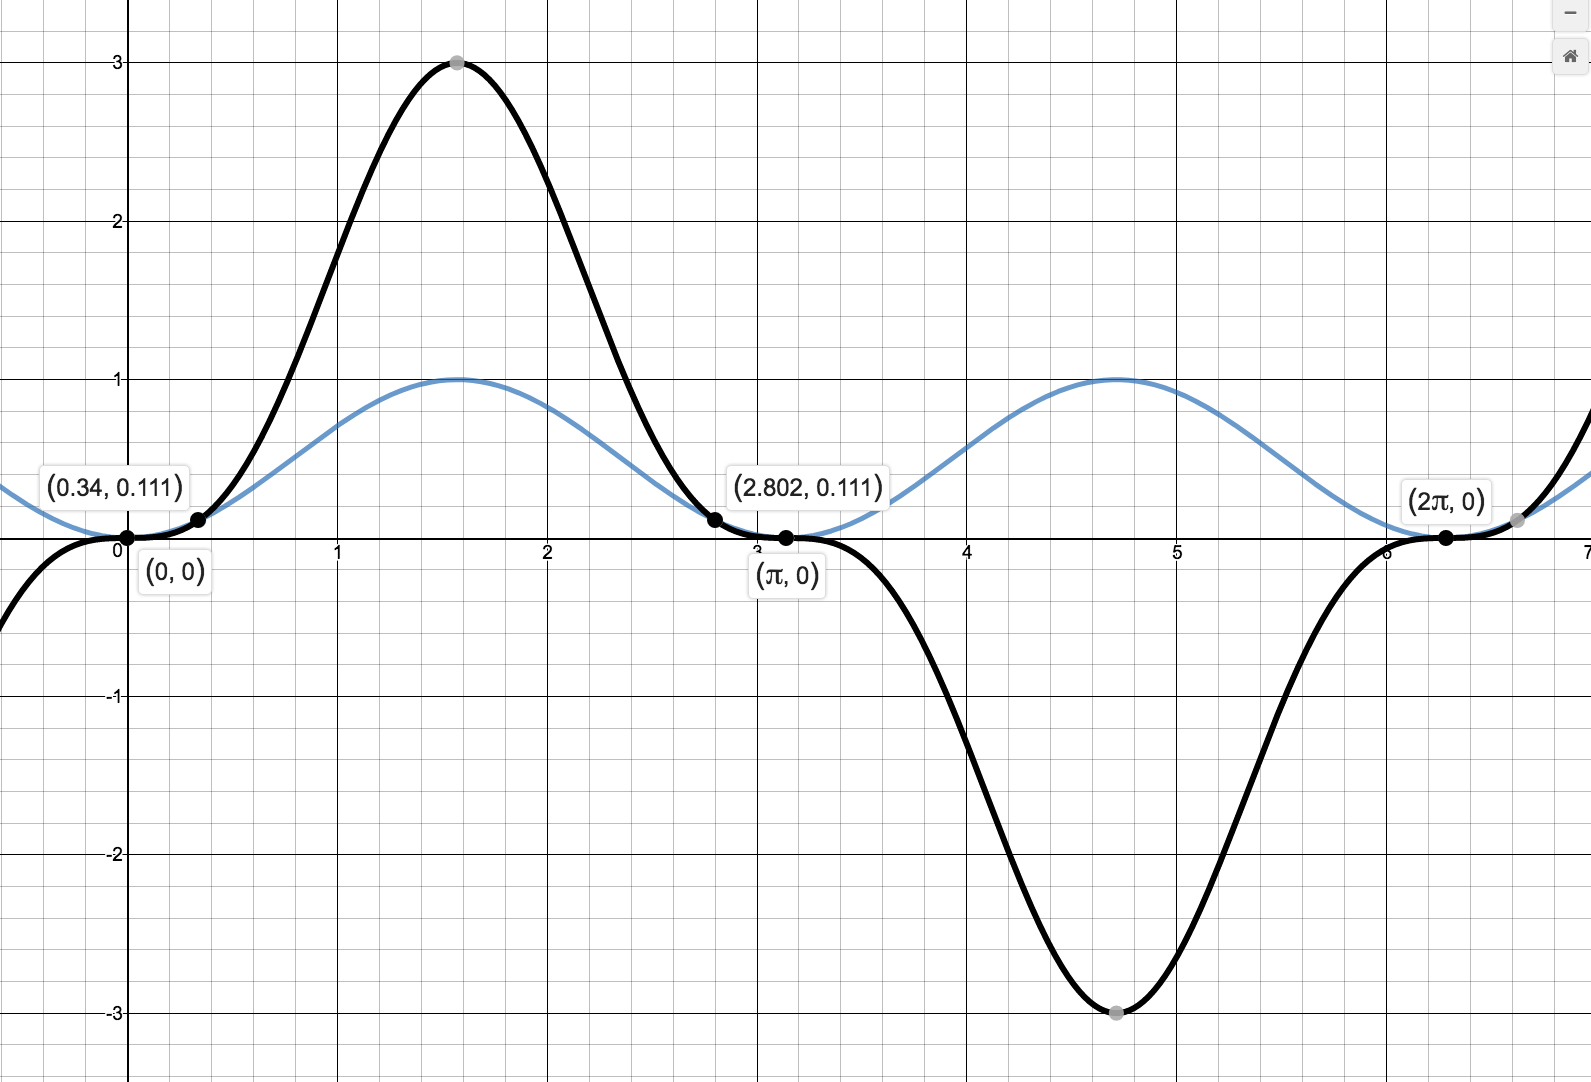
\includegraphics[height=2.25in]{./TrigonometricEquationsandInequalitiesGraphics/TrigEquIneq07.jpg} 

{\boldmath $y = 3(\sin(\theta))^3$} and  $y = (\sin(\theta))^2$


\end{center} 

\item We see immediately in the equation $\sec^{2}(\theta) = \tan(\theta) + 3$ that there are two different circular functions present, so we look for an identity to express both sides in terms of the same function.  

\smallskip

We use the Pythagorean Identity $\sec^{2}(\theta) = 1 + \tan^{2}(\theta)$ to exchange $\sec^{2}(\theta)$  for tangents.  What results is a `quadratic in disguise:'\footnote{See Section \ref{AppQuadEqus} for a review of this concept.}

\[ \begin{array}{rclr}

\sec^{2}(\theta) &  = & \tan(\theta) + 3 & \\
1 + \tan^{2}(\theta) & = & \tan(\theta) + 3& \text{(Since $\sec^{2}(\theta) = 1 + \tan^{2}(\theta)$.)} \\
\tan^{2}(\theta) - \tan(\theta) -2 & = & 0 & \\
u^2 - u - 2 & = & 0 & \text{Let $u = \tan(\theta)$.} \\
(u + 1)(u - 2) & = & 0 & \\ \end{array} \]

This gives $u = -1$ or $u = 2$.  Since $u = \tan(\theta)$, we have $\tan(\theta) = -1$ or $\tan(\theta) = 2$. 

\smallskip

From $\tan(\theta) = -1$, we get $\theta = -\frac{\pi}{4} + \pi k$ for integers $k$.  To solve $\tan(\theta) = 2$, we employ the arctangent function and get $\theta = \arctan(2) + \pi k$ for integers $k$.  

\smallskip

From the first set of solutions, we get $\theta = \frac{3\pi}{4}$ and $\theta = \frac{7\pi}{4}$ as our answers which lie in $[0,2\pi)$.  

\smallskip

Using the same sort of argument we saw in Example \ref{TrigEqnEx1},   we get  $\theta=\arctan(2) \approx 1.107$ and $\theta = \pi + \arctan(2) \approx 4.249$ as answers from our second set of solutions which lie in $[0,2\pi)$.  

\smallskip

We verify our solutions below graphically.  

\begin{center}

 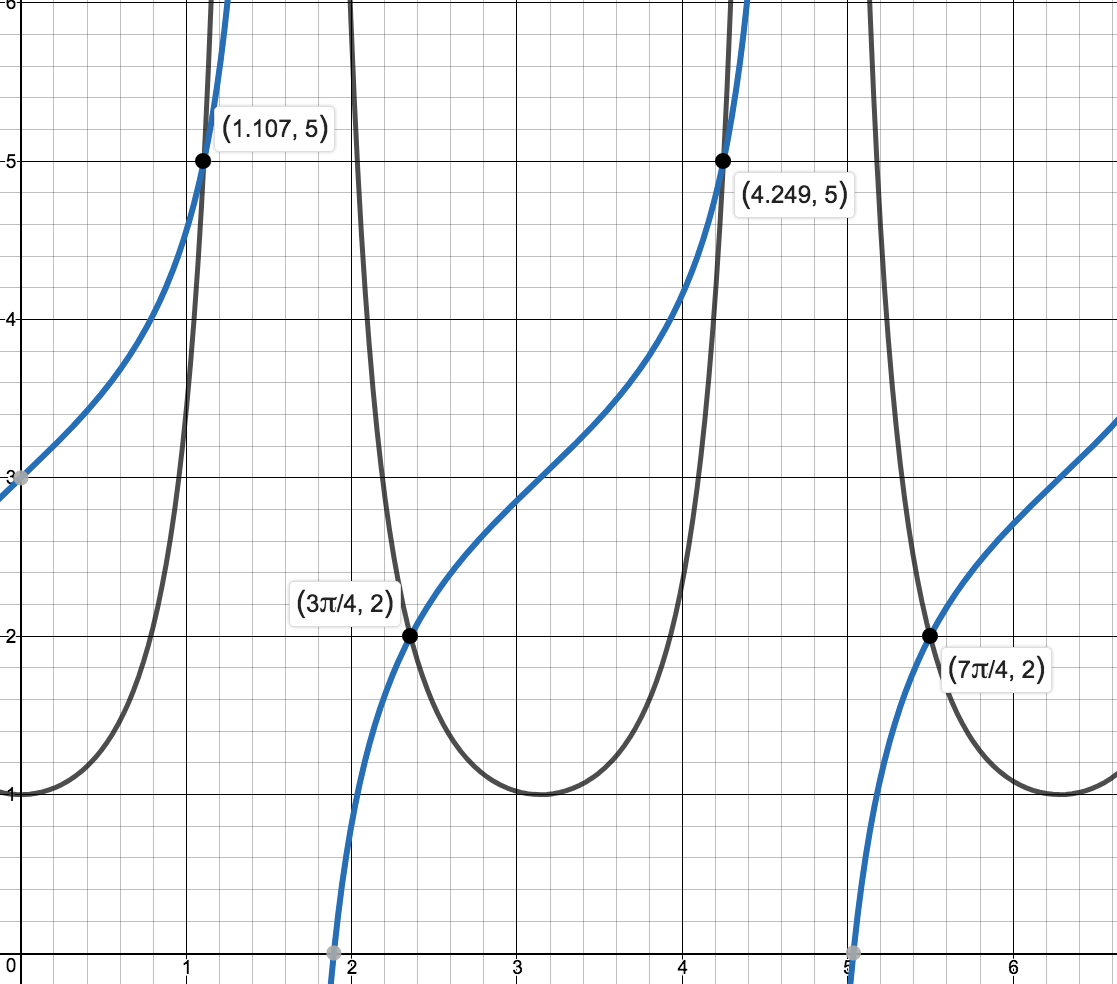
\includegraphics[height=2.25in]{./TrigonometricEquationsandInequalitiesGraphics/TrigEquIneq08.jpg} \\

{ \boldmath  $y =(\sec(\theta))^2$} and $y = \tan(\theta) + 3$  
 
\end{center}

\item  The good news is that in the equation $\cos(2t) = 3\cos(t) - 2$, we have the same circular function, cosine,  throughout.  The bad news is that we have different arguments, $2t$ and $t$.  

\smallskip

Using the double angle identity $\cos(2t) = 2\cos^{2}(t) - 1$ results in another quadratic in disguise:'

\[ \begin{array}{rclr}

\cos(2t) & = & 3\cos(t) - 2 & \\
2\cos^{2}(t) -1 & = & 3\cos(t) -2 & \text{(Since $\cos(2t) = 2\cos^{2}(t) -1$.)} \\
2\cos^{2}(t) - 3\cos(t) +1 & = & 0 & \\
2 u^2 - 3 u + 1 & = & 0 & \text{Let $u = \cos(t)$.}\\
(2u - 1)(u - 1) & = & 0 & \\ \end{array} \]

We get $u = \frac{1}{2}$ or $u = 1$, so   $\cos(t) = \frac{1}{2}$ or $\cos(t) = 1$. Solving  $\cos(t) = \frac{1}{2}$, we get $t = \frac{\pi}{3} + 2\pi k$ or $t = \frac{5\pi}{3} + 2\pi k$ for integers $k$.  From $\cos(t) = 1$, we get $t = 2\pi k$ for integers $k$.  

\smallskip

The answers which lie in $[0,2\pi)$ are $t =0$,  $\frac{\pi}{3}$, and $\frac{5\pi}{3}$.  Graphing $y = \cos(2t)$ and $y = 3\cos(t) - 2$, we find that the curves intersect in three places on $[0,2\pi)$ and confirm our results.

\begin{center}

 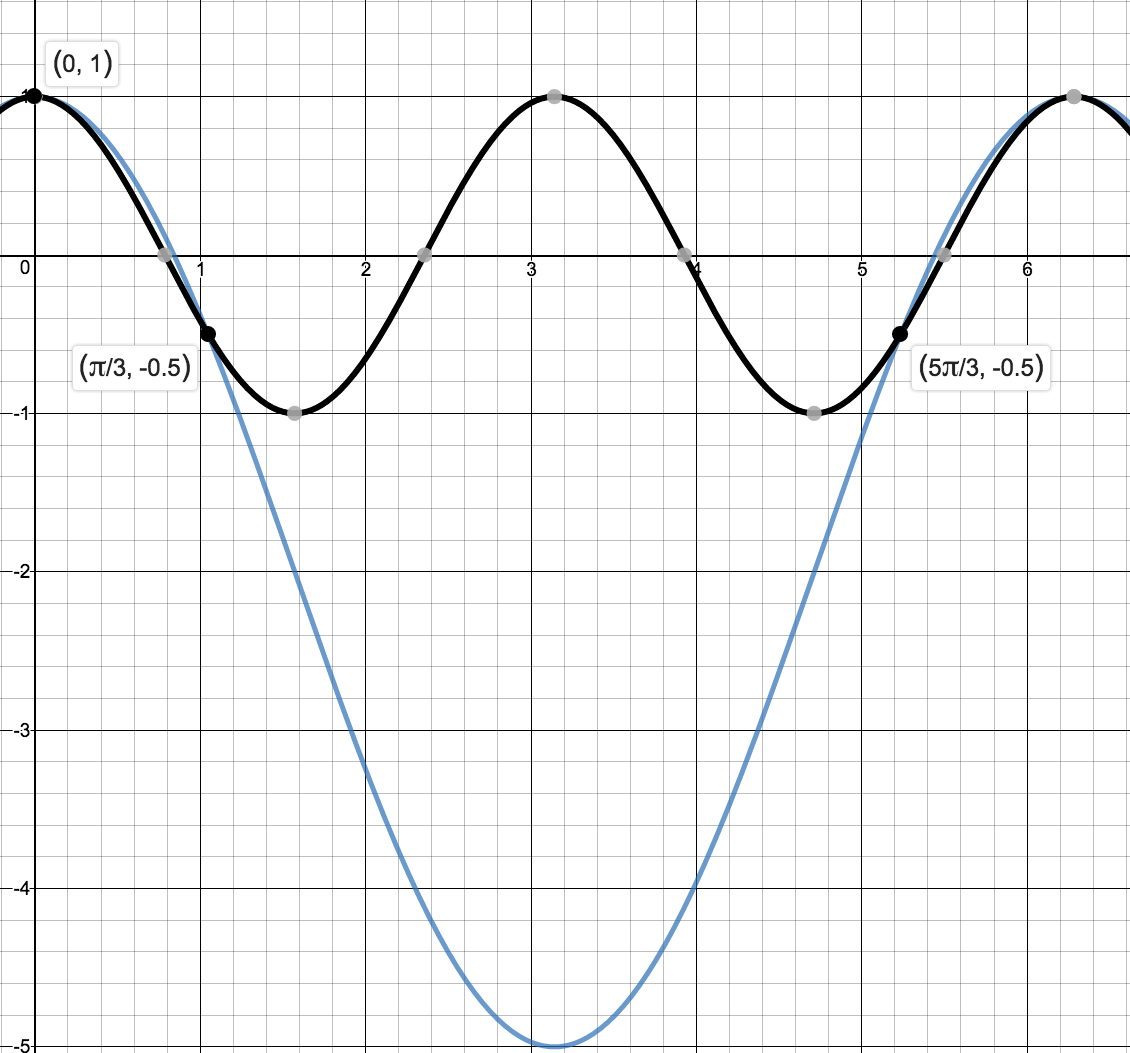
\includegraphics[height=2.25in]{./TrigonometricEquationsandInequalitiesGraphics/TrigEquIneq09.jpg}

{ \boldmath  $y =\cos(2t)$} and $y = 3 \cos(t)  - 2$  
 
\end{center}



\item  To solve $\cos(3t) = 2- \cos(t)$, we take a cue from the previous problem and look for an identity to rewrite $\cos(3t)$ in terms of $\cos(t)$.

\smallskip

  From Example \ref{doubleangleex}, number \ref{cosinepolynomial}, we know that $\cos(3t) = 4\cos^{3}(t) - 3\cos(t)$.  This transforms the equation into a polynomial in terms of $\cos(t)$.


\[ \begin{array}{rclr}

\cos(3t) & = &2- \cos(t) & \\
4\cos^{3}(t) - 3\cos(t) & = & 2- \cos(t) & \\
2\cos^{3}(t) - 2\cos(t) -2  & = & 0 & \\
4 u^3 - 2 u -2  & = & 0 & \text{Let $u = \cos(t)$.} \\ \end{array} \]

Using what we know from Chapter \ref{PolynomialFunctions}, we factor $4u^3-2u-2$ as $(u-1)\left(4u^2+4u+2\right)$ and set each factor equal to $0$.  

\smallskip

We get either $u-1 = 0$ or  $4u^2+2u+2=0$, and since the discriminant of the latter is negative, the only real solution to $4u^3-2u-2=0$ is $u = 1$.  


\smallskip

Since $u = \cos(t)$, we get $\cos(t) = 1$, so $t = 2\pi k$ for integers $k$.  The only solution which lies in $[0,2\pi)$ is $t = 0$.  Our graph below confirms this.

\begin{center}

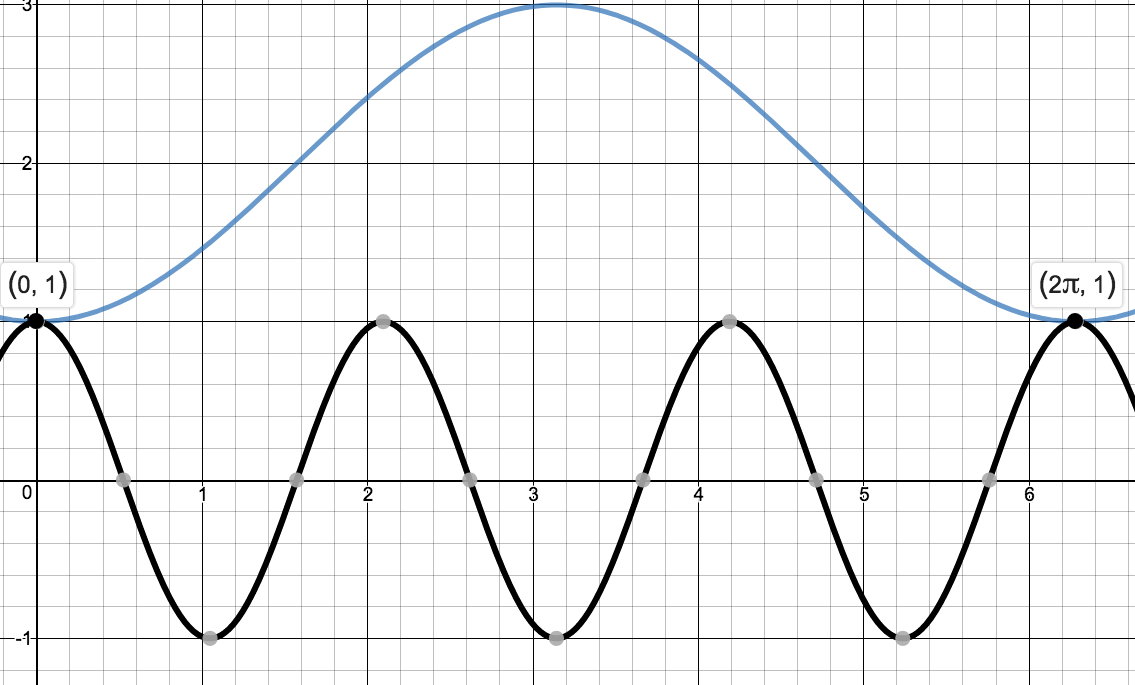
\includegraphics[height=2.25in]{./TrigonometricEquationsandInequalitiesGraphics/TrigEquIneq10.jpg} 

{\boldmath $y = \cos(3t)$} and  $y = 2- \cos(t)$
\end{center}


\item  While we could approach solving the equation $\cos(3x) = \cos(5x)$ in the same manner as we did the previous two problems, we choose instead to showcase the utility of the Sum to Product Identities.\footnote{We invite the reader to try the `polynomial approach' used in the previous problem to see what difficulties are encountered.}

\smallskip

From $\cos(3x) = \cos(5x)$, we get $\cos(5x) - \cos(3x) = 0$, and it is the presence of $0$ on the right hand side that indicates a switch to a product would be a good move.\footnote{Since a \textit{product} equalling zero means, necessarily, one or both \textit{factors} is $0$.  See page \ref{propertiesofzero}.}

\smallskip

 Using Theorem \ref{sumtoproduct}, we rewrite $\cos(5x) - \cos(3x)$  as $- 2 \sin\left( \frac{5x + 3x}{2}\right)\sin\left( \frac{5x - 3x}{2}\right) = -2 \sin(4x)\sin(x)$.  Hence, our original equation $\cos(3x) = \cos(5x)$ is equivalent to $-2 \sin(4x) \sin(x) = 0$.  
 
 \smallskip
 
From $-2 \sin(4x) \sin(x) = 0$, we get either  $\sin(4x) = 0$ or $\sin(x)$ = 0. Solving $\sin(4x) = 0$ gives $x = \frac{\pi}{4} k$ for integers $k$, and the solution to $\sin(x) = 0$ is $x = \pi k$ for integers $k$.  

\smallskip

The second set of solutions is contained in the first set of solutions,\footnote{As always, when in doubt, write it out!} so our final solution to $\cos(5x) = \cos(3x)$ is $x = \frac{\pi}{4} k$ for integers $k$.  

\smallskip

There are eight of these answers which lie in $[0,2\pi)$:  $x = 0$, $\frac{\pi}{4}$, $\frac{\pi}{2}$, $\frac{3\pi}{4}$, $\pi$, $\frac{5\pi}{4}$, $\frac{3\pi}{2}$ and $\frac{7\pi}{4}$.  Our plot of the graphs of $y = \cos(3x)$ and $y = \cos(5x)$ below (after some careful zooming) bears this out. 

\begin{center}

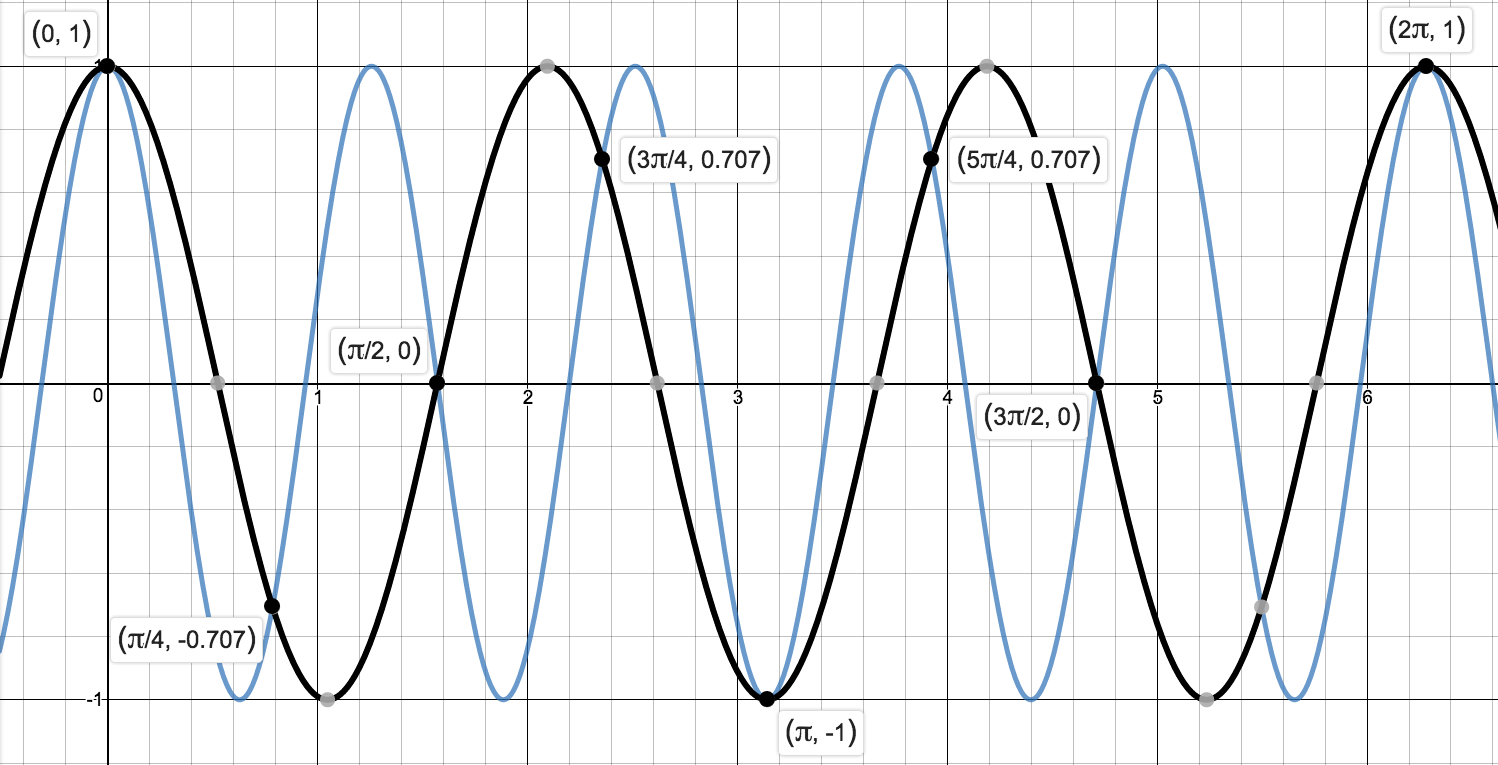
\includegraphics[height=2.25in]{./TrigonometricEquationsandInequalitiesGraphics/TrigEquIneq11.jpg} 

{\boldmath $y = \cos(3x)$} and  $y = cos(5x)$

\end{center}

\item  In the equation   $\sin(2x) =\sqrt{3} \cos(x)$, we not only  have different circular functions involved,  but we also have different arguments to contend with.  

\smallskip

Using the double angle identity $\sin(2x) = 2 \sin(x) \cos(x)$ makes all of the arguments the same and we proceed to gather all of the nonzero terms on one side of the equation and factor.

\[ \begin{array}{rclr}

\sin(2x) & = & \sqrt{3} \cos(x) & \\
2 \sin(x) \cos(x) & = & \sqrt{3} \cos(x)  & \text{(Since $\sin(2x) = 2\sin(x) \cos(x)$.)} \\
2\sin(x) \cos(x) - \sqrt{3} \cos(x) & = & 0 & \\
\cos(x) (2 \sin(x) - \sqrt{3}) & = & 0 & \\ \end{array} \]

We get $\cos(x) = 0$ or $\sin(x) = \frac{\sqrt{3}}{2}$. From $\cos(x) = 0$, we obtain $x = \frac{\pi}{2} + \pi k$ for integers $k$. From $\sin(x) = \frac{\sqrt{3}}{2}$, we get $x = \frac{\pi}{3} + 2\pi k$ or $x = \frac{2\pi}{3} + 2\pi k$ for integers $k$.  

\smallskip

The answers which lie in $[0,2\pi)$ are $x = \frac{\pi}{2}$, $\frac{3\pi}{2}$, $\frac{\pi}{3}$ and $\frac{2\pi}{3}$, as verified graphically below.

\begin{center}

 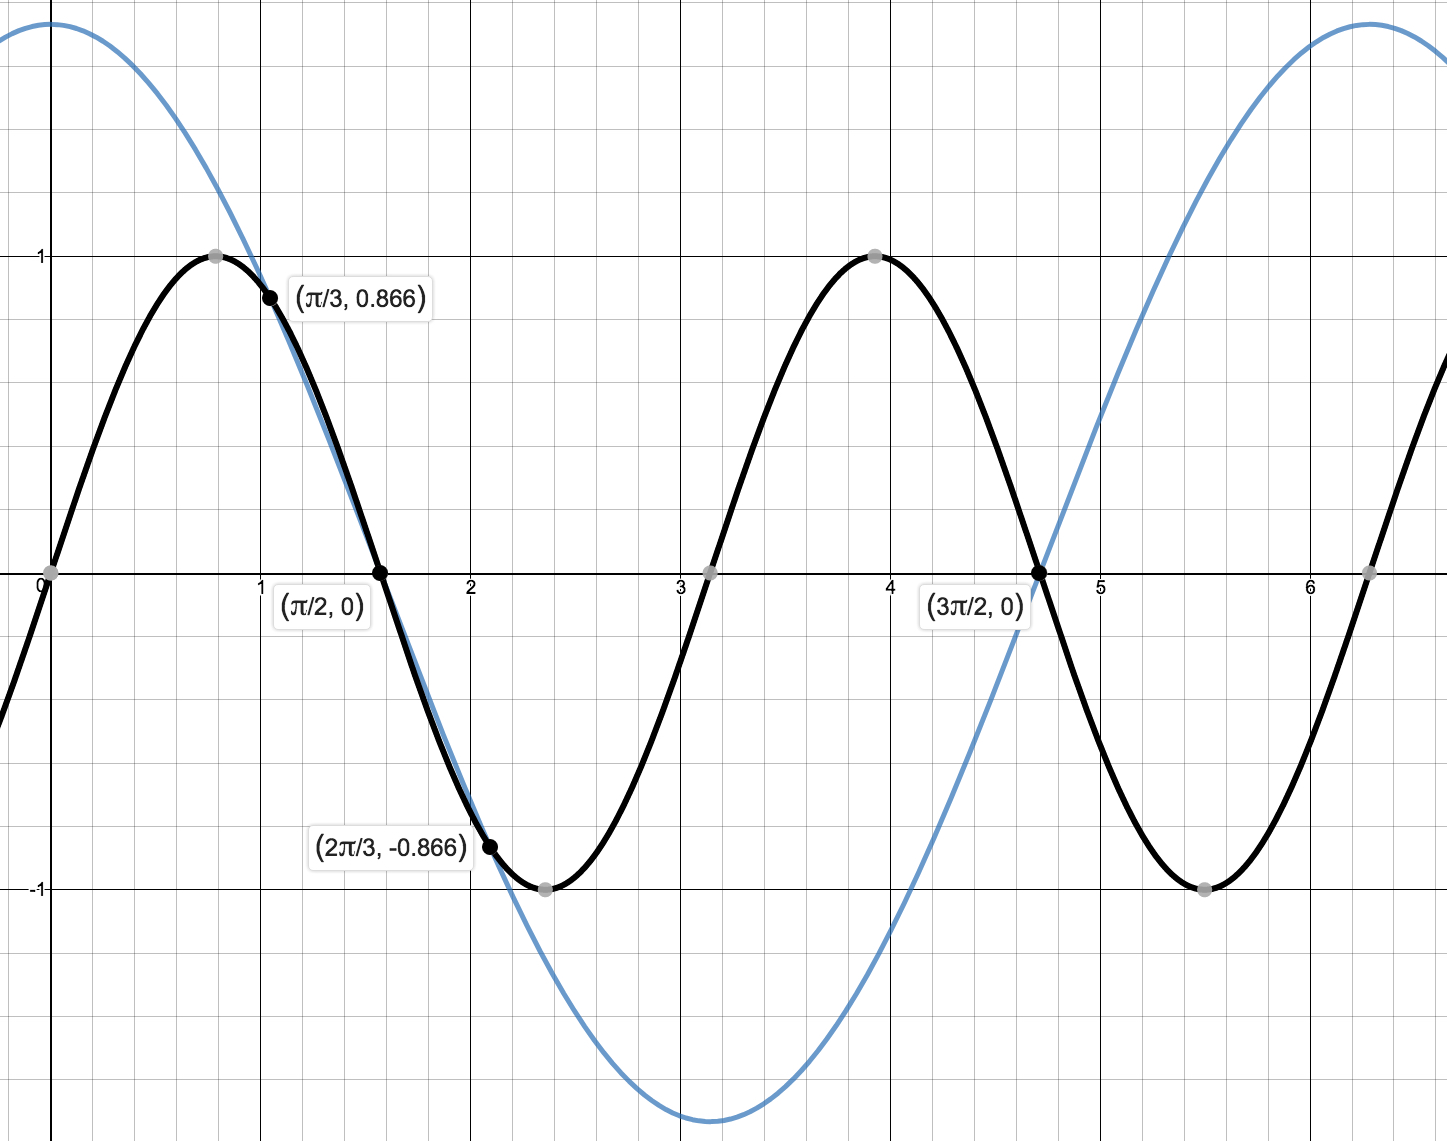
\includegraphics[height=2.25in]{./TrigonometricEquationsandInequalitiesGraphics/TrigEquIneq12.jpg} 

{\boldmath $y = \sin(2x)$} and  $y = \sqrt{3} \cos(x)$  
 
\end{center}

\item Unlike the previous problem, there seems to be no quick way to get the circular functions or their arguments to match in the equation $\sin(x)\cos\left(\frac{x}{2}\right) + \cos(x)\sin\left(\frac{x}{2}\right) = 1$. 

\smallskip

 If we stare at it long enough, however,  we realize that the left hand side is the expanded form of the sum formula for $\sin\left(x + \frac{x}{2}\right)$.  Hence, our original equation is equivalent to  $\sin\left(\frac{3}{2} x\right) = 1$.  
 
 \smallskip
 
 Solving, we find $x = \frac{\pi}{3} + \frac{4\pi}{3} k$ for integers $k$.  Two of these solutions lie in $[0,2\pi)$: $x = \frac{\pi}{3}$ and $x = \frac{5\pi}{3}$. Graphing $y = \sin(x)\cos\left(\frac{x}{2}\right) + \cos(x)\sin\left(\frac{x}{2}\right)$ and $y = 1$ validates our solutions.
 
 
\begin{center}

 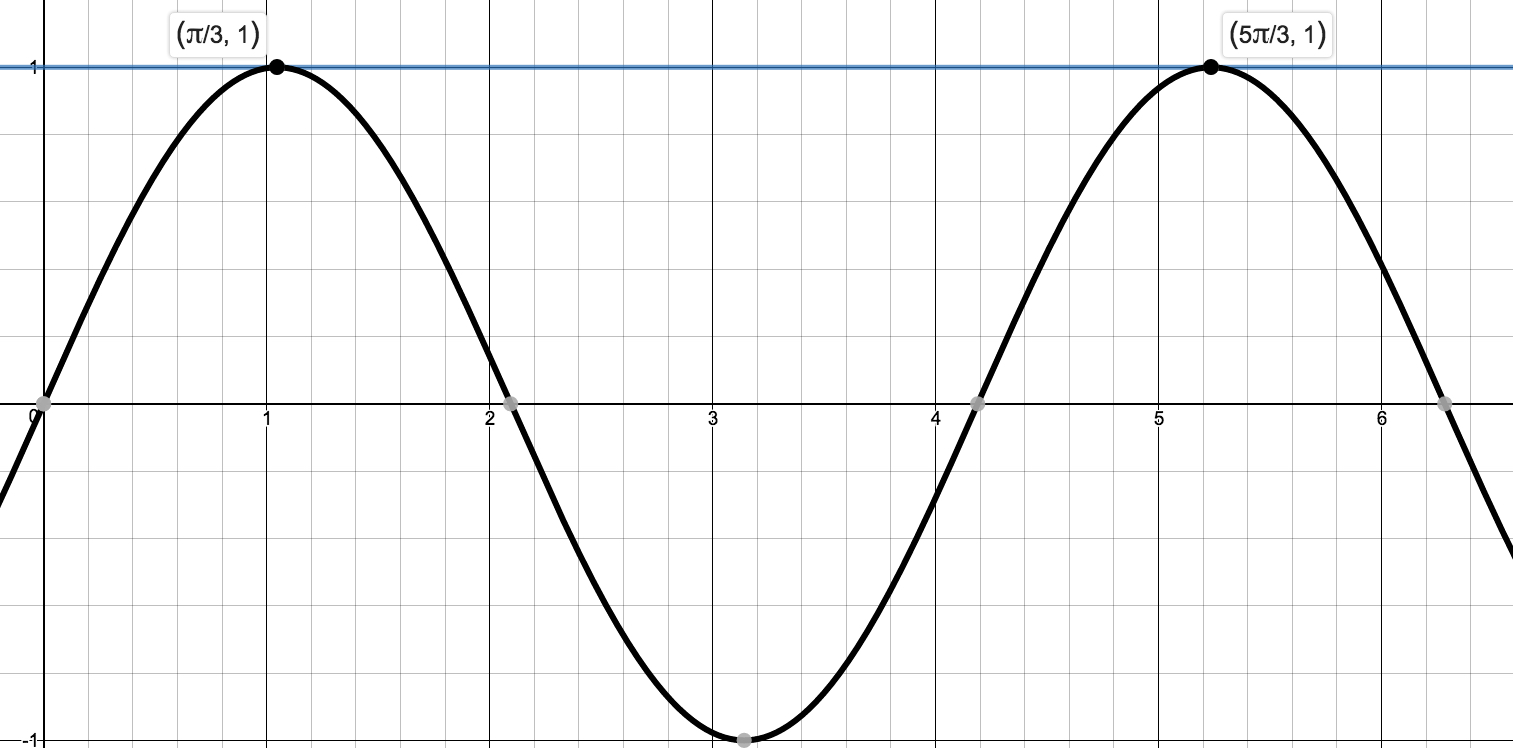
\includegraphics[height=2.25in]{./TrigonometricEquationsandInequalitiesGraphics/TrigEquIneq13.jpg} 

{\boldmath $y = \sin(x)\cos\left(\frac{x}{2}\right) + \cos(x)\sin\left(\frac{x}{2}\right)$} and $y = 1$
 
\end{center}


\item  With the absence of double angles or squares, there doesn't seem to be much we can do with the equation $\cos(x) - \sqrt{3} \sin(x) = 2$.  

\smallskip

However, since the frequencies of the sine and cosine terms are the same, we can rewrite the left hand side of this equation as a sinusoid.

\smallskip

 To fit $f(x) = \cos(x) - \sqrt{3} \sin(x)$ to the form $A\sin(\omega t + \phi) + B$, we use what we learned in Example \ref{expandedsinusoidex1} and find $A = 2$, $B = 0$, $\omega = 1$ and $\phi = \frac{5\pi}{6}$.   
 
 \smallskip
 
 Hence, we can rewrite the equation  $\cos(x) - \sqrt{3} \sin(x) = 2$  as $2 \sin\left(x + \frac{5\pi}{6}\right) = 2$, or $\sin\left(x + \frac{5\pi}{6}\right) = 1$.   Solving, we get $x  = - \frac{\pi}{3} + 2\pi k$ for integers $k$.
 
 \smallskip
 
Only one of our solutions, $x = \frac{5\pi}{3}$, which corresponds to $k=1$, lies in $[0,2\pi)$.  Geometrically, we see that $y = \cos(x) - \sqrt{3} \sin(x)$ and $y = 2$ intersect just once, supporting our answer.

\begin{center}

 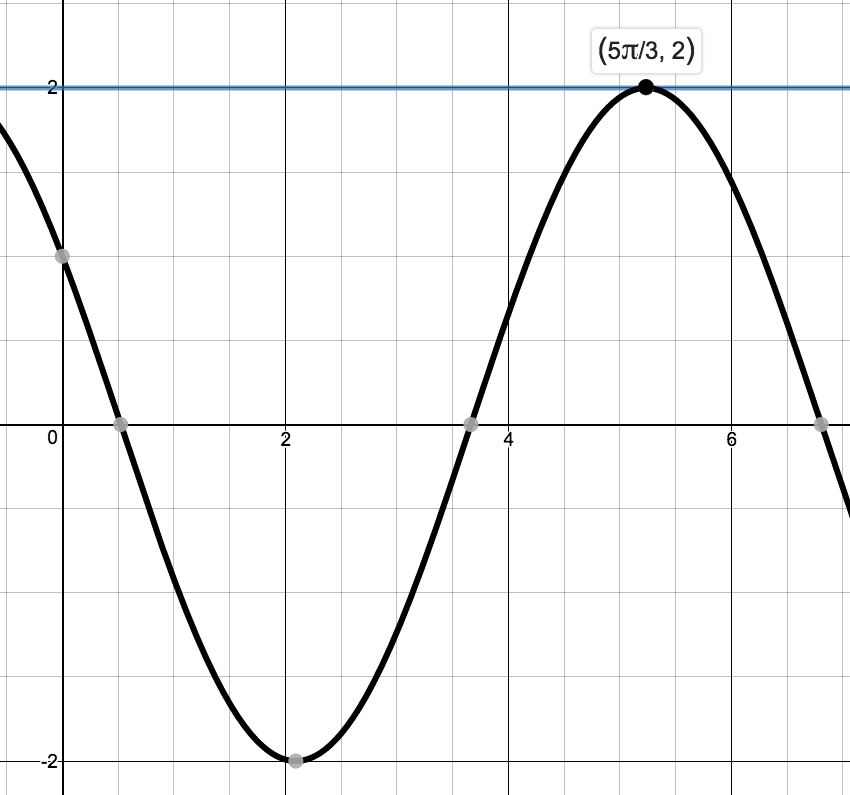
\includegraphics[height=2.25in]{./TrigonometricEquationsandInequalitiesGraphics/TrigEquIneq14.jpg} 

{\boldmath  $y = \cos(x) - \sqrt{3} \sin(x)$} and  $y = 2$

\end{center}

An alternative way to solve this problem is to \textit{introduce} squares in order to exchange sines and cosines using a Pythagorean Identity. 

\smallskip

 From  $\cos(x) - \sqrt{3} \sin(x) = 2$ we get $\sqrt{3} \sin(x) = \cos(x) - 2$ so that $\left(\sqrt{3} \sin(x)\right)^2 = \left(\cos(x) - 2\right)^2$.  Simplifying, we get: $3 \sin^{2}(x) = \cos^{2}(x) - 4 \cos(x) + 4$.
 
 \smallskip
 
 Substituting $\sin^{2}(x) = 1 - \cos^{2}(x)$, we get $3(1 - \cos^{2}(x)) = \cos^{2}(x) - 4\cos(x) + 4$ which results in the quadratic equation: $4 \cos^{2}(x) - 4 \cos(x) +1 = 0$.  
 
 \smallskip
 
 Letting $u = \cos(x)$, we get $4u^2 - 4u + 1 = 0$ or $(2u - 1)^2 = 0$.  We get $u = \cos(x) = \frac{1}{2}$.  Solving $\cos(x) = \frac{1}{2}$ gives $x = \frac{\pi}{3} + 2\pi k$ as well as $x = \frac{5\pi}{3} + 2\pi k$ for integers, $k$.  
 
 \smallskip
 
 Of these two families, only  solutions of the form $x = \frac{5\pi}{3} + 2\pi k$ checks in our original equation.\footnote{We've seen how squaring both sides can lead to extraneous solutions in Section \ref{AppRadEqus} and Chapter \ref{RootRadicalPowerFunctions}.  Here, squaring both sides admits an entire \textit{family} of extraneous solutions.}  We leave it the reader to verify this representation of solutions to $\cos(x) - \sqrt{3} \sin(x) = 2$ is equivalent to the one we found previously. \qed

\end{enumerate}

\end{example}
 
We repeat here the advice given when solving systems of nonlinear equations in section \ref{NonLinearEquations} --  when it comes to solving equations involving the circular functions, it helps to just try something.  

\smallskip

Next, we focus on solving inequalities involving the circular functions.  Since these functions are continuous on their domains, we may use the sign diagram technique we've used in the past to solve the inequalities.\footnote{See pages \pageref{firstsigndiagram}, \pageref{rationalsigndiagram},  \pageref{algebraicsigndiagram}, as well as Examples \ref{expineq} and \ref{logineq} for a review of this technique, as needed.}

\begin{example}  \label{TrigIneqEx1} Solve the following inequalities on $[0,2\pi)$.  Express your answers using interval notation and verify your answers graphically.

\begin{multicols}{3}

\begin{enumerate}

\item  $2\sin(t) \leq 1$

\item  $\sin(2x) > \cos(x)$

\item  $\tan(x) \geq 3$

\end{enumerate}

\end{multicols}

\newpage

{\bf Solution.}

\begin{enumerate}

\item  We begin solving $2\sin(t) \leq 1$ by collecting all of the terms on one side of the equation and zero on the other to get $2\sin(t) - 1 \leq 0$.  

\smallskip

Next, we let $f(t) = 2\sin(t) - 1$ and note that our original inequality is equivalent to solving $f(t) \leq 0$. We now look to see where, if ever, $f$ is undefined and where $f(t) = 0$.  

\smallskip

Since the domain of $f$ is all real numbers, we can immediately set  about finding the zeros of $f$.  Solving $f(t) = 0$, we have $2\sin(t) - 1=0$ or $\sin(t) = \frac{1}{2}$.  The solutions here are $t = \frac{\pi}{6} + 2\pi k$ and $t = \frac{5\pi}{6} + 2\pi k$ for integers $k$.  Since we are restricting our attention to $[0,2\pi)$, only $t = \frac{\pi}{6}$ and $t = \frac{5\pi}{6}$ are of concern.

\smallskip

 Next, we choose test values in $[0,2\pi)$ other than the zeros and determine if $f$ is positive or negative there.  For $t = 0$ we have $f(0) = -1$, for $t = \frac{\pi}{2}$ we get $f\left(\frac{\pi}{2}\right) = 1$ and for $t = \pi$ we get $f(\pi) = -1$.  
 
 \smallskip
 
 Since our original inequality is equivalent to $f(t) \leq 0$, we are looking for where the function is negative $(-)$ or $0$, and we get the intervals $\left[0, \frac{\pi}{6}\right] \cup \left[\frac{5\pi}{6}, 2\pi \right)$.  We can confirm our answer graphically by seeing where the graph of $y = 2\sin(t)$ crosses or is below the graph of $y = 1$. 

\begin{center}

\begin{mfpic}[10]{-6}{6}{-2}{2}
\polyline{(-6,0),(6,0)}
\xmarks{-6,-2,2,6}
\tiny
\tlpointsep{6pt}
\normalsize
\tlabel[cc](-6,-1){$0$}
\tlabel[cc](-4,1){$(-)$}
\tlabel[cc](-2,-1){$\frac{\pi}{6}$}
\tlabel[cc](-2,1){0}
\tlabel[cc](0,1){$(+)$}
\tlabel[cc](2,-1){$\frac{5\pi}{6}$}
\tlabel[cc](2,1){$0$}
\tlabel[cc](4,1){$(-)$}
\tlabel[cc](6,-1){$2\pi$}
\end{mfpic} 



 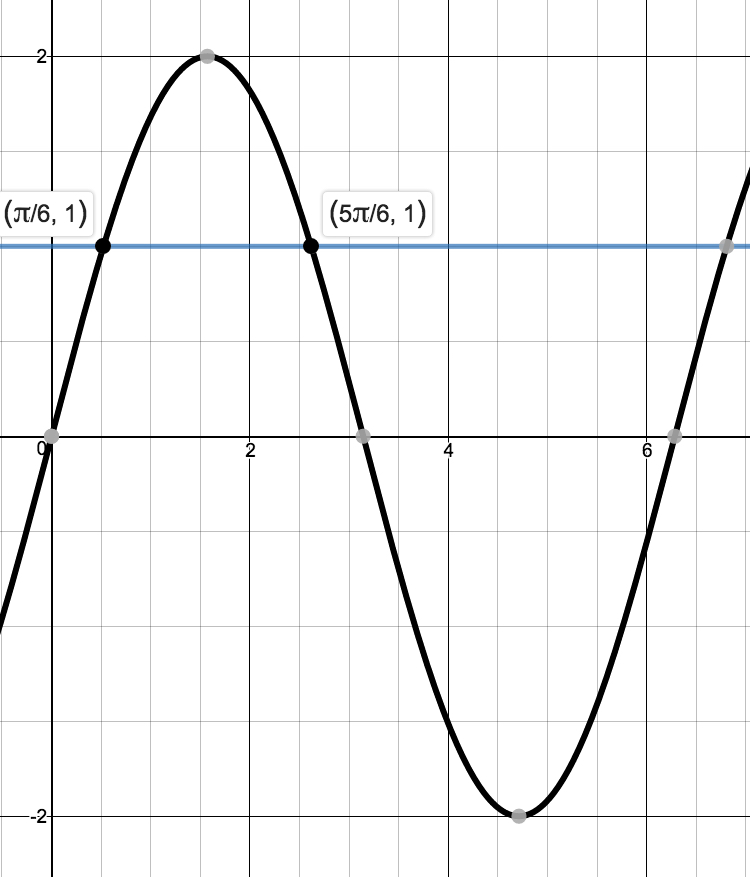
\includegraphics[height=2.5in]{./TrigonometricEquationsandInequalitiesGraphics/TrigEquIneq15.jpg}
 
 {\boldmath $y = 2\sin(t)$} and $y = 1$ 



\end{center}


\item  We first rewrite  $\sin(2x) > \cos(x)$   as $\sin(2x) - \cos(x) > 0$ and let $f(x) = \sin(2x) - \cos(x)$.  

\smallskip

Our original inequality is thus equivalent to $f(x) > 0$.  The domain of $f$ is all real numbers, so we can advance to finding the zeros of $f$. 

\smallskip

Setting $f(x) = 0$ yields $\sin(2x) - \cos(x) = 0$, which, by way of the double angle identity for sine, becomes $2\sin(x)\cos(x) - \cos(x) = 0$ or $\cos(x) (2\sin(x) - 1) = 0$.  

\smallskip

From $\cos(x) = 0$, we get $x = \frac{\pi}{2} + \pi k$ for integers $k$ of which only $x = \frac{\pi}{2}$ and $x = \frac{3\pi}{2}$ lie in $[0,2\pi)$.  

\smallskip

For $2\sin(x) - 1 = 0$, we get $\sin(x) = \frac{1}{2}$ which gives $x = \frac{\pi}{6} + 2\pi k$ or $x = \frac{5\pi}{6} + 2\pi k$ for integers $k$.  Of those, only $x = \frac{\pi}{6}$ and $x = \frac{5\pi}{6}$ lie in $[0,2\pi)$.  

\smallskip

Choosing test values, we get: for  $x =0$ we find $f(0) = -1$; when $x = \frac{\pi}{4}$ we get $f\left(\frac{\pi}{4}\right) =1 - \frac{\sqrt{2}}{2} = \frac{2 - \sqrt{2}}{2}$;  for $x = \frac{3\pi}{4}$ we get $f\left(\frac{3\pi}{4}\right) =-1 + \frac{\sqrt{2}}{2} =  \frac{\sqrt{2} - 2}{2}$;  when $x=\pi$ we have $f(\pi) = 1$, and lastly, for $x = \frac{7\pi}{4}$ we get $f\left(\frac{7\pi}{4}\right) = -1 - \frac{\sqrt{2}}{2} =  \frac{-2 - \sqrt{2}}{2}$.  

\smallskip

We see $f(x) > 0$ on $\left(\frac{\pi}{6}, \frac{\pi}{2}\right) \cup \left(\frac{5\pi}{6}, \frac{3\pi}{2}\right)$, so this is our answer.  Geometrically, we see the graph of $y = \sin(2x)$ is indeed above the graph of $y = \cos(x)$ on those intervals. 

\begin{center}


\begin{mfpic}[10]{-10}{10}{-2}{2}
\polyline{(-10,0),(10,0)}
\xmarks{-10,-6,-2,2,6,10}
\tiny
\tlpointsep{6pt}
\normalsize
\tlabel[cc](-10,-1){$0$}
\tlabel[cc](-8,1){$(-)$}
\tlabel[cc](-6,-1){$\frac{\pi}{6}$}
\tlabel[cc](-6,1){0}
\tlabel[cc](-4,1){$(+)$}
\tlabel[cc](-2,-1){$\frac{\pi}{2}$}
\tlabel[cc](-2,1){0}
\tlabel[cc](0,1){$(-)$}
\tlabel[cc](2,-1){$\frac{5\pi}{6}$}
\tlabel[cc](2,1){0}
\tlabel[cc](4,1){$(+)$}
\tlabel[cc](6,-1){$\frac{3\pi}{2}$}
\tlabel[cc](6,1){0}
\tlabel[cc](8,1){$(-)$}
\tlabel[cc](10,-1){$2\pi$}
\end{mfpic} 

 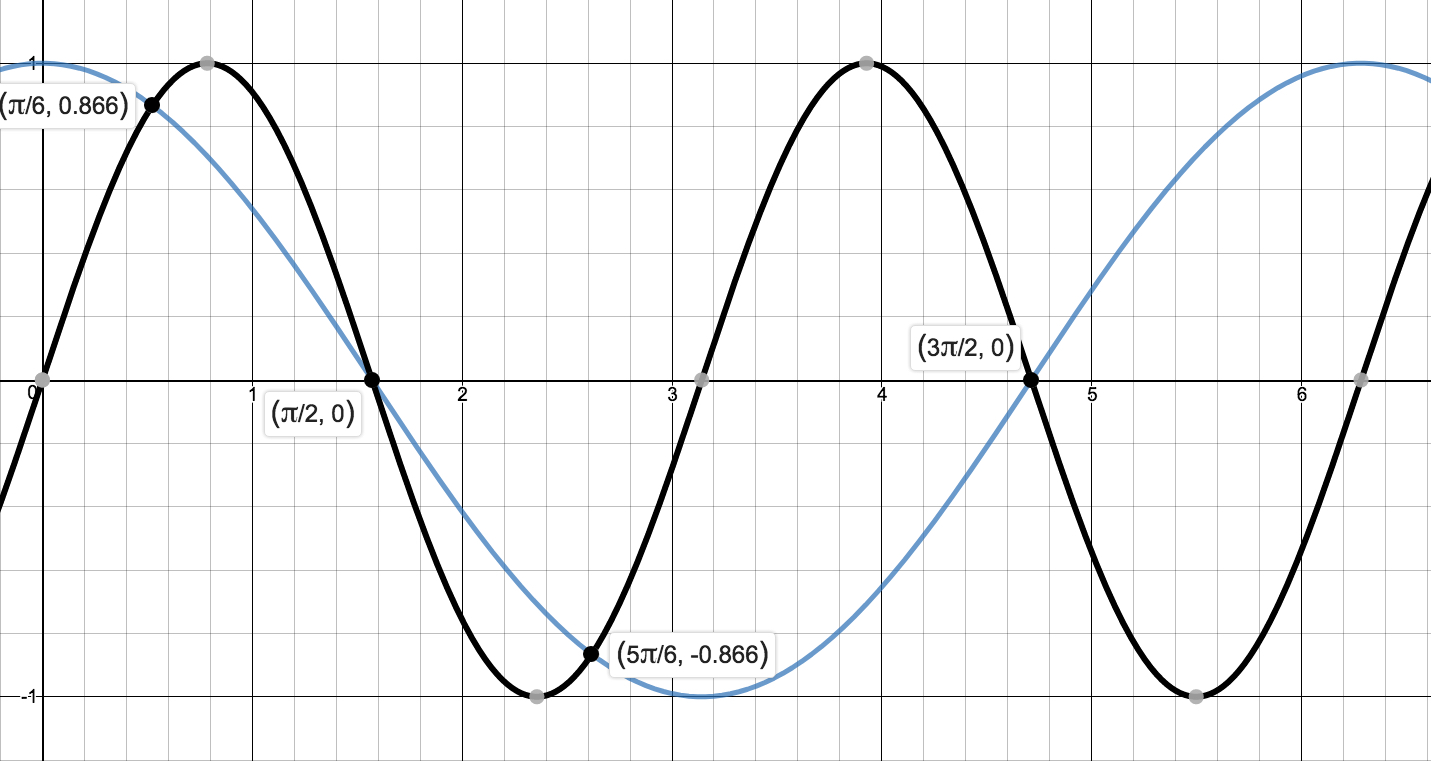
\includegraphics[height=2.5in]{./TrigonometricEquationsandInequalitiesGraphics/TrigEquIneq16.jpg}

 {\boldmath $y = \sin(2x)$} and  $y = \cos(x)$ 

\end{center}

\item  Proceeding as above, we rewrite  $\tan(x) \geq 3$ as $\tan(x) - 3 \geq 0$ and let $f(x) = \tan(x) - 3$.  

\smallskip

We note that on $[0,2\pi)$, $f$ is undefined at $x =\frac{\pi}{2}$ and $\frac{3\pi}{2}$, so those values will need the usual disclaimer on the sign diagram.\footnote{See page \pageref{rationalsigndiagram} for a discussion of the non-standard character known as the interrobang.}  

\smallskip

Moving along to zeros, solving $f(x) = \tan(x) - 3 = 0$ requires the arctangent function.  We find $x = \arctan(3) + \pi k$ for integers $k$ and of these, only $x = \arctan(3)$ and $x = \arctan(3) + \pi$ lie in $[0,2\pi)$.  Since $3 > 0$, we know $0 < \arctan(3) < \frac{\pi}{2}$ which allows us to position these zeros correctly on the sign diagram. 

\smallskip

To choose test values, we begin with $x=0$ and find $f(0) = -3$. Finding a convenient test value in the interval $\left(\arctan(3), \frac{\pi}{2}\right)$ is a bit more challenging.  Since the arctangent function is increasing and is bounded above by $\frac{\pi}{2}$,  the number $x = \arctan(117)$ is guaranteed\footnote{We could have chosen any value $\arctan(t)$ where $t > 3$.} to lie between  $\arctan(3)$ and $\frac{\pi}{2}$.  We see that $f(\arctan(117)) = \tan(\arctan(117)) - 3 = 114$.  

\smallskip

For our next test value, we take $x = \pi$ and find $f(\pi) = -3$, which brings us to finding a test value in the interval $\left(\arctan(3) + \pi, \frac{3\pi}{2} \right)$.

\smallskip

From $\arctan(3) < \arctan(117) < \frac{\pi}{2}$ we get $\arctan(3) + \pi < \arctan(117) + \pi < \frac{3\pi}{2}$ by adding $\pi$ through the inequality.  We find $f(\arctan(117)+\pi) = \tan(\arctan(117) + \pi) -3 = \tan(\arctan(117)) - 3 = 114$.  

\smallskip

For our last test value, we choose $x = \frac{7\pi}{4}$ and find $f\left(\frac{7\pi}{4}\right) = -4$.  

\smallskip

Since we want $f(x) \geq 0$, we see that our answer is $\left[ \arctan(3), \frac{\pi}{2}\right) \cup  \left[\arctan(3)+\pi, \frac{3\pi}{2}\right)$.  Using the graphs of $y = \tan(x)$ and $y = 3$, we see when the graph of the former is above (or meets) the graph of the latter. (Note, $\arctan(3) \approx 1.249$ and $\arctan(3) + \pi \approx 4.391$.)

\begin{center}

\begin{mfpic}[10]{-10}{10}{-2}{2}
\polyline{(-10,0),(10,0)}
\xmarks{-10,-6,-2,2,6,10}
\tiny
\tlpointsep{6pt}
\normalsize
\tlabel[cc](-10,-1){$0$}
\tlabel[cc](-8,1){$(-)$}
\tlabel[cc](-6,-1){\tiny $\arctan(3)$}
\tlabel[cc](-6,1){0}
\tlabel[cc](-4,1){$(+)$}
\tlabel[cc](-2,-1){$\frac{\pi}{2}$}
\tlabel[cc](-2,1){\textinterrobang}
\tlabel[cc](0,1){$(-)$}
\tlabel[cc](2,-1){\tiny $(\arctan(3)+\pi)$}
\tlabel[cc](2,1){0}
\tlabel[cc](4,1){$(+)$}
\tlabel[cc](6,-1){$\frac{3\pi}{2}$}
\tlabel[cc](6,1){\textinterrobang}
\tlabel[cc](8,1){$(-)$}
\tlabel[cc](10,-1){$2\pi$}
\end{mfpic} 

 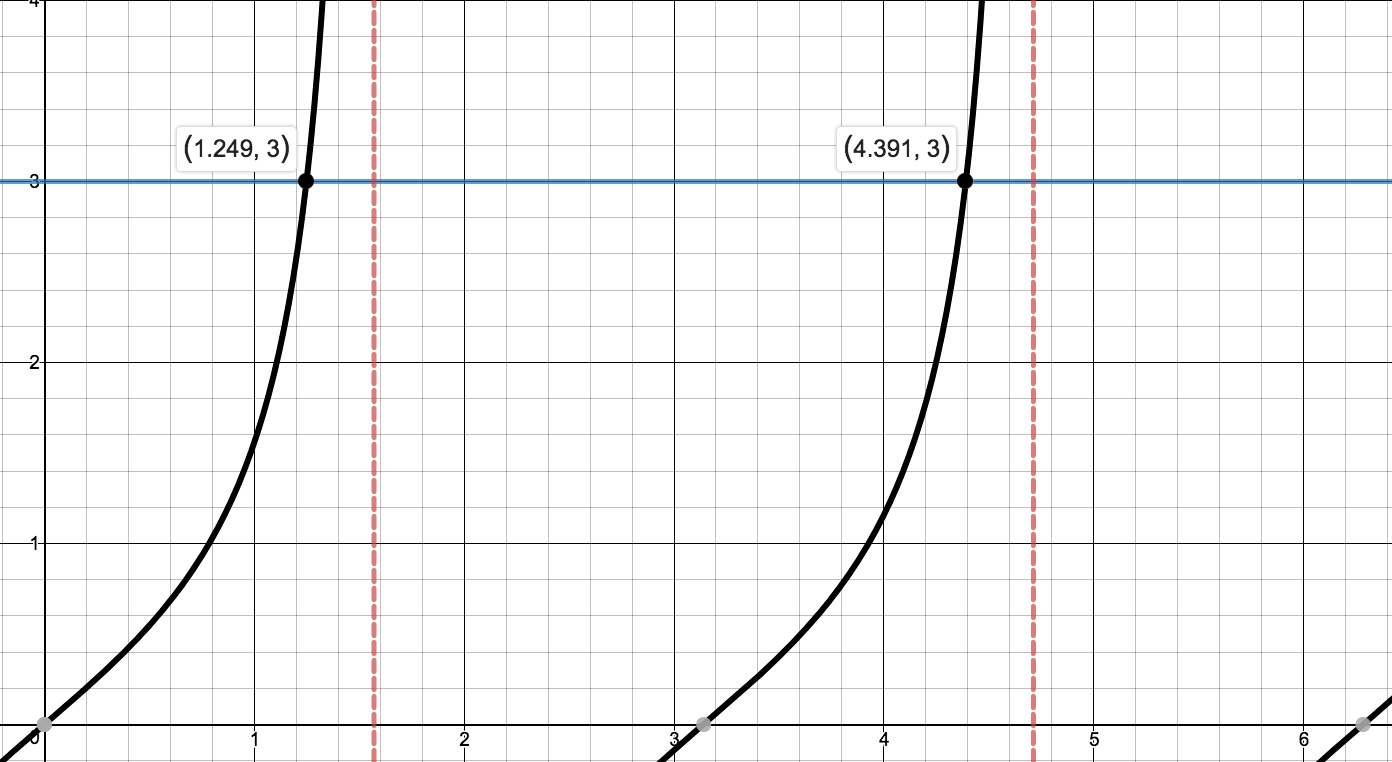
\includegraphics[height=2.5in]{./TrigonometricEquationsandInequalitiesGraphics/TrigEquIneq17.jpg} 
 
 {\boldmath $y = \tan(x)$} and $y =3$ 

\end{center}


\vspace{-.25in} \qed

\end{enumerate}


\end{example}


Our next example puts solving equations and inequalities to good use -- finding domains of functions.


\begin{example}  \label{TrigDomainEx1} Express the domain of the following functions using extended interval notation.\footnote{See Section \ref{extendedinterval} for details about this notation.}

\begin{multicols}{3}

\begin{enumerate}

\item  $f(x) = \csc\left(2x + \frac{\pi}{3}\right)$

\item  $f(t) = \dfrac{\sin(t)}{2\cos(t) - 1}$

\item  $f(x) = \sqrt{1 - \cot(x)}$

\end{enumerate}

\end{multicols}

\newpage

{\bf Solution.}

\begin{enumerate}

\item  To find the domain of $f(x) = \csc\left(2x + \frac{\pi}{3}\right)$, we rewrite $f$ in terms of sine as $f(x) = \frac{1}{\sin\left(2x + \frac{\pi}{3}\right)}$.  Since the sine function is defined everywhere, our only concern comes from zeros in the denominator.  

\smallskip

Solving $\sin\left(2x + \frac{\pi}{3}\right) = 0$, we get $x = -\frac{\pi}{6} + \frac{\pi}{2} k$ for integers $k$.  In set-builder notation, our domain is  $\left\{ x \, | \, x  \neq  -\frac{\pi}{6} + \frac{\pi}{2} k \, \text{for integers $k$} \right\}$.  To help visualize the domain,  we follow the old mantra `When in doubt, write it out!' We get $\left\{ x \, | \, x  \neq  -\frac{\pi}{6}, \frac{2\pi}{6}, -\frac{4\pi}{6}, \frac{5\pi}{6}, -\frac{7\pi}{6}, \frac{8\pi}{6}, \ldots \right\}$, where we have kept the denominators $6$ throughout to help see the pattern.  Graphing the situation on a number line, we have

\begin{center}

\begin{mfpic}[15]{-6}{6}{-1}{2}
\arrow \reverse \arrow \polyline{(-6,0), (6,0)}
\xmarks{-5,-3,-1,1,3,5}
\tlpointsep{5pt}
\axislabels {x}{{\small $-\frac{7\pi}{6} \hspace{7pt}$} -5,{\small $-\frac{4\pi}{6} \hspace{7pt}$} -3, {\small $-\frac{\pi}{6} \hspace{7pt}$} -1,{\small $\frac{2\pi}{6}$} 1,{\small $\frac{5\pi}{6}$} 3,  {\small $\frac{8\pi}{6}$} 5}

\penwd{1.5}
\arrow \reverse \arrow \polyline{(-5.75,1), (5.75,1)}

\penwd{0.75}

\gclear \circle{(-5,1),0.15}
\circle{(-5,1),0.15}

\gclear \circle{(-3,1),0.15}
\circle{(-3,1),0.15}

\gclear \circle{(-1,1),0.15}
\circle{(-1,1),0.15}

\gclear \circle{(5,1),0.15}
\circle{(5,1),0.15}

\gclear \circle{(3,1),0.15}
\circle{(3,1),0.15}

\gclear \circle{(1,1),0.15}
\circle{(1,1),0.15}

\end{mfpic}

\end{center}

Proceeding as in Section \ref{extendedinterval}, we let $x_{\mbox{\tiny $k$}}$ denote the $k$th number excluded from the domain and we have  $x_{\mbox{\tiny $k$}} = -\frac{\pi}{6} + \frac{\pi}{2} k = \frac{(3k-1)\pi}{6}$ for integers $k$.  The intervals which comprise the domain are of the form $\left(x_{\mbox{\tiny $k$}}, x_{\mbox{\tiny $k+1$}}  \right) = \left(\frac{(3k-1)\pi}{6}, \frac{(3k+2)\pi}{6} \right)$ as $k$ runs through the integers.  Using extended interval notation, we have that the domain is

\[ \bigcup_{k = -\infty}^{\infty}  \left(\dfrac{(3k-1)\pi}{6}, \dfrac{(3k+2)\pi}{6} \right)\]

We can check our answer by substituting in values of $k$ to see that it matches our diagram.


\item  Since the domains of $\sin(t)$ and $\cos(t)$ are all real numbers, the only concern when finding the domain of  $f(t) =  \frac{\sin(t)}{2\cos(t) - 1}$ is division by zero so we set the denominator equal to zero and solve. 

\smallskip

From $2\cos(t) - 1 = 0$ we get $\cos(t) = \frac{1}{2}$ so $t = \frac{\pi}{3} + 2\pi k$ or $t = \frac{5\pi}{3} + 2\pi k$ for integers $k$.  Using set-builder notation, the domain is $\left\{ t \, | \, t  \neq \frac{\pi}{3} + 2\pi k \, \text{and} \, t \neq \frac{5\pi}{3} + 2\pi k \, \text{for integers $k$} \right\}$. Writing this out, we find the domain is  $\left\{ t \, | \, t  \neq \pm \frac{\pi}{3}, \pm \frac{5\pi}{3}, \pm \frac{7\pi}{3}, \pm \frac{11\pi}{3}, \ldots \right\}$, so we have

\begin{center}

\begin{mfpic}[15]{-6}{6}{-1}{2}
\arrow \reverse \arrow \polyline{(-8,0), (8,0)}
\xmarks{-7,-5,-3,-1,1,3,5,7}
\tlpointsep{5pt}
\axislabels {x}{{\small $-\frac{11\pi}{3} \hspace{7pt}$} -7,{\small $-\frac{7\pi}{3} \hspace{7pt}$} -5,{\small $-\frac{5\pi}{3} \hspace{7pt}$} -3, {\small $-\frac{\pi}{3} \hspace{7pt}$} -1,{\small $\frac{\pi}{3}$} 1,{\small $\frac{5\pi}{3}$} 3,  {\small $\frac{7\pi}{3}$} 5,  {\small $\frac{11\pi}{3}$} 7}

\penwd{1.5}
\arrow \reverse \arrow \polyline{(-7.75,1), (7.75,1)}

\penwd{0.75}

\gclear \circle{(-7,1),0.15}
\circle{(-7,1),0.15}

\gclear \circle{(-5,1),0.15}
\circle{(-5,1),0.15}

\gclear \circle{(-3,1),0.15}
\circle{(-3,1),0.15}

\gclear \circle{(-1,1),0.15}
\circle{(-1,1),0.15}

\gclear \circle{(7,1),0.15}
\circle{(7,1),0.15}

\gclear \circle{(5,1),0.15}
\circle{(5,1),0.15}

\gclear \circle{(3,1),0.15}
\circle{(3,1),0.15}

\gclear \circle{(1,1),0.15}
\circle{(1,1),0.15}


\end{mfpic}

\end{center}

Unlike the previous example, we have \textit{two} different families of points to consider, and we present two ways of dealing with this kind of situation.  One way is to generalize what we did in the previous example and use the formulas we found in our domain work to describe the intervals. 

\smallskip

 To that end, we let  $a_{\mbox{\tiny $k$}} = \frac{\pi}{3} + 2\pi k = \frac{(6k+1)\pi}{3}$ and  $b_{\mbox{\tiny $k$}} = \frac{5\pi}{3} + 2\pi k = \frac{(6k+5) \pi}{3}$ for integers $k$.  The goal now is to write the domain in terms of the $a$'s an $b$'s.  We find $a_{\mbox{\tiny $0$}} =  \frac{\pi}{3}$, $a_{\mbox{\tiny $1$}} =  \frac{7\pi}{3}$,  $a_{\mbox{\tiny $-1$}} =  -\frac{5\pi}{3}$, $a_{\mbox{\tiny $2$}} =  \frac{13\pi}{3}$, $a_{\mbox{\tiny $-2$}} =  -\frac{11\pi}{3}$, $b_{\mbox{\tiny $0$}} =  \frac{5\pi}{3}$,  $b_{\mbox{\tiny $1$}} =  \frac{11\pi}{3}$, $b_{\mbox{\tiny $-1$}} =  -\frac{\pi}{3}$,  $b_{\mbox{\tiny $2$}} =  \frac{17\pi}{3}$  and $b_{\mbox{\tiny $-2$}} =  -\frac{7\pi}{3}$.  
 
 \smallskip
 
 Hence, in terms of the $a$'s and $b$'s, our domain is

\[\ldots  \left(a_{\mbox{\tiny $-2$}}, b_{\mbox{\tiny $-2$}}  \right) \cup \left(b_{\mbox{\tiny $-2$}}, a_{\mbox{\tiny $-1$}}  \right)\cup \left(a_{\mbox{\tiny $-1$}}, b_{\mbox{\tiny $-1$}}  \right)\cup \left(b_{\mbox{\tiny $-1$}}, a_{\mbox{\tiny $0$}}  \right)\cup \left(a_{\mbox{\tiny $0$}}, b_{\mbox{\tiny $0$}}  \right)\cup \left(b_{\mbox{\tiny $0$}}, a_{\mbox{\tiny $1$}}  \right)\cup \left(a_{\mbox{\tiny $1$}}, b_{\mbox{\tiny $1$}}  \right)\cup \dots \]

If we group these intervals in pairs, $ \left(a_{\mbox{\tiny $-2$}}, b_{\mbox{\tiny $-2$}}  \right) \cup \left(b_{\mbox{\tiny $-2$}}, a_{\mbox{\tiny $-1$}}  \right)$, $\left(a_{\mbox{\tiny $-1$}}, b_{\mbox{\tiny $-1$}}  \right)\cup \left(b_{\mbox{\tiny $-1$}}, a_{\mbox{\tiny $0$}}  \right)$, $\left(a_{\mbox{\tiny $0$}}, b_{\mbox{\tiny $0$}}  \right)\cup \left(b_{\mbox{\tiny $0$}}, a_{\mbox{\tiny $1$}}  \right)$ and so forth, we see a pattern emerge of the form  $\left(a_{\mbox{\tiny $k$}}, b_{\mbox{\tiny $k$}}  \right)\cup \left(b_{\mbox{\tiny $k$}}, a_{\mbox{\tiny $k+1$}}  \right)$ for integers $k$ so that our domain can be written as 

\[ \bigcup_{k = -\infty}^{\infty} \left(a_{\mbox{\tiny $k$}}, b_{\mbox{\tiny $k$}}  \right)\cup \left(b_{\mbox{\tiny $k$}}, a_{\mbox{\tiny $k+1$}}  \right) =  \bigcup_{k = -\infty}^{\infty} \left(\frac{(6k+1)\pi}{3}, \frac{(6k+5) \pi}{3}  \right)\cup \left(\frac{(6k+5) \pi}{3}, \frac{(6k+7)\pi}{3}  \right) \]

A second approach to the problem exploits the periodic nature of $f$.  Since $\cos(t)$ and $\sin(t)$ have period $2\pi$, it's not too difficult to show the function $f$ repeats itself every $2\pi$ units.\footnote{This doesn't necessarily mean the period of $f$ is $2\pi$.  The tangent function is comprised of sine and cosine, but its period is half theirs.  The reader is invited to investigate the period of $f$.}  This means if we can find a formula for the domain on an interval of length $2\pi$, we can express the entire domain by translating our answer left and right on the $t$-axis by adding integer multiples of $2\pi$.

\smallskip

 One such interval that arises naturally from our domain work is  $\left[\frac{\pi}{3}, \frac{7\pi}{3}\right]$. The portion of the domain here is  $\left(\frac{\pi}{3}, \frac{5\pi}{3}\right) \cup \left(\frac{5\pi}{3}, \frac{7\pi}{3}\right)$.  Adding integer multiples of $2\pi$, we obtain the family of intervals:    $\left(\frac{\pi}{3} + 2\pi k, \frac{5\pi}{3} + 2\pi k \right) \cup \left(\frac{5\pi}{3} + 2\pi k, \frac{7\pi}{3} + 2\pi k\right)$ for integers $k$.  We leave it to the reader to show that getting common denominators leads to our previous answer.


\item  To find the domain of $f(x) = \sqrt{1-\cot(x)}$, we first note that, due to the presence of the $\cot(x)$ term, $x \neq \pi k$ for integers $k$.  

\smallskip

Next, we recall that for the square root to be defined, we need $1 - \cot(x) \geq 0$.  Unlike the inequalities we solved in Example \ref{TrigIneqEx1}, we are not restricted here to a given interval.  Our strategy is to solve this inequality over $(0,\pi)$  (the same interval which generates a fundamental cycle of cotangent) and then add integer multiples of the period, in this case, $\pi$.  

\smallskip

We let $g(x) = 1 - \cot(x)$ and set about making a sign diagram for $g$ over the interval $(0,\pi)$ to find where $g(x) \geq 0$.  We note that $g$ is undefined for $x = \pi k$ for integers $k$, in particular, at the endpoints of our interval $x = 0$ and $x = \pi$. 

\smallskip

Next, we look for the zeros of $g$.  Solving $g(x) = 0$, we get $\cot(x) = 1$ or $x = \frac{\pi}{4} + \pi k$ for integers $k$ and only one of these, $x = \frac{\pi}{4}$, lies in $(0,\pi)$.   Choosing the test values $x = \frac{\pi}{6}$ and $x = \frac{\pi}{2}$, we get $g\left(\frac{\pi}{6}\right) = 1 - \sqrt{3}$, and $g\left(\frac{\pi}{2}\right) = 1$.   We construct the sign diagram for $g$ over the interval $(0, \pi)$ below:

\begin{center}
\begin{mfpic}[10]{-2}{6}{-2}{2}
\polyline{(-2,0),(6,0)}
\xmarks{-2,2,6}
\tiny
\tlpointsep{6pt}
\normalsize
\tlabel[cc](-2,-1){$0$}
\tlabel[cc](-2,1){\textinterrobang}
\tlabel[cc](0,1){$(-)$}
\tlabel[cc](2,-1){$\frac{\pi}{4}$}
\tlabel[cc](2,1){$0$}
\tlabel[cc](4,1){$(+)$}
\tlabel[cc](6,-1){$\pi$}
\tlabel[cc](6,1){\textinterrobang}
\end{mfpic} 
\end{center}

We find $g(x) \geq 0$ on $\left[\frac{\pi}{4}, \pi \right)$.  Adding multiples of the period we get our solution to consist of the intervals  $\left[\frac{\pi}{4} + \pi k, \pi + \pi k  \right) = \left[\frac{(4k+1)\pi}{4}, (k+1)\pi \right)$.  

\smallskip

Using extended interval notation, we have our final answer:
\[\bigcup_{k = -\infty}^{\infty} \left[\dfrac{(4k+1)\pi}{4}, (k+1)\pi \right)\]



\end{enumerate}
\qed
\end{example}

In our next example, we solve equations and inequalities involving the \textit{inverse} circular functions.

\begin{example}  Solve the following equations and inequalities analytically.  Check your answers using a graphing utility.

\begin{multicols}{2}
\begin{enumerate}

\item  $\arcsin(2x) = \frac{\pi}{3}$

\item  $4\arccos(t)-3\pi = 0 \vphantom{\frac{\pi}{3}}$

\setcounter{HW}{\value{enumi}}
\end{enumerate}
\end{multicols}

\begin{multicols}{2}
\begin{enumerate}
\setcounter{enumi}{\value{HW}}

\item  $3 \, \text{arcsec}(2x-1) + \pi = 2 \pi$

\item  $4\arctan^2(t)-3\pi \arctan(t)-\pi^2 = 0$

\setcounter{HW}{\value{enumi}}
\end{enumerate}
\end{multicols}

\begin{multicols}{2}
\begin{enumerate}
\setcounter{enumi}{\value{HW}}

\item  $\pi^2-4\arccos^{2}(x) < 0$

\item  $4 \, \text{arccot}(3t) > \pi$



\end{enumerate}
\end{multicols}

{\bf Solution.} 
\begin{enumerate}

\item  To solve $\arcsin(2x) = \frac{\pi}{3}$, we first note that $\frac{\pi}{3}$ is in the range of the arcsine function (so a solution exists!) Next, we exploit the inverse property of sine and arcsine from Theorem \ref{arccosinesinefunctionprops}

\[ \begin{array}{rclr}

\arcsin(2x) & = & \frac{\pi}{3} & \\
\sin\left(\arcsin(2x)\right) & = & \sin\left(\frac{\pi}{3}\right) & \\ [5pt]
2x & = & \frac{\sqrt{3}}{2} & \text{Since $\sin(\arcsin(u)) = u$} \\ [5pt]
x & = & \frac{\sqrt{3}}{4} & \\ \end{array} \]

Below we see the graphs of  $y = \arcsin(2x)$ and $y = \frac{\pi}{3}$, intersect at $x = \frac{\sqrt{3}}{4} \approx 0.4430$.

\begin{center}

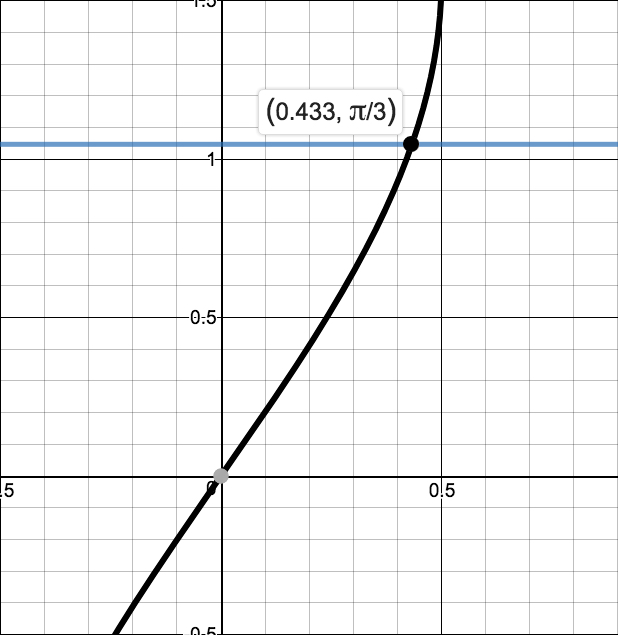
\includegraphics[height=2.5in]{./TrigonometricEquationsandInequalitiesGraphics/ARCSINEQN.jpg}

{\boldmath $y = \arcsin(2x)$} and  $y = \frac{\pi}{3}$

\end{center}

\item Our first step in solving $4\arccos(t)-3\pi = 0$ is to isolate the arccosine. We get $\arccos(t) = \frac{3\pi}{4}$.  Since $\frac{3\pi}{4}$ is in the range of arccosine, we may apply Theorem \ref{arccosinesinefunctionprops}

\[ \begin{array}{rclr}

\arccos(t) & = & \frac{3\pi}{4} & \\ [5pt]
\cos\left(\arccos(t)\right) & = & \cos\left(\frac{3\pi}{4}\right) & \\ [5pt]
t & = & -\frac{\sqrt{2}}{2} & \text{Since $\cos(\arccos(u)) = u$} \\ \end{array} \]


Below we see the graph of $y = 4\arccos(t) - 3\pi$ crosses $y = 0$ at $t=-\frac{\sqrt{2}}{2} \approx -0.7071$.

\begin{center}

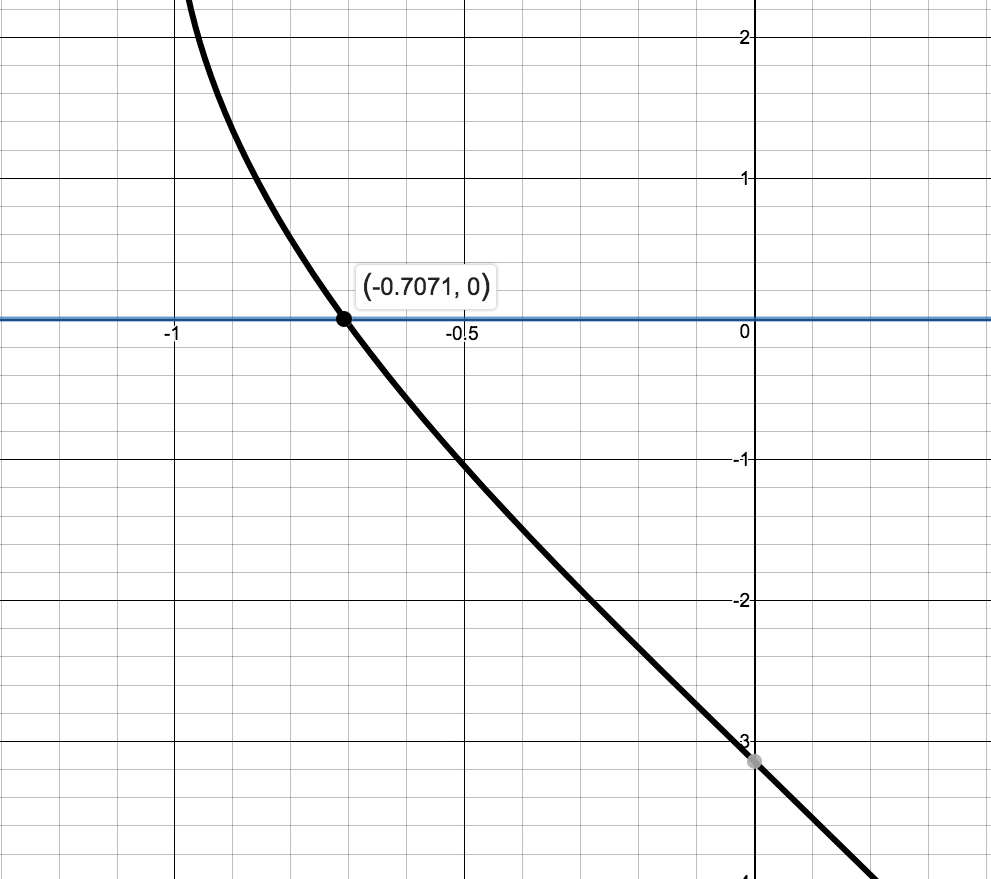
\includegraphics[height=2.5in]{./TrigonometricEquationsandInequalitiesGraphics/ARCCOSEQN.jpg}   

{\boldmath $y=4\arccos(t) - 3\pi$} and $y =0$ \\

\end{center}


\item From $3 \, \text{arcsec}(2x-1) + \pi = 2 \pi$, we get $\text{arcsec}(2x-1) = \frac{\pi}{3}$.  Regardless of how the range of arcsecant is chosen,  since $0 \leq \frac{\pi}{3} < \frac{\pi}{2}$, both Theorems \ref{arcsecantcosecantfunctionprops1}  \ref{arcsecantcosecantfunctionprops2}, apply:

\[ \begin{array}{rclr}

\text{arcsec}(2x-1)& = & \frac{\pi}{3} & \\ [5pt]
\sec(\text{arcsec}(2x-1)) & = & \sec\left(\frac{\pi}{3}\right) & \\ [5pt]
2x -1 & = & 2 & \text{Since $\sec(\text{arcsec}(u)) = u$} \\ [5pt]
    x & = & \frac{3}{2} \\ \end{array} \]

Below we see the graphs of $y=3 \, \text{arcsec}(2x-1) + \pi$ and  $y = 2\pi$ intersect at $x=\frac{3}{2} = 1.5$.

\begin{center}

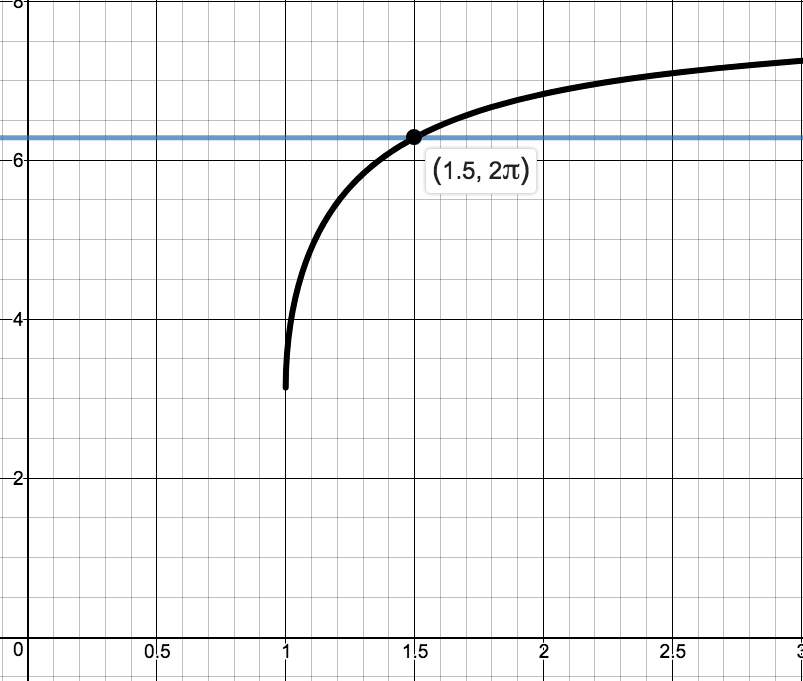
\includegraphics[height=2.5in]{./TrigonometricEquationsandInequalitiesGraphics/ARCSECEQN.jpg} 

{\boldmath $y = 3 \, \text{arcsec}(2x-1) + \pi$} and $y = 2\pi$  

\end{center}

\item  With the presence of both $\arctan^{2}(t)$ ( $= (\arctan(t))^2$) and $\arctan(t)$, we substitute $u = \arctan(t)$ to reveal a quadratic in disguise:  $4u^2 -3\pi u - \pi^2 = 0$.  

\smallskip

Factoring, (don't let the $\pi$ throw you!) we get $(4u+\pi)(u - \pi) = 0$, so $u = \arctan(t) = -\frac{\pi}{4}$ or $u = \arctan(t) = \pi$.  

\smallskip

Since $-\frac{\pi}{4}$ is in the range of arctangent, but $\pi$ is not, we only get solutions from the first equation.  Using Theorem \ref{arctangentcotangentfunctionprops}, we get

\[ \begin{array}{rclr}

\arctan(t) & = & -\frac{\pi}{4} & \\ [5pt]
\tan(\arctan(t)) & = & \tan\left(-\frac{\pi}{4}\right) & \\ [5pt]
t & = & -1 & \text{Since $\tan(\arctan(u)) = u$.} \\ \end{array}\]

We verify this result graphically below.

\begin{center}

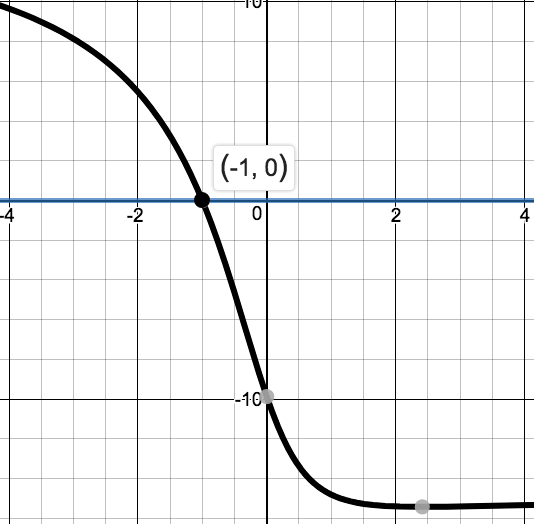
\includegraphics[width=2.2in]{./TrigonometricEquationsandInequalitiesGraphics/ARCTANEQN.jpg}  

{\boldmath  $y=4\arctan^2(t)-3\pi \arctan(t)-\pi^2$ } and $y=0$.\\

\end{center}

\item Since the inverse circular functions are continuous on their domains, we can solve inequalities featuring these functions using sign diagrams. 

\smallskip

Since all of the nonzero terms of  $\pi^2-4\arccos^{2}(x) < 0$ are on one side of the inequality, we let $f(x) = \pi^2-4\arccos^{2}(x)$ and note the domain of $f$ is limited by the $\arccos(x)$ to $[-1,1]$.  

\smallskip

Next, we find the zeros of $f$ by setting $f(x) = \pi^2-4\arccos^{2}(x) = 0$.  We get $\arccos(x) = \pm \frac{\pi}{2}$, and since the range of arccosine is $[0,\pi]$, we focus our attention on $\arccos(x) = \frac{\pi}{2}$.  

\smallskip

Using Theorem \ref{arccosinesinefunctionprops}, we get $x = \cos\left(\frac{\pi}{2}\right) = 0$ as our only zero which breaks our domain $[-1,1]$ into two test intervals: $[-1,0)$ and $(0,1]$.  

\smallskip

Choosing test values $x = \pm 1$, we get $f(-1) = -3\pi^2 < 0$ and $f(1) = \pi^2 > 0$.  Since we are looking for where $f(x) = \pi^2-4\arccos^{2}(x) < 0$, our answer is $[-1,0)$.  

\smallskip

Geometrically,  we find the graph of $y = \pi^2-4\arccos^{2}(x)$ is below $y = 0$ (the $x$-axis) on $[-1,0)$.


\begin{center}

\begin{mfpic}[10]{-5}{5}{-2}{2}
\polyline{(-5,0),(5,0)}
\xmarks{-5,0,5}
\tiny
\tlpointsep{6pt}
\normalsize
\tlabel[cc](-5,-1){$-1$}
\tlabel[cc](-2.5,1){$(-)$}
\tlabel[cc](0,1){$0$}
\tlabel[cc](0,-1){$0$}
\tlabel[cc](5,-1){$1$}
\tlabel[cc](2.5,1){$(+)$}
\end{mfpic} 


 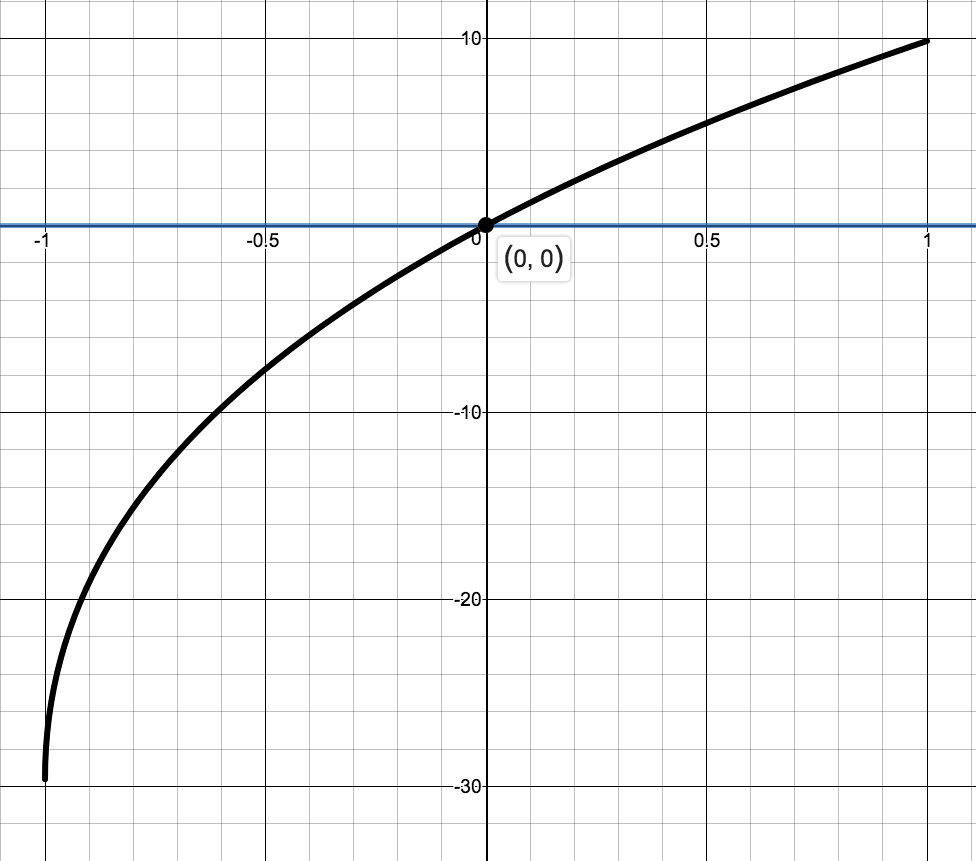
\includegraphics[height=2.5in]{./TrigonometricEquationsandInequalitiesGraphics/ARCCOSINEQ.jpg} \\

{\boldmath $y = \pi^2-4\arccos^{2}(x)$} and $y=0$  

\end{center}

\item   As in the previous problem, we will use a sign diagram to solve $4 \, \text{arccot}(3t) > \pi$.  Our first step is to rewrite the inequality as $4 \, \text{arccot}(3t) -  \pi > 0$. 

\smallskip

We let $f(t) = 4 \, \text{arccot}(3t) -  \pi$, and find the domain of $f$ is all real numbers, $(-\infty, \infty)$.  

\smallskip

To find the zeros of $f$, we set $f(t) = 4 \, \text{arccot}(3t) -  \pi = 0$ and solve.  We get $\text{arccot}(3t) = \frac{\pi}{4}$, and since $\frac{\pi}{4}$ is in the range of arccotangent, we may apply Theorem \ref{arctangentcotangentfunctionprops} and solve 

\[ \begin{array}{rclr}

\text{arccot}(3t) & = & \frac{\pi}{4} & \\ [5pt]
\cot(\text{arccot}(3t)) & = & \cot\left(\frac{\pi}{4}\right) & \\ [5pt]
3t & = & 1 & \text{Since $\cot(\text{arccot}(u)) = u$.} \\ [5pt]
t & = & \frac{1}{3} &  \\ \end{array}\]


Next, we make a sign diagram for $f$.  Since the domain of $f$ is all real numbers, and there is only one zero of $f$, $t = \frac{1}{3}$, we have two test intervals, $\left(-\infty, \frac{1}{3}\right)$ and  $\left(\frac{1}{3}, \infty \right)$.

\smallskip

 Ideally, we wish to find test values $t$ in these intervals so that $\text{arccot}(3t)$ corresponds to one of our oft-used `common' angles.  After a bit of computation,\footnote{Set $3t$ equal to the cotangents of the `common angles' and choose accordingly.} we choose $t=0$ for the interval  $\left(-\infty, \frac{1}{3}\right)$ and $t = \frac{\sqrt{3}}{3}$ for the interval $\left(\frac{1}{3}, \infty \right)$.
 
 \smallskip
 
 We find $f(0) = \pi > 0$ and $f\left(\frac{\sqrt{3}}{3}\right) = -\frac{\pi}{3} < 0$.  Since we are looking for where $f(t) > 0$, we get our answer $\left(-\infty, \frac{1}{3}\right)$.   Graphically, we see  the graph of $y = 4 \, \text{arccot}(3t)$  is above the horizontal line $y = \pi$ on $\left(-\infty, \frac{1}{3}\right)= \left(-\infty, 0.\overline{3} \right)$.



\begin{center}

\begin{mfpic}[10]{-5}{5}{-2}{2}
\arrow \reverse \arrow \polyline{(-5,0),(5,0)}
\xmarks{0}
\tiny
\tlpointsep{6pt}
\normalsize

\tlabel[cc](-2.5,1){$(+)$}
\tlabel[cc](0,1){$0$}
\tlabel[cc](0,-1){$\frac{1}{3}$}
\tlabel[cc](2.5,1){$(-)$}
\end{mfpic}

 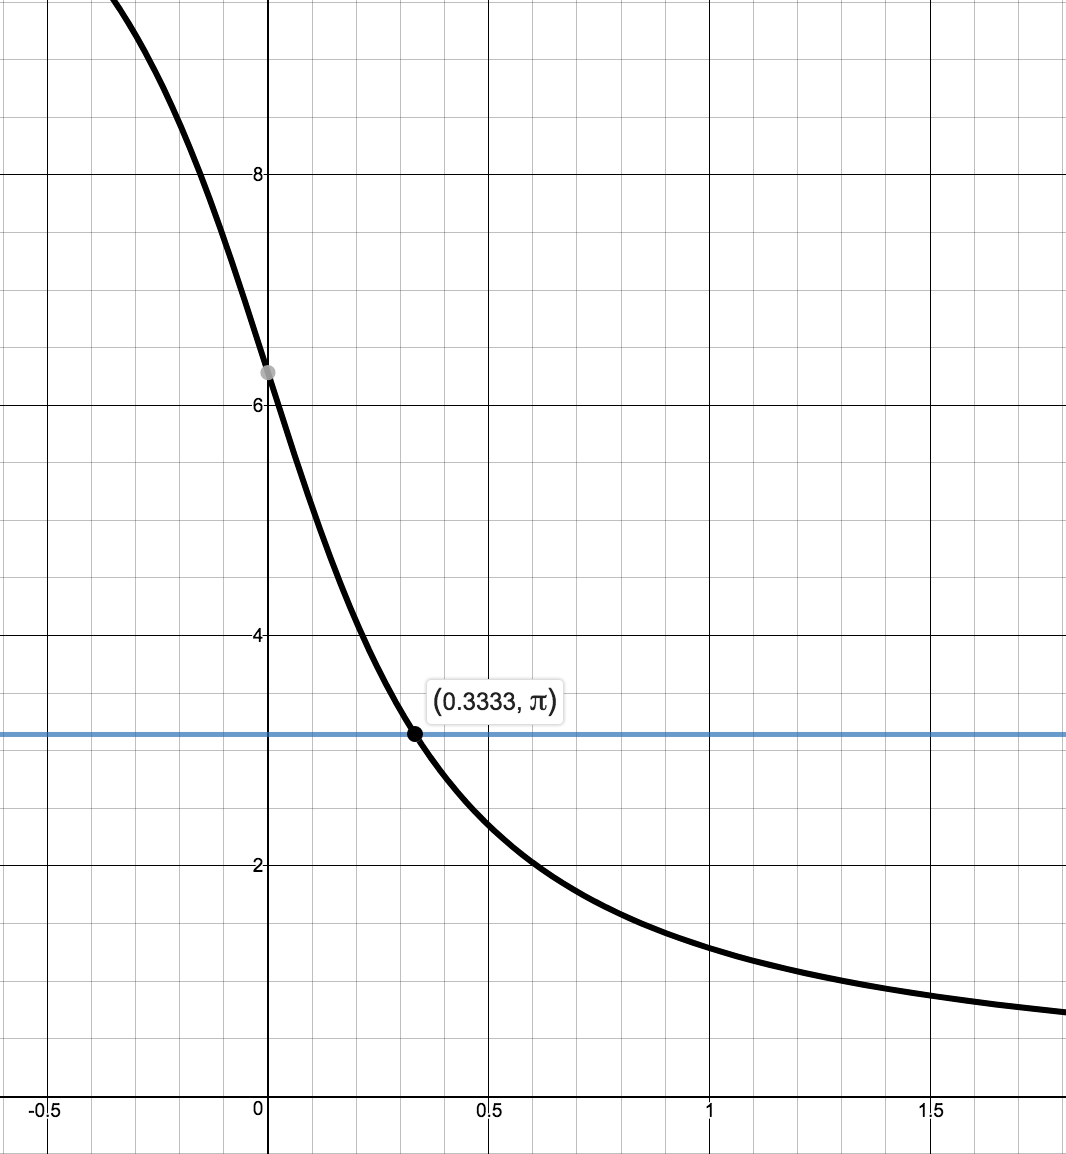
\includegraphics[height=2.5in]{./TrigonometricEquationsandInequalitiesGraphics/ARCCOTINEQ.jpg} 

 { \boldmath $y = 4 \, \text{arccot}(3t)$} and  $y=\pi$ 



\end{center}


\end{enumerate}

\vspace{-.25in} \qed

\end{example}

\newpage

\subsection{Harmonic Motion}
\label{harmomicmotion}

One of the major applications of the circular functions (sinusoids in particular!)  in Science and Engineering is the study of \index{harmonic motion} \textbf{harmonic motion},  We close this chapter with a brief foray into this topic since it pulls together many important concepts from both Chapters \ref{FoundationsofTrigonometry} and \ref{AnalyticalTrigonometry}.  The equations for harmonic motion can be used to describe a wide range of phenomena, from the motion of an object on a spring, to the response of an electronic circuit.  In this subsection, we restrict our attention to modeling a simple spring system.  Before we jump into the Mathematics, there are some Physics terms and concepts we need to discuss.  

\smallskip

In Physics, `mass' is defined as a measure of an object's resistance to straight-line motion whereas `weight' is the amount of force (pull) gravity exerts on an object.  An object's mass cannot change,\footnote{Well, assuming the object isn't subjected to relativistic speeds \dots} while its weight could change.  An object which weighs 6 pounds on the surface of the Earth would weigh 1 pound on the surface of the Moon, but its mass is the same in both places. In the English system of units, `pounds' (lbs.) is a measure of force (weight), and the corresponding unit of mass is the `slug'. In the SI system, the unit of force is `Newtons' (N) and the associated unit of mass is the `kilogram' (kg). 

\smallskip

We convert between mass and weight using the formula\footnote{This is a consequence of Newton's Second Law of Motion $F = ma$ where $F$ is force, $m$ is mass and $a$ is acceleration.  In our present setting, the force involved is weight which is caused by the acceleration due to gravity.} $w = mg$.   Here, $w$ is the weight of the object, $m$ is the mass and $g$ is the acceleration due to gravity.  In the English system, $g = 32 \frac{\text{feet}}{\text{second}^2}$, and in the SI system, $g = 9.8\frac{\text{meters}}{\text{second}^2}$. Hence, on Earth a \textit{mass} of 1 slug \textit{weighs} 32 lbs. and a \textit{mass} of 1 kg \textit{weighs} 9.8 N.\footnote{Note that $1$ pound $ = 1 \, \frac{\text{slug foot}}{\text{second}^2}$ and $1$ Newton $ = 1 \, \frac{\text{kg meter}}{\text{second}^2}$.}    Suppose we attach an object with mass $m$ to a spring as depicted below. 

\begin{center}

\begin{tabular}[t]{ccc}

\begin{mfpic}[15]{-3}{3}{-2}{5}
\dashed \polyline{(-3,0.5), (3,0.5)}
\hatchcolor[gray]{.7}
\lhatch \rect{(-3,4), (3,5)}
\fillcolor[gray]{.7} 
\gfill \rect{(-0.5,0), (0.5,1)}
\polyline{(0,4), (0,3.5), (0.25,3.25), (-0.25, 3), (0.25,2.75), (-0.25,2.5), (0.25,2.25), (-0.25,2), (0.25,1.75), (-0.25,1.5), (0, 1.25), (0,1)}
\penwd{1.025}
\rect{(-3,4), (3,5)}
\rect{(-0.5,0), (0.5,1)}
\drawcolor{white} \polyline{(-3,-2), (-3,2)}
\end{mfpic} 

&

\hspace{0.5in}
\begin{mfpic}[15]{-3}{3}{-2}{5}
\dashed \polyline{(-3,0.5), (3,0.5)}
\hatchcolor[gray]{.7}
\lhatch \rect{(-3,4), (3,5)}
\fillcolor[gray]{.7} 
\gfill \rect{(-0.5,0.95), (0.5,1.95)}
\polyline{(0,4), (0,3.5), (0.25,3.4), (-0.25, 3.25), (0.25,3.1), (-0.25,2.95), (0.25,2.8), (-0.25,2.65), (0.25,2.5), (-0.25,2.35), (0, 2.2), (0,1.95)}
\penwd{1.025}
\rect{(-3,4), (3,5)}
\rect{(-0.5,0.95), (0.5,1.95)}
\drawcolor{white} \polyline{(-3,-2), (-3,2)}
\end{mfpic} 

&

\hspace{0.5in}
\begin{mfpic}[15]{-3}{3}{-2}{5}
\dashed \polyline{(-3,0.5), (3,0.5)}
\hatchcolor[gray]{.7}
\lhatch \rect{(-3,4), (3,5)}
\fillcolor[gray]{.7} 
\gfill \rect{(-0.5,-1.35), (0.5,-0.35)}
\polyline{(0,4), (0,3.5), (0.25,3.1), (-0.25, 2.7), (0.25,2.3), (-0.25, 1.9), (0.25,1.5), (-0.25,1.1), (0.25,0.7), (-0.25,0.3), (0, -0.1), (0,-0.35)}
\penwd{1.025}
\rect{(-3,4), (3,5)}
\rect{(-0.5,-1.35), (0.5,-0.35)}
\drawcolor{white} \polyline{(-3,-2), (-3,2)}
\end{mfpic} \\
 
$x(t) = 0$ at the &
\hspace{0.5in}
$x(t) < 0$ above the&
\hspace{0.5in}
$x(t) > 0$ below the \\

equilibrium position & 
\hspace{0.5in}
equilibrium position & 
\hspace{0.5in}
equilibrium position \\

\end{tabular}

\end{center}

The weight of the object will stretch the spring.   The system is said to be in `equilibrium' when the weight of the object is perfectly balanced with the restorative force of the spring.  How far the spring stretches to reach equilibrium depends on the spring's `spring constant'. Usually denoted by the letter $k$, the spring constant relates the force $F$ applied to the spring to the amount $d$ the spring stretches in accordance with \href{http://en.wikipedia.org/wiki/Hooke's_law}{\underline{Hooke's Law}}\footnote{Look familiar?  We saw Hooke's Law in Section \ref{AppVariation}.} $F = kd$.  

\smallskip

If the object is released above or below the equilibrium position, or if the object is released with an upward or downward velocity, the object will bounce up and down on the end of the spring until some external force stops it.  If we let $x(t)$ denote the object's displacement from the equilibrium position at time $t$, then $x(t) = 0$ means the object is at the equilibrium position, $x(t) < 0$ means the object is \textit{above} the equilibrium position, and $x(t) > 0$ means the object is \textit{below} the equilibrium position.  The function $x(t)$ is called the `equation of motion' of the object.\footnote{To keep units compatible, if we are using the English system, we use feet (ft.) to measure displacement.  If we are in the SI system, we measure displacement in meters (m). Time is always measured in seconds (s).}

\smallskip


If we ignore all other influences on the system except gravity and the spring force, then Physics tells us that gravity and the spring force will battle each other forever and the object will oscillate indefinitely.  In this case, we describe the motion as `free' (meaning there is no external force causing the motion) and `undamped' (meaning we ignore friction caused by surrounding medium, which in our case is air).  

\smallskip

The following theorem, which comes from Differential Equations, gives $x(t)$ as a function of the mass $m$ of the object, the spring constant $k$, the initial displacement $x_{\text{\tiny $0$}}$ of the object and initial velocity $v_{\text{\tiny $0$}}$ of the object.  

\smallskip

As with $x(t)$, $x_{\text{\tiny $0$}} = 0$ means the object is released from the equilibrium position, $x_{\text{\tiny $0$}} < 0$ means the object is released \textit{above} the equilibrium position and $x_{\text{\tiny $0$}}>0$ means the object is released \textit{below} the equilibrium position.  As far as the initial velocity $v_{\text{\tiny $0$}}$ is concerned, $v_{\text{\tiny $0$}} =0 $ means the object is released `from rest,' $v_{\text{\tiny $0$}}<0$ means the object is heading \textit{upwards} and $v_{\text{\tiny $0$}}>0$ means the object is heading \textit{downwards}.\footnote{The sign conventions here are carried over from Physics.  If not for the spring, the object would fall towards the ground, which is the `natural' or `positive' direction.  Since the spring force acts in direct opposition to gravity,  any movement upwards is considered `negative'.}

\medskip

%% \colorbox{ResultColor}{\bbm
\begin{theorem} \label{freeundampedmotion} \textbf{Equation for Free Undamped Harmonic Motion:}  Suppose an object of  mass $m$ is suspended from a spring with spring constant $k$.  If the initial displacement from the equilibrium position is $x_{\text{\tiny $0$}}$ and the initial velocity of the object is $v_{\text{\tiny $0$}}$, then the displacement $x$ from the equilibrium position at time $t$ is given by  $x(t) = A \sin(\omega t + \phi)$ where

\begin{itemize}

\item  $\omega = \sqrt{\dfrac{k}{m}}$ and $A = \sqrt{x_{\text{\tiny $0$}}^2 + \left( \dfrac{v_{\text{\tiny $0$}}}{\omega}\right)^2}$

\item $A\sin(\phi) = x_{\text{\tiny $0$}}$ and $A\omega\cos(\phi) = v_{\text{\tiny $0$}}$.

\end{itemize} 

\end{theorem}

\smallskip

%% \ebm}

\medskip

It is a great exercise in `dimensional analysis' to verify that the formulas given in Theorem \ref{freeundampedmotion} work out so that $\omega$ has units $\frac{1}{s}$ and  $A$ has units ft. or m, depending on which system we choose.

\begin{example} \label{freeudampedex}  Suppose an object weighing  64 pounds stretches a spring 8 feet.  

\begin{enumerate}

\item  If the object is attached to the spring and released 3 feet below the equilibrium position from rest, find the equation of motion of the object, $x(t)$.  When does the object first pass through the equilibrium position?  Is the object heading upwards or downwards at this instant? 

\item  If the object is attached to the spring and released 3 feet below the equilibrium position with an upward velocity of $8$ feet  per second, find the equation of motion of the object, $x(t)$.  What is the longest distance the object travels \textit{above} the equilibrium position?  When does this first happen? Confirm your result using a graphing utility.

\end{enumerate}

{\bf Solution.} In order to use the formulas in Theorem \ref{freeundampedmotion}, we first need to determine the spring constant $k$ and the mass of the object $m$.  

\smallskip

To find $k$, we use Hooke's Law $F = kd$.  We know the object weighs $64$ lbs. and stretches the spring $8$ ft.. Using $F = 64$ and $d = 8$,  we get  $64  = k \cdot 8 $, or  $k = 8 \frac{\text{lbs.}}{\text{ft.}}$.  

\smallskip

To find $m$, we use $w = mg$ with $w = 64$ lbs. and $g =32 \frac{\text{ft.}}{s^2}$.  We get $m = 2$ slugs.  We can now proceed to apply Theorem \ref{freeundampedmotion}.

\begin{enumerate}

\item  With $k = 8$ and $m = 2$, we get $\omega = \sqrt{\frac{k}{m}} = \sqrt{\frac{8}{2}} = 2$.  Since the object is released 3 feet \textit{below} the equilibrium position `from rest,'    $x_{\text{\tiny $0$}} = 3$ and  $v_{\text{\tiny $0$}} = 0$.  Therefore, $A = \sqrt{x_{\text{\tiny $0$}}^2 + \left( \frac{v_{\text{\tiny $0$}}}{\omega}\right)^2} = \sqrt{3^2 + 0^2} = 3$.  

\smallskip

 To determine the phase $\phi$, we have $A\sin(\phi) = x_{\text{\tiny $0$}}$, which in this case gives $3 \sin(\phi) = 3$ so $\sin(\phi) = 1$.  Only $\phi = \frac{\pi}{2}$ and angles coterminal to it satisfy this condition, so we pick\footnote{For confirmation, we note that $A\omega\cos(\phi) = v_{\text{\tiny $0$}}$, which in this case reduces to $6\cos(\phi) = 0$.} the phase to be $\phi = \frac{\pi}{2}$.  Hence, the equation of motion is $x(t) = 3\sin\left(2t + \frac{\pi}{2}\right)$.  

\smallskip

To find when the object passes through the equilibrium position we solve $x(t)= 3\sin\left(2t + \frac{\pi}{2}\right) = 0$. Going through the usual analysis we find $t = -\frac{\pi}{4} + \frac{\pi}{2} k$ for integers $k$. Since we are interested in the \textit{first} time the object passes through the equilibrium position, we look for the smallest positive $t$ value which in this case is $t = \frac{\pi}{4} \approx 0.78$ seconds after the  start of the motion.  

\smallskip

Common sense suggests that if we release the object \textit{below} the equilibrium position, the object should be traveling \textit{upwards} when it first passes through it.   To check this answer, we graph one cycle of  $x(t)$.  Since our applied domain in this situation is $t \geq 0$, and the period of $x(t)$ is $T = \frac{2\pi}{\omega} = \frac{2\pi}{2} = \pi$, we graph $x(t)$ over the interval $[0,\pi]$.  Remembering that $x(t) > 0$ means the object is below the equilibrium position and $x(t) < 0$ means the object is above the equilibrium position, the fact our graph is crossing through the $t$-axis from positive $x$ to negative $x$ at $t = \frac{\pi}{4}$ confirms our answer.


\begin{center}

\begin{mfpic}[30][15]{-0.5}{4}{-3.25}{3.5}

\axes
\point[4pt]{(0,3), (0.78,0), (1.57,-3), (2.36,0), (3.14,3)}
\tlabel[cc](4,-0.5){\scriptsize $t$}
\tlabel[cc](0.5,3.5){\scriptsize $x$}
\xmarks{0.78, 1.57, 2.36, 3.14}
\ymarks{-3,-2,-1,1,2,3}
\tlabelsep{5pt}
\scriptsize
\axislabels{x}{{$\frac{\pi}{4}\hspace{7pt}$} 0.78, {$\frac{\pi}{2}$} 1.57,{$\frac{3\pi}{4}$} 2.36, {$\pi$} 3.14}
\axislabels{y}{{$-3$} -3, {$-2$} -2,{$-1$} -1, {$1$} 1,{$2$} 2,{$3$} 3}
\normalsize
\penwd{1.25pt}
\arrow \function{0, 0.65, 0.1}{3*sin(2*x+1.57)}
\arrow \function{0.65, 1, 0.1}{3*sin(2*x+1.57)}
\function{1, 3.14, 0.1}{3*sin(2*x+1.57)}
\end{mfpic}

$x(t)= 3\sin\left(2t + \frac{\pi}{2}\right)$

\end{center}

\item  The only difference between this problem and the previous problem is that we now release the object with an upward velocity of $8 \, \frac{\text{ft}}{s}$.  We still have $\omega = 2$ and $x_{\text{\tiny $0$}} = 3$, but now we have $v_{\text{\tiny $0$}} = -8$, the negative indicating the velocity is directed upwards. 

\smallskip

Here, we get $A = \sqrt{x_{\text{\tiny $0$}}^2 + \left( \frac{v_{\text{\tiny $0$}}}{\omega}\right)^2} = \sqrt{3^2 + (-4)^2} = 5$.  From $A\sin(\phi) = x_{\text{\tiny $0$}}$, we get $5\sin(\phi) = 3$ which gives $\sin(\phi) = \frac{3}{5}$.  From  $A\omega\cos(\phi) = v_{\text{\tiny $0$}}$, we get $10\cos(\phi) = -8$, or $\cos(\phi) = -\frac{4}{5}$.  

\smallskip

Hence,  $\phi$ is a Quadrant II angle which we can describe in terms of either arcsine or arccosine.  Since the range of arccosine covers Quadrant II, we choose to express $\phi$ in terms of the arccosine:  $\phi = \arccos\left( -\frac{4}{5} \right)$.  Hence, $x(t)= 5 \sin\left(2t + \arccos\left(-\frac{4}{5}\right) \right)$.  

\smallskip

Since the amplitude of $x(t)$ is $5$, the object will travel at most $5$ feet above the equilibrium position.  To find when this happens, we solve the equation $x(t)= 5 \sin\left(2t +\arccos\left( -\frac{4}{5} \right) \right)= -5$, the negative once again signifying that the object is \textit{above} the equilibrium position.  

\smallskip

Going through the usual machinations, we get $t = -\frac{1}{2} \arccos\left( -\frac{4}{5} \right)-\frac{\pi}{4}  + \pi k$ for integers $k$. The smallest (positive) of these values occurs when $k=1$, that is, $t =-\frac{1}{2} \arccos\left( -\frac{4}{5} \right)+ \frac{3\pi}{4}  \approx 1.107$ seconds after the start of the motion. 

\smallskip

Graphing $x(t) = 5 \sin\left(2t +  \arccos\left( -\frac{4}{5} \right) \right)$, we find the coordinates of the first relative minimum of to be approximately $(1.107,-5)$ .



\begin{center}


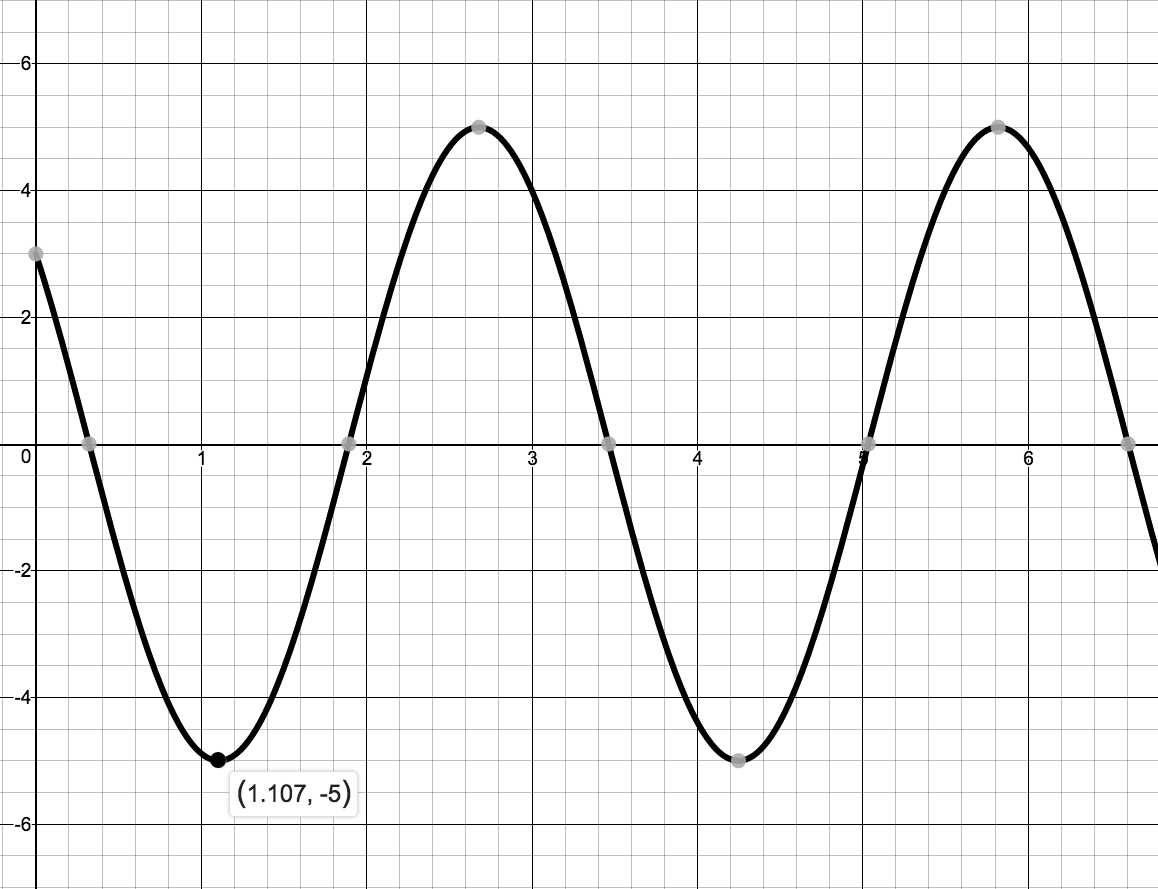
\includegraphics[height=2.5in]{./TrigonometricEquationsandInequalitiesGraphics/Sinusoid05.jpg} 

 $x(t) = 5 \sin\left(2t +  \arccos\left( -\frac{4}{5} \right) \right)$



\end{center}

\qed

\end{enumerate}
\end{example}

Though beyond the scope of this course, it is possible  to model the effects of friction and other external forces acting on the system.\footnote{Take a good Differential Equations class to see this!}  

\smallskip

While we may not have the Physics and Calculus background to \textit{derive} equations of motion for these scenarios, we can certainly analyze them.  We examine three cases in the following example.

\newpage

\begin{example} \label{underdampedresonance}  $~$  

\begin{enumerate}

\item  \label{underdampedproblem} Write $x(t) = 5e^{-t/5} \cos(t) + 5e^{-t/5} \sqrt{3} \sin(t)$ in the form $x(t) = A(t) \sin(\omega t + \phi)$.  Graph $x(t)$ using a graphing utility.

\item  Write $x(t) = (t+3)\sqrt{2} \cos(2t) + (t+3) \sqrt{2} \sin(2t)$ in the form $x(t) = A(t) \sin(\omega t + \phi)$.  Graph $x(t)$  using a graphing utility.

\item  Find the period of $x(t) = 5\sin(6t) - 5\sin\left(8t\right)$.  Graph $x(t)$ using a graphing utility.

\end{enumerate}

{\bf Solution.}

\begin{enumerate}

\item  We start rewriting  $x(t) = 5e^{-t/5} \cos(t) + 5e^{-t/5} \sqrt{3} \sin(t)$ by factoring out   $5e^{-t/5}$ from both terms to get  $x(t) = 5e^{-t/5} \left( \cos(t) + \sqrt{3} \sin(t)\right)$. We convert what's left in parentheses to the required form using the technique introduced in Example  \ref{expandedsinusoid} from Section \ref{MoreTrigonometricIdentities}.  We find $\left( \cos(t) + \sqrt{3} \sin(t)\right) = 2\sin\left(t+\frac{\pi}{3}\right)$ so that $x(t) = 10e^{-t/5} \sin\left(t + \frac{\pi}{3}\right)$.    


\smallskip

Graphing $x(t)$ reveals some interesting behavior.  The sinusoidal nature continues indefinitely, but it is being attenuated.  In the sinusoid $A \sin(\omega t + \phi)$, the coefficient $A$ of the sine function is the amplitude.  In the case of $x(t) = 10e^{-t/5} \sin\left(t + \frac{\pi}{3}\right)$, we can think of the \textit{function} $A(t) = 10e^{-t/5}$ as the amplitude.\footnote{This is the same sort of phenomenon we saw on page \pageref{beats} in Section \ref{expandedsinusoid}.}  Since $\ds{\lim_{t \rightarrow \infty} 10e^{-t/5} = 0}$, we can use the Squeeze Theorem, Theorem \ref{squeezeth} that $\ds{\lim_{t \rightarrow \infty} x(t) = 0}$.  (See Exercise \ref{squeezefordampedmotionexercise}).

Indeed, if we graph $x = \pm 10e^{-t/5}$ along with $x(t) = 10e^{-t/5} \sin\left(t + \frac{\pi}{3}\right)$, we see this attenuation taking place with the exponentials acting as a `wave envelope.'  

\begin{center}

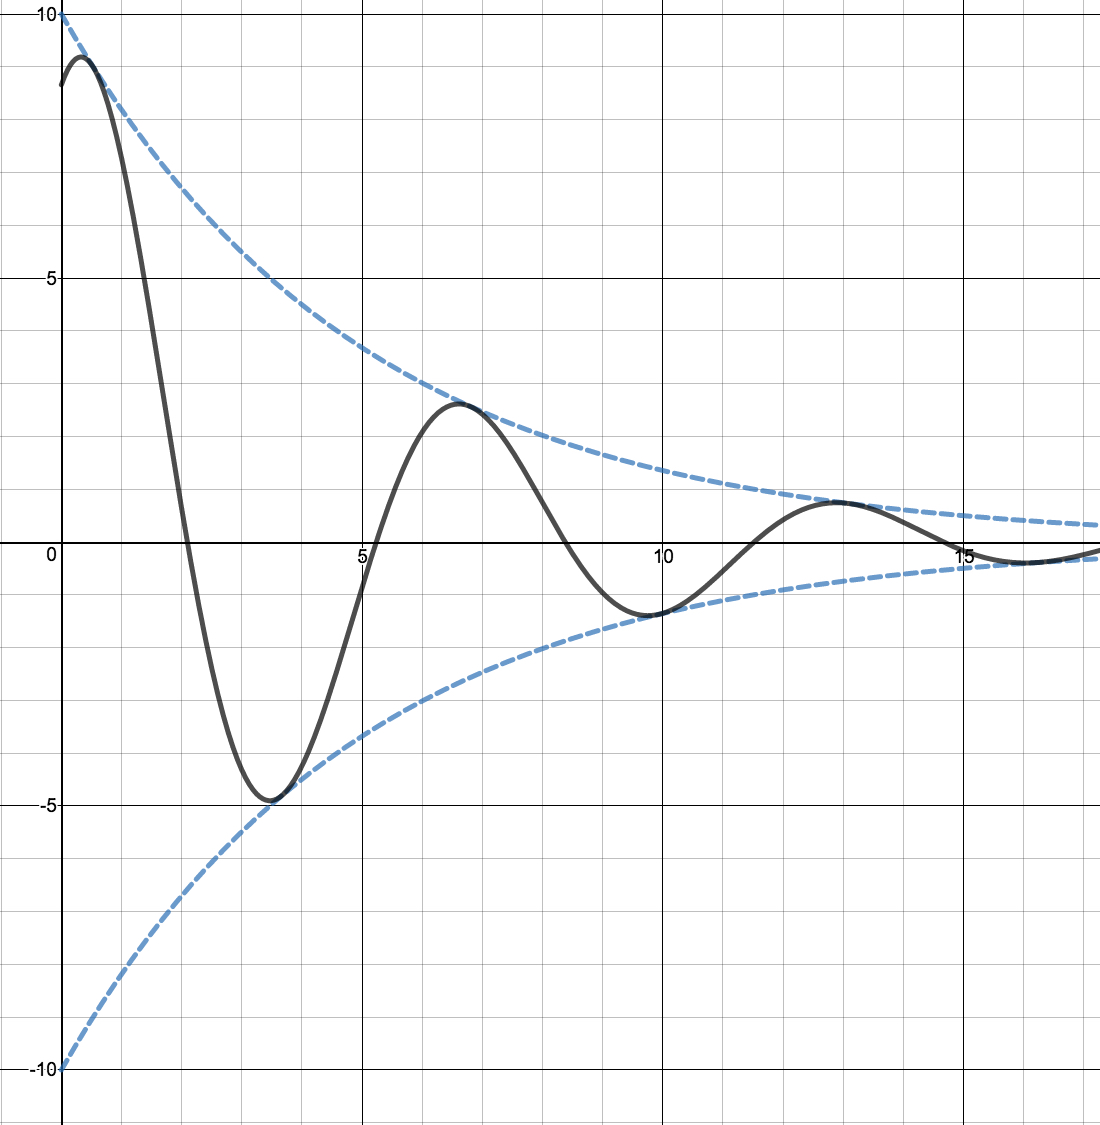
\includegraphics[height=2.5in]{./TrigonometricEquationsandInequalitiesGraphics/Sinusoid06.jpg} 

{\boldmath $x(t) = 10e^{-t/5} \sin\left(t + \frac{\pi}{3}\right)$} and $x= \pm 10e^{-t/5}$ \\

\end{center}

In this case, the function $x(t)$  corresponds to the motion of an object on a spring where there is a slight force which acts to `damp', or slow the motion.  An example of this kind of force would be the friction of the object against the air. According to  this model, the object oscillates forever, but with increasingly smaller and smaller amplitude.  This motion is often described as \index{underdamped}\index{harmonic motion ! underdamped}\index{motion ! underdamped}\textbf{underdamped} motion.


\item  Proceeding as in the first example, we factor out $(t+3)\sqrt{2}$ from each term in the function $x(t)$ to get $x(t) = (t+3)\sqrt{2}(\cos(2t) + \sin(2t))$.   We find $(\cos(2t) + \sin(2t)) = \sqrt{2} \sin\left(2t + \frac{\pi}{4}\right)$, so an equivalent form of $x(t)$ is  $x(t) = 2(t+3) \sin\left(2t + \frac{\pi}{4}\right)$.  

\smallskip

Graphing $x(t)$, we find the sinusoid's amplitude growing.  This isn't too surprising  since our amplitude function here is $A(t) = 2(t+3) = 2t+6$, grows without bound as $t \rightarrow \infty$.  


\begin{center}

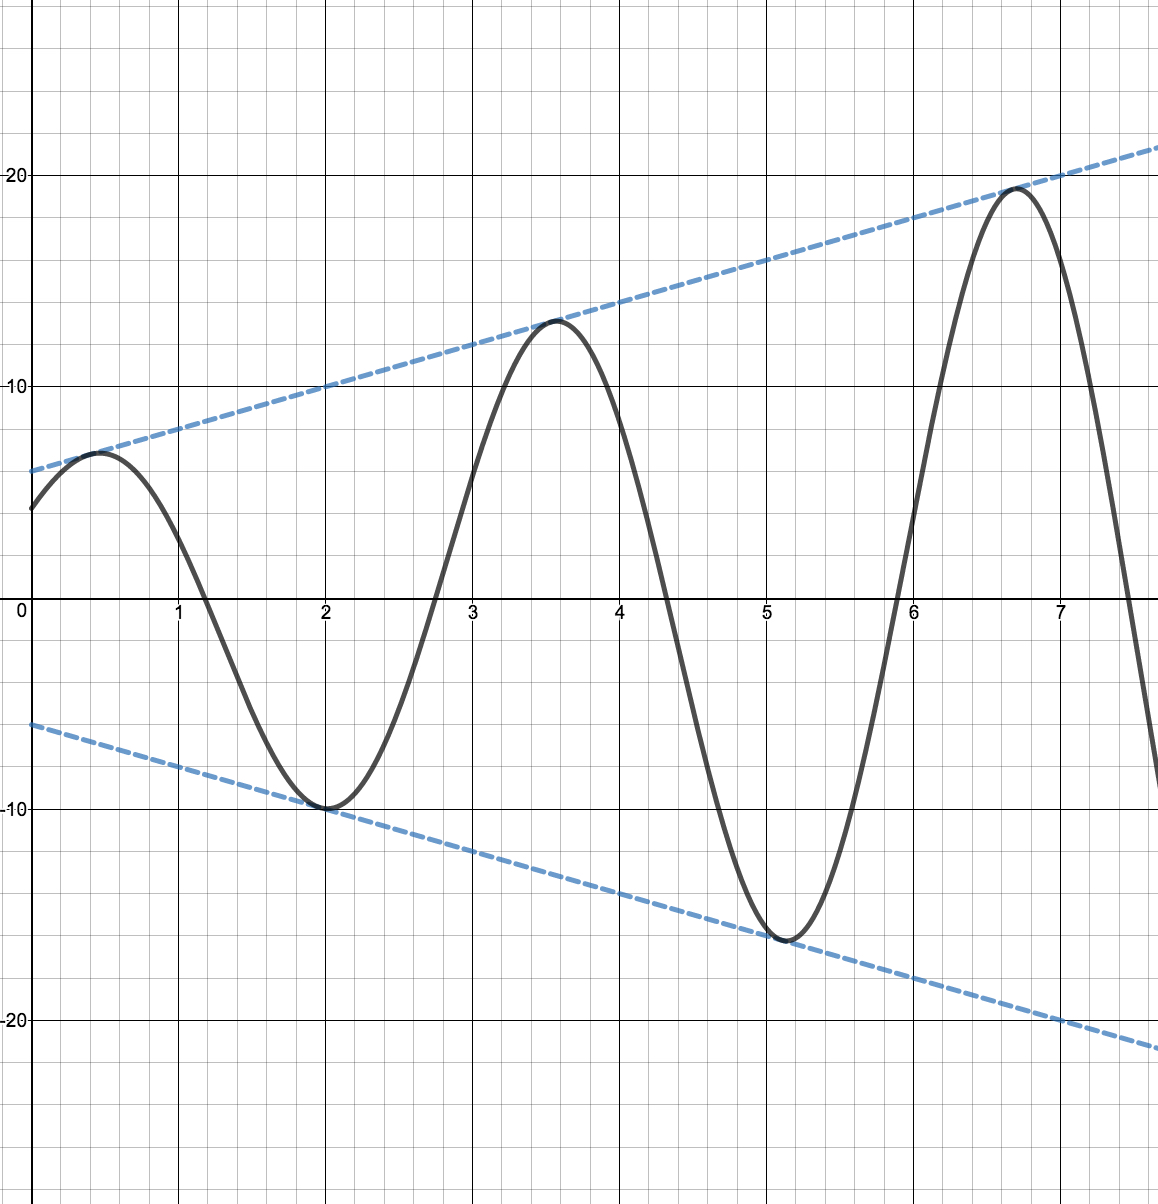
\includegraphics[height=2.5in]{./TrigonometricEquationsandInequalitiesGraphics/Sinusoid08.jpg} 

{\boldmath $x(t)= 2(t+3) \sin\left(2t + \frac{\pi}{4}\right)$} and $x = \pm 2(t+3)$ \\



\end{center}

The phenomenon illustrated here is `forced' motion.  That is, we imagine that the entire apparatus on which the spring is attached is oscillating as well.  

\smallskip

In this particular case, we are witnessing a `resonance' effect -- the frequency of the external oscillation matches the frequency of the motion of the object on the spring. In a mechanical system, this will result in some sort of structural failure.\footnote{The reader is invited to investigate the destructive implications of \href{http://en.wikipedia.org/wiki/Resonance}{\underline{resonance}}.}



\vspace{-.1in}

\item Last, but not least, we come to  $x(t) = 5\sin(6t) - 5\sin(8t)$.  To find the period of this function, we need to determine the length of the smallest interval on which both $f(t) = 5\sin(6t)$ and $g(t) = 5\sin(8t)$ complete a whole number of cycles. 

\smallskip

To do this, we take the ratio of their frequencies and reduce to lowest terms:  $\frac{6}{8} = \frac{3}{4}$.  This tells us that for every $3$ cycles $f$ makes, $g$ makes $4$. Hence,  the period of $x(t)$ is three times the period of $f(t)$ (which is four times the period of $g(t)$), or $\pi$.   We check our work by graphing $x(t)$  over  $[0,\pi]$

\smallskip

The reader may recognize $x(t)$  an example of the `beats' phenomenon we first saw on \pageref{beats} in Section \ref{expandedsinusoid}.  Indeed, using a sum to product identity, we may rewrite $x(t)$ as $x(t) =  -10 \sin(t) \cos(7t)$.  As we saw on \pageref{beats}  (and Exercises \ref{beatexfirst} - \ref{beatexlast} in Section \ref{MoreTrigonometricIdentities}), the lower frequency factor, $-10\sin(t)$ determines the `wave-envelope,'   $x = \pm 10 \sin(t)$.  


\begin{center}

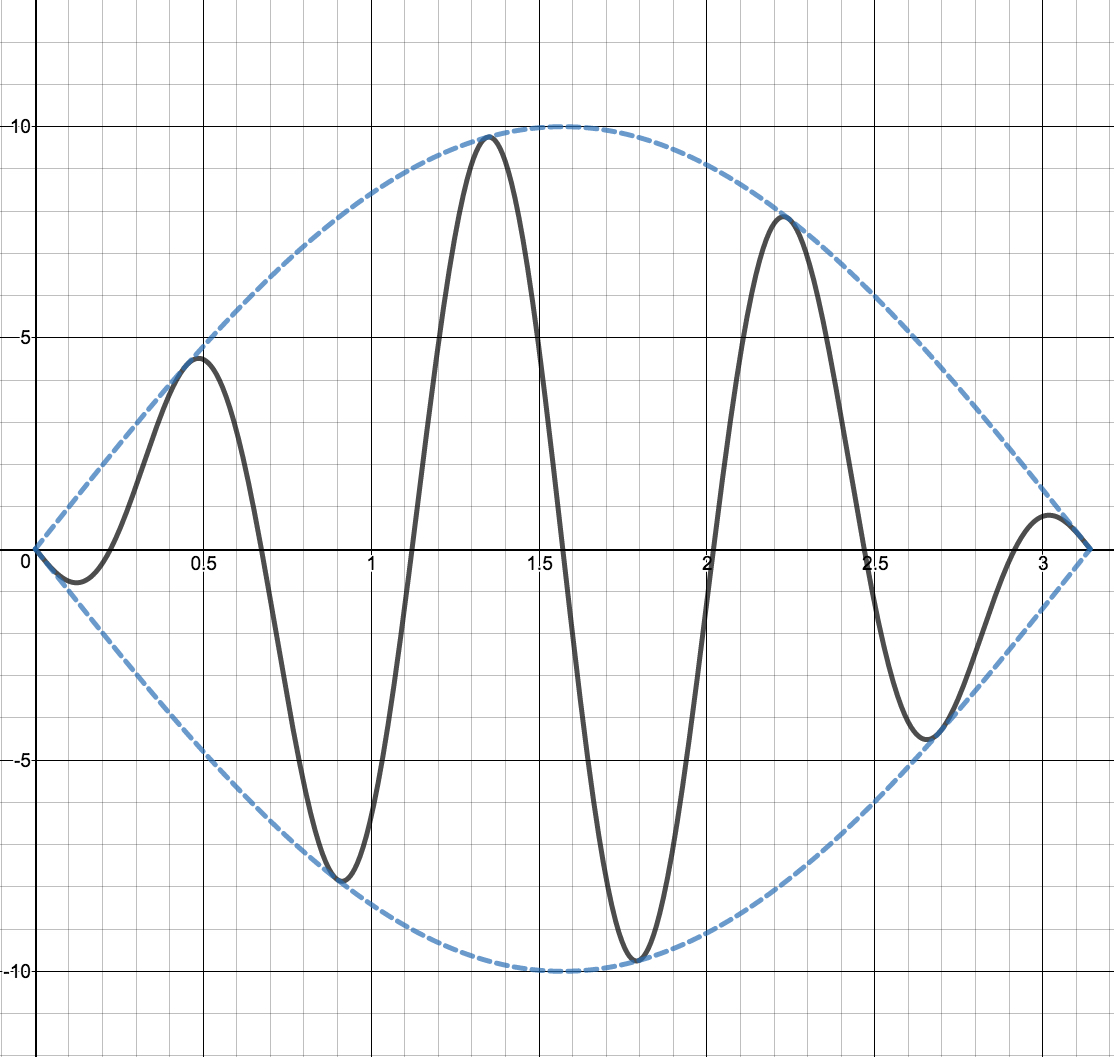
\includegraphics[height=2.5in]{./TrigonometricEquationsandInequalitiesGraphics/Sinusoid10.jpg} 


{\boldmath $x(t) = 5\sin(6t) - 5\sin(8t)$} and  $x = \pm 10 \sin(t)$ over $[0,\pi]$



\end{center}

 This equation of motion also results from `forced' motion, but here the frequency of the external oscillation is different than that of the object on the spring.  Since the sinusoids here have different frequencies, they are `out of sync' and  do not amplify each other as in the previous example.  Instead, through a combination of constructive and destructive interference, the mass continues to oscillate no more than $10$ units from its equilibrium position indefinitely.  \qed


\end{enumerate}

\end{example}

Our last examples use the tools of this section along with those developed in Section \ref{AppDerivatives}.

\begin{example}\label{sinecurvesketckex01}   Let $f(x) = 2 \sin(x) - \sin(2x)$ restricted to the interval $[0, 2\pi]$.

\begin{enumerate}

\item Given $f'(x) = 2 \cos(x) - 2\cos(2x)$,   find the open intervals over which $f$ is increasing and decreasing.

\item  Locate all relative extrema and check your answers graphically.

\end{enumerate}

{\bf Solution.}

\begin{enumerate}

\item We begin making a sign diagram for $f'(x) = 2 \cos(x) - 2\cos(2x)$ by  solving $f'(x) = 0$: 

\begin{longtable}{rclr}

$f'(x)$ & $=$ & $0$ & \\[8pt]

$2\cos(x) - 2\cos(2x)$ & $=$ & $0$ & \\[8pt]

$2\cos(x) - 2\left( 2 \cos^{2}(x) - 1 \right)$ & $=$ & $0$ &  \text{Double Angle Identity:  $\cos(2x) = 2 \cos^{2}(x) - 1$} \\[8pt]

$2\cos(x) - 4 \cos^{2}(x) + 2$ & $=$ & $0$ & \\[8pt]

$-2\left( 2 \cos^{2}(x) - \cos(x) -1 \right)$ &$ =$ & $0$ & \\[8pt]

$-2 ( 2\cos(x) +1) (\cos(x) -1)$ & $=$ & $0$ & \\  

\end{longtable}

We get $2\cos(x) + 1 = 0$ or $\cos(x) = -\frac{1}{2}$.  In the interval $(0, 2\pi)$, the only solutions are $x = \frac{2\pi}{3}$ and $x = \frac{4\pi}{3}$.  We also get $\cos(x) -1 = 0$ or $\cos(x) = 1$ which occurs at the endpoints $x = 0$ and $x = 2\pi$.

\smallskip

We create our sign diagram for $f'(x)$ and interpret what it means for $f(x)$ below.


\begin{center}

\begin{multicols}{2}

\begin{mfpic}[15]{-6}{6}{-2}{2}
 \polyline{(-5,0),(5,0)}
\xmarks{-5, -2,2, 5}
\arrow \polyline{(-3.5,-1.5),(-3.5,-0.5)}
\arrow \polyline{(0,-1.5),(0,-0.5)}
\arrow \polyline{(3.5,-1.5),(3.5,-0.5)}
\tlpointsep{4pt}
\axislabels {x}{{$\frac{2\pi}{3}$} -2, {$\frac{4\pi}{3}$} 2, {$0$} -5, {$2\pi$} 5}
\tlabel[cc](-3.5,1){$(+)$}
\tlabel[cc](-2,1){$0$}
\tlabel[cc](0,1){$(-)$}
\tlabel[cc](2,1){$0$}
\tlabel[cc](3.5,1){$(+)$}
\tlabel[cc](-3.5,-2.25){$\frac{\pi}{2}$}
\tlabel[cc](0,-2.25){$\pi$}
\tlabel[cc](3.5,-2.25){$\frac{3\pi}{2}$}
\tlabel[cc](6.5,1){$f'(x)$}
\tlabel[cc](6.5,-1){$x$}
\end{mfpic}

\begin{mfpic}[15]{-6}{6}{-2}{2}
 \polyline{(-5,0),(5,0)}
\xmarks{-5, -2,2, 5}
%\arrow \polyline{(-3.5,-1.5),(-3.5,-0.5)}
%\arrow \polyline{(0,-1.5),(0,-0.5)}
%\arrow \polyline{(3.5,-1.5),(3.5,-0.5)}
\tlpointsep{4pt}
\axislabels {x}{{$\frac{2\pi}{3}$} -2, {$\frac{4\pi}{3}$} 2, {$0$} -5, {$2\pi$} 5}
\tlabel[cc](-5,1){$\rightarrow$}
\tlabel[cc](-3.5,1){$\nearrow$}
\tlabel[cc](-2,1){$\rightarrow$}
\tlabel[cc](0,1){$\searrow$}
\tlabel[cc](2,1){$\rightarrow$}
\tlabel[cc](3.5,1){$\nearrow$}
\tlabel[cc](5,1){$\rightarrow$}
%\tlabel[cc](-3.75,-2.25){$-3$}
%\tlabel[cc](0,-2.25){$0$}
%\tlabel[cc](3.6,-2.25){$4$}
\tlabel[cc](6.5,1){$f(x)$}
\tlabel[cc](6.5,-1){$x$}
\end{mfpic}


\end{multicols}
\end{center}


We find  $f$ is increasing on $\left( 0, \frac{2\pi}{3} \right)$ and $\left(\frac{4\pi}{3} , 2 \pi \right)$ and $f$ is decreasing on $\left( \frac{2\pi}{3}, \frac{4\pi}{3} \right)$. 

\item  Using the sign diagram along with the First Derivative Test, Theorem \ref{firstderivatvetest}, we find that   $f$ has a local maximum: $\left( \frac{2\pi}{3}, f \left(\frac{2\pi}{3}\right) \right) = \left( \frac{2\pi}{3}, \frac{3 \sqrt{3}}{2}  \right)$ and a local minimum:$\left( \frac{4\pi}{3}, f \left(\frac{4\pi}{3}\right) \right) = \left( \frac{4\pi}{3}, -\frac{3 \sqrt{3}}{2}  \right)$.  Both of these extrema are absolute (global) as well as local.

\begin{center}

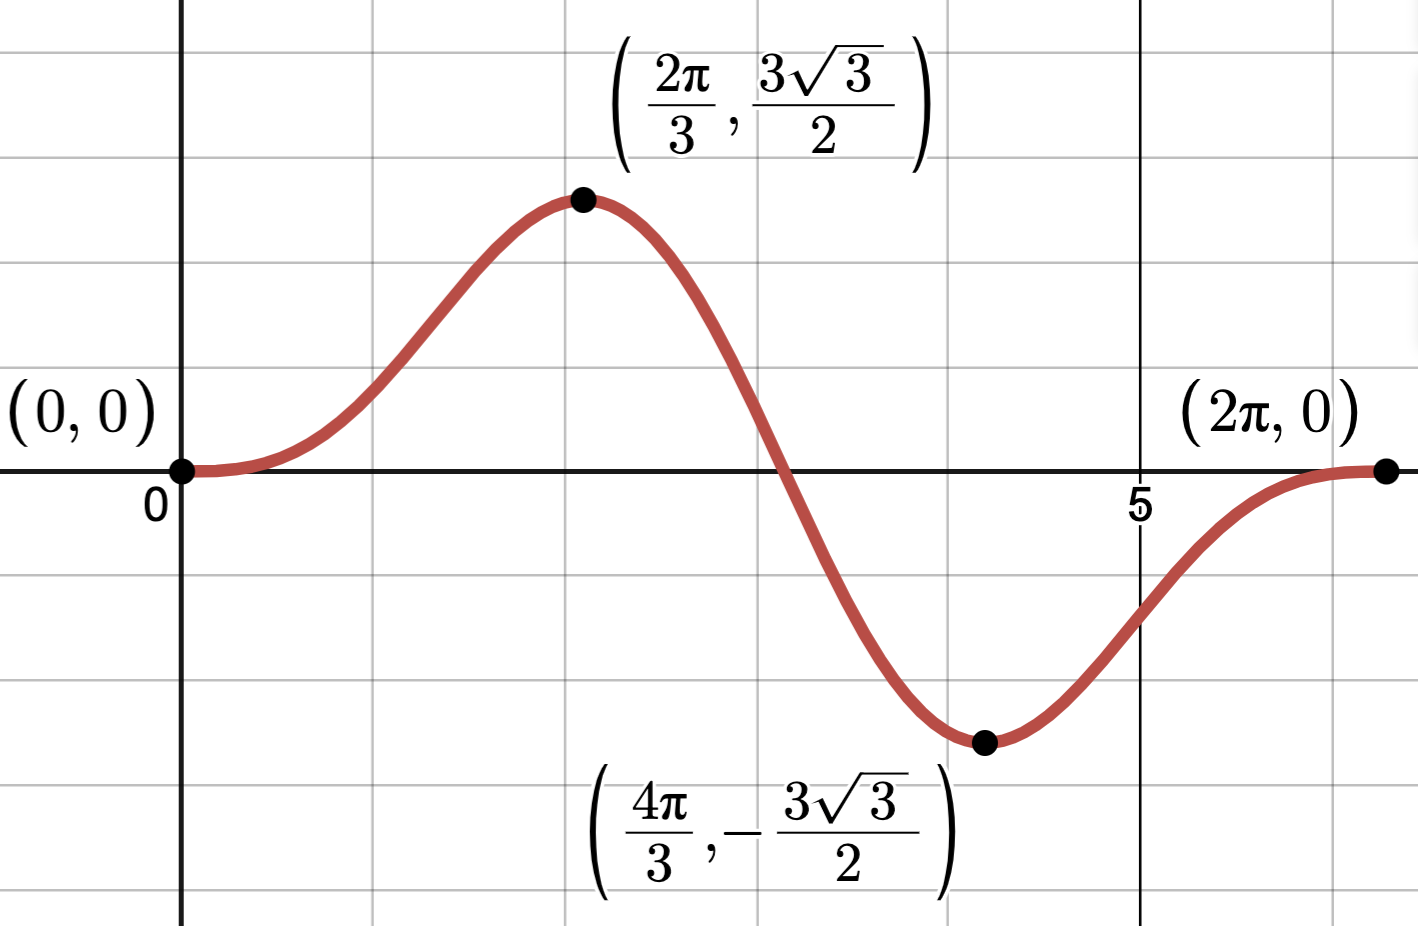
\includegraphics[width=4in]{./TrigonometricEquationsandInequalitiesGraphics/IncDecSine.png}

\end{center}

\hfill \qed

\end{enumerate}

\end{example}

We'll continue our work with $f(x) = 2 \sin(x) - \sin(2x)$ from Example \ref{sinecurvesketckex01} in Exercise \ref{sinecurvesketckex01IPs}.

\pagebreak

\begin{example}\label{IPexamplecosine}  Let  $f(x) = x-2\cos(x)$ restricted to the interval  $0 \leq x \leq 2\pi$.   

\medskip

 Given  $f''(x) = 2 \cos(x)$, find the inflection points of the graph.  Check your answer graphically.
 
 
 \medskip

{\bf Solution.}   We make a sign digram for $f''(x)$, first solving  $f''(x) = 2 \cos(x) = 0$.  We get $x = \frac{\pi}{2}$ and $x = \frac{3\pi}{2}$.  

 \medskip

\begin{center}

\begin{multicols}{2}

\begin{mfpic}[15]{-6}{6}{-2}{2}
 \polyline{(-5,0),(5,0)}
\xmarks{-5, -2,2, 5}
\arrow \polyline{(-3.5,-1.5),(-3.5,-0.5)}
\arrow \polyline{(0,-1.5),(0,-0.5)}
\arrow \polyline{(3.5,-1.5),(3.5,-0.5)}
\tlpointsep{4pt}
\axislabels {x}{{$\frac{\pi}{2}$} -2, {$\frac{3\pi}{2}$} 2, {$0$} -5, {$2\pi$} 5}
\tlabel[cc](-3.5,1){$(+)$}
\tlabel[cc](-2,1){$0$}
\tlabel[cc](0,1){$(-)$}
\tlabel[cc](2,1){$0$}
\tlabel[cc](3.5,1){$(+)$}
\tlabel[cc](-3.5,-2.25){$\frac{\pi}{3}$}
\tlabel[cc](0,-2.25){$\pi$}
\tlabel[cc](3.5,-2.25){$\frac{5\pi}{3}$}
\tlabel[cc](6.5,1){$f''(x)$}
\tlabel[cc](6.5,-1){$x$}
\end{mfpic}

\begin{mfpic}[15]{-6}{6}{-2}{2}
 \polyline{(-5,0),(5,0)}
\xmarks{-5, -2,2, 5}
%\arrow \polyline{(-3.5,-1.5),(-3.5,-0.5)}
%\arrow \polyline{(0,-1.5),(0,-0.5)}
%\arrow \polyline{(3.5,-1.5),(3.5,-0.5)}
\tlpointsep{4pt}
\axislabels {x}{{$\frac{\pi}{2}$} -2, {$\frac{3\pi}{2}$} 2, {$0$} -5, {$2\pi$} 5}
%\tlabel[cc](-5,1){$\rightarrow$}
\tlabel[cc](-3.5,1){\Huge $\smile$}
%\tlabel[cc](-2,1){$\rightarrow$}
\tlabel[cc](0,1){\Huge $\frown$}
%\tlabel[cc](2,1){$\rightarrow$}
\tlabel[cc](3.5,1){\Huge$\smile$}
%\tlabel[cc](5,1){$\rightarrow$}
%\tlabel[cc](-3.75,-2.25){$-3$}
%\tlabel[cc](0,-2.25){$0$}
%\tlabel[cc](3.6,-2.25){$4$}
\tlabel[cc](6.5,1){$f(x)$}
\tlabel[cc](6.5,-1){$x$}
\end{mfpic}


\end{multicols}
\end{center}

 \medskip

We see the concavity changes at both $x = \frac{\pi}{2}$ and $x = \frac{3\pi}{2}$ so we have inflection points:  $\left( \frac{\pi}{2}, f\left( \frac{\pi}{2} \right) \right) = \left( \frac{\pi}{2},\frac{\pi}{2} \right)$ and $\left( \frac{3\pi}{2}, f\left( \frac{3\pi}{2} \right) \right) = \left( \frac{3\pi}{2},\frac{3\pi}{2} \right)$.

 \medskip

\centerline{ 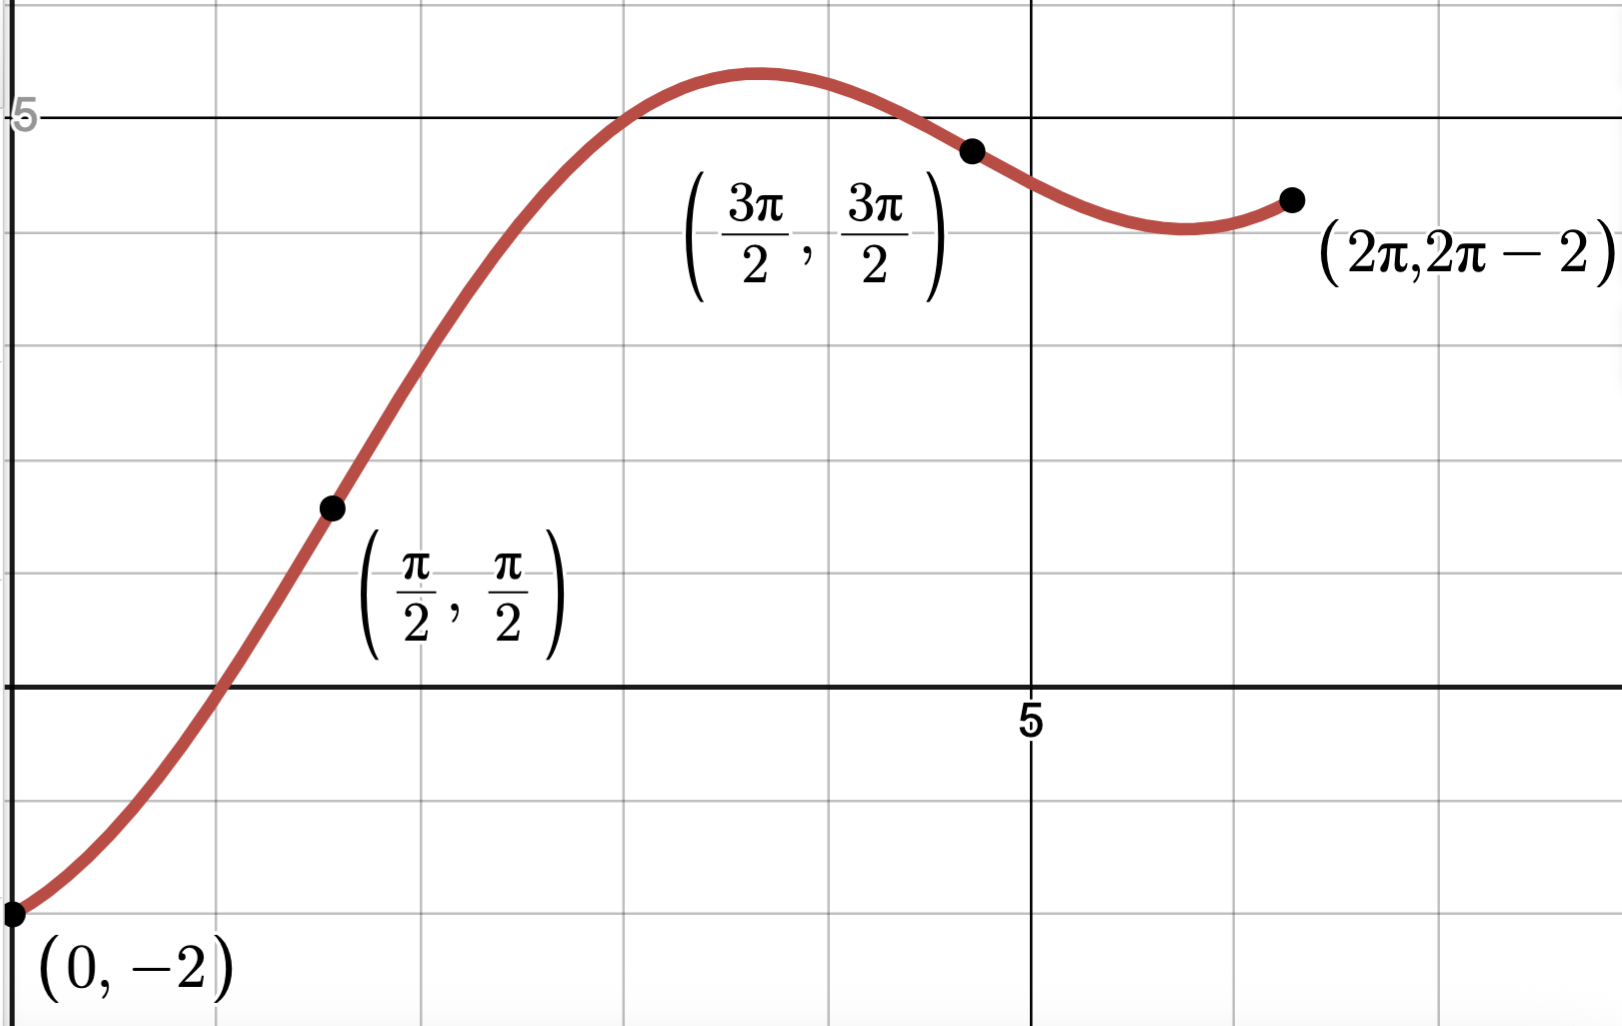
\includegraphics[width=4in]{./TrigonometricEquationsandInequalitiesGraphics/IPExample.png}}

\hfill \qed

\end{example}

We'll revisit  $f(x) = x-2\cos(x)$ from Example \ref{IPexamplecosine} in Exercise \ref{IPexamplecosineincdec}.  Speaking of Exercises \ldots

\newpage

\subsection{Exercises}
%% SKIPPED %% In Exercises \ref{solvebasicfirst} - \ref{solvebasiclast}, find \underline{all} of the exact solutions of the  equation and then list those solutions which are in the interval $[0, 2\pi)$.

\begin{multicols}{3}

\begin{enumerate}

\item $\sin \left( 5 \theta \right) = 0$ \vphantom{$\dfrac{\sqrt{3}}{2}$} \label{solvebasicfirst}
\item $\cos \left( 3t \right) = \dfrac{1}{2}$ \vphantom{$\dfrac{\sqrt{3}}{2}$}
\item $\sin \left( -2x \right) = \dfrac{\sqrt{3}}{2}$ 

\setcounter{HW}{\value{enumi}}

\end{enumerate}

\end{multicols}

\begin{multicols}{3}

\begin{enumerate}

\setcounter{enumi}{\value{HW}}

\item $\tan \left( 6 \theta \right) = 1$
\item $\csc \left( 4 t \right) = -1$
\item $\sec \left( 3x \right) = \sqrt{2}$

\setcounter{HW}{\value{enumi}}

\end{enumerate}

\end{multicols}

\begin{multicols}{3}

\begin{enumerate}

\setcounter{enumi}{\value{HW}}

\item $\cot \left( 2 \theta \right) = -\dfrac{\sqrt{3}}{3}$
\item $\cos \left( 9t  \right) = 9$ \vphantom{$\dfrac{\sqrt{3}}{2}$}
\item $\sin \left( \dfrac{x}{3} \right) = \dfrac{\sqrt{2}}{2}$

\setcounter{HW}{\value{enumi}}

\end{enumerate}

\end{multicols}

\begin{multicols}{3}

\begin{enumerate}

\setcounter{enumi}{\value{HW}}

\item $\cos \left( \theta+ \dfrac{5\pi}{6} \right) = 0$
\item $\sin \left( 2t - \dfrac{\pi}{3} \right) = -\dfrac{1}{2}$
\item $2\cos \left( x + \dfrac{7\pi}{4} \right) = \sqrt{3}$

\setcounter{HW}{\value{enumi}}

\end{enumerate}

\end{multicols}

\begin{multicols}{3}

\begin{enumerate}

\setcounter{enumi}{\value{HW}}

\item $\csc( \theta) = 0$
\item $\tan \left( 2t - \pi \right) = 1$
\item $\tan^{2} \left( x \right) = 3$

\setcounter{HW}{\value{enumi}}

\end{enumerate}

\end{multicols}

\begin{multicols}{3}

\begin{enumerate}

\setcounter{enumi}{\value{HW}}

\item $\sec^{2} \left( \theta \right) = \dfrac{4}{3}$
\item $\cos^{2} \left( t \right) = \dfrac{1}{2}$
\item $\sin^{2} \left( x \right) = \dfrac{3}{4}$ \label{solvebasiclast}

\setcounter{HW}{\value{enumi}}

\end{enumerate}

\end{multicols}

In Exercises \ref{solveidentfirst} - \ref{solveidentlast}, solve the equation, giving the exact solutions which lie in $[0, 2\pi)$


\begin{multicols}{2}

\begin{enumerate}

\setcounter{enumi}{\value{HW}}

\item $\sin \left( \theta \right) = \cos \left( \theta \right)$ \label{solveidentfirst}
\item $\sin \left( 2t \right) = \sin \left( t \right)$

\setcounter{HW}{\value{enumi}}

\end{enumerate}

\end{multicols}

\begin{multicols}{2}

\begin{enumerate}

\setcounter{enumi}{\value{HW}}

\item $\sin \left( 2x \right) = \cos \left( x \right)$
\item $\cos \left( 2\theta \right) = \sin \left( \theta \right)$

\setcounter{HW}{\value{enumi}}

\end{enumerate}

\end{multicols}

\begin{multicols}{2}

\begin{enumerate}

\setcounter{enumi}{\value{HW}}

\item $\cos \left( 2t \right) = \cos \left( t \right)$
\item  $\cos(2x) = 2 - 5\cos(x)$

\setcounter{HW}{\value{enumi}}

\end{enumerate}

\end{multicols}

\begin{multicols}{2}

\begin{enumerate}

\setcounter{enumi}{\value{HW}}

\item  $3\cos(2 \theta ) + \cos(\theta) + 2 = 0$
\item  $\cos(2t) = 5\sin(t) - 2$

\setcounter{HW}{\value{enumi}}

\end{enumerate}

\end{multicols}

\begin{multicols}{2}

\begin{enumerate}

\setcounter{enumi}{\value{HW}}

\item  $3\cos(2x) = \sin(x) + 2$
\item  $2\sec^{2}(\theta) = 3 - \tan(\theta)$

\setcounter{HW}{\value{enumi}}

\end{enumerate}

\end{multicols}

\begin{multicols}{2}

\begin{enumerate}

\setcounter{enumi}{\value{HW}}

\item  $\tan^{2}(t) = 1-\sec(t)$
\item  $\cot^{2}(x) = 3\csc(x) - 3$

\setcounter{HW}{\value{enumi}}

\end{enumerate}

\end{multicols}

\begin{multicols}{2}

\begin{enumerate}

\setcounter{enumi}{\value{HW}}

\item  $\sec(\theta) = 2\csc(\theta)$
\item  $\cos(t) \csc(t)\cot(t) = 6-\cot^{2}(t)$

\setcounter{HW}{\value{enumi}}

\end{enumerate}

\end{multicols}

\begin{multicols}{2}

\begin{enumerate}

\setcounter{enumi}{\value{HW}}

\item  $\sin(2x) = \tan(x)$
\item  $\cot^{4}(\theta) = 4\csc^{2}(\theta) - 7$

\setcounter{HW}{\value{enumi}}

\end{enumerate}

\end{multicols}

\begin{multicols}{2}

\begin{enumerate}

\setcounter{enumi}{\value{HW}}

\item  $\cos(2t) + \csc^{2}(t) = 0$
\item $\tan^{3} \left( x \right) = 3\tan \left( x \right)$

\setcounter{HW}{\value{enumi}}

\end{enumerate}

\end{multicols}

\begin{multicols}{2}

\begin{enumerate}

\setcounter{enumi}{\value{HW}}

\item $\tan^{2} \left( \theta \right) = \dfrac{3}{2} \sec \left( \theta \right)$
\item $\cos^{3} \left( t \right) = -\cos \left( t \right)$ \vphantom{$\dfrac{3}{2}$}

\setcounter{HW}{\value{enumi}}

\end{enumerate}

\end{multicols}

\begin{multicols}{2}

\begin{enumerate}

\setcounter{enumi}{\value{HW}}

\item $\tan (2x) - 2\cos(x) = 0$
\item $\csc^{3}(\theta) + \csc^{2}(\theta) = 4\csc(\theta) + 4$

\setcounter{HW}{\value{enumi}}

\end{enumerate}

\end{multicols}

\enlargethispage{0.35in}
\vspace{-0.15in}

\begin{multicols}{2}

\begin{enumerate}

\setcounter{enumi}{\value{HW}}

\item $2\tan(t) = 1 - \tan^{2}(t)$
\item $\tan \left( x \right) = \sec \left( x \right)$ \label{solveidentlast}

\setcounter{HW}{\value{enumi}}

\end{enumerate}

\end{multicols}

\pagebreak

In Exercises \ref{solvemoreidentfirst} - \ref{solvemoreidentlast}, solve the equation, giving the exact solutions which lie in $[0, 2\pi)$


\begin{multicols}{2}

\begin{enumerate}

\setcounter{enumi}{\value{HW}}

\item $\sin(6\theta) \cos(\theta) = -\cos(6\theta) \sin(\theta)$ \label{solvemoreidentfirst}
\item  $\sin(3t)\cos(t) = \cos(3t) \sin(t)$

\setcounter{HW}{\value{enumi}}

\end{enumerate}

\end{multicols}

\begin{multicols}{2}

\begin{enumerate}

\setcounter{enumi}{\value{HW}}

\item $\cos(2x)\cos(x) + \sin(2x)\sin(x) = 1$ \vphantom{$\dfrac{\sqrt{3}}{2}$}
\item \small $\cos(5\theta)\cos(3\theta) - \sin(5\theta)\sin(3\theta) = \dfrac{\sqrt{3}}{2}$ \normalsize

\setcounter{HW}{\value{enumi}}

\end{enumerate}

\end{multicols}

\begin{multicols}{2}

\begin{enumerate}

\setcounter{enumi}{\value{HW}}

%Sinusoids
\item $\sin(t) + \cos(t) = 1$
\item  $\sin(x) + \sqrt{3} \cos(x) = 1$

\setcounter{HW}{\value{enumi}}

\end{enumerate}

\end{multicols}

\begin{multicols}{2}

\begin{enumerate}

\setcounter{enumi}{\value{HW}}

\item  $\sqrt{2} \cos(\theta) - \sqrt{2} \sin(\theta) = 1$
\item  $\sqrt{3} \sin(2t) +  \cos(2t) = 1$

\setcounter{HW}{\value{enumi}}

\end{enumerate}

\end{multicols}

\begin{multicols}{2}

\begin{enumerate}

\setcounter{enumi}{\value{HW}}

\item $\cos(2x) - \sqrt{3} \sin(2x) = \sqrt{2}$
\item $3\sqrt{3}\sin(3\theta) - 3\cos(3\theta) = 3\sqrt{3}$

\setcounter{HW}{\value{enumi}}

\end{enumerate}

\end{multicols}

\begin{multicols}{2}

\begin{enumerate}

\setcounter{enumi}{\value{HW}}

\item  $\cos(3t) = \cos(5t)$
\item $\cos(4x) = \cos(2x)$

\setcounter{HW}{\value{enumi}}

\end{enumerate}

\end{multicols}

\begin{multicols}{2}

\begin{enumerate}

\setcounter{enumi}{\value{HW}}

\item $\sin(5\theta) = \sin(3\theta)$
\item $\cos(5t) = -\cos(2t)$

\setcounter{HW}{\value{enumi}}

\end{enumerate}

\end{multicols}

\begin{multicols}{2}
\begin{enumerate}
\setcounter{enumi}{\value{HW}}

\item $\sin(6x) + \sin(x) = 0$
\item $\tan(x) = \cos(x)$ \label{solvemoreidentlast}

\setcounter{HW}{\value{enumi}}
\end{enumerate}
\end{multicols}

In Exercises \ref{firstinveqn} - \ref{lastinveqn}, solve the equation.

\begin{multicols}{2}
\begin{enumerate}
\setcounter{enumi}{\value{HW}}

\item $\arccos(2x) = \pi$  \label{firstinveqn}  %Ans $x = -\frac{1}{2}$
\item $\pi - 2\arcsin(t) = 2\pi$   %Ans  $x=-1$

\setcounter{HW}{\value{enumi}}
\end{enumerate}
\end{multicols}

\begin{multicols}{2}
\begin{enumerate}
\setcounter{enumi}{\value{HW}}

\item $4\arctan(3x-1)-\pi=0$   %Ans $x = \frac{2}{3}$
\item $6 \, \text{arccot}(2t) - 5\pi = 0$   %Ans  $x=-\frac{\sqrt{3}}{2}$

\setcounter{HW}{\value{enumi}}
\end{enumerate}
\end{multicols}


\begin{multicols}{2}
\begin{enumerate}
\setcounter{enumi}{\value{HW}}

\item $4 \,\text{arcsec}\left(\frac{x}{2}\right) = \pi$   %Ans $x = 2\sqrt{2}$
\item $12 \,\text{arccsc}\left(\frac{t}{3}\right) = 2\pi$   %Ans $x = 6$

\setcounter{HW}{\value{enumi}}
\end{enumerate}
\end{multicols}

\begin{multicols}{2}
\begin{enumerate}
\setcounter{enumi}{\value{HW}}

\item $9 \arcsin^{2}(x) - \pi^2 = 0$   %Ans $x = \pm \frac{\sqrt{3}}{2}$
\item $9 \arccos^{2}(t) - \pi^2 = 0$   %Ans $x = \frac{1}{2}$

\setcounter{HW}{\value{enumi}}
\end{enumerate}
\end{multicols}

\begin{multicols}{2}
\begin{enumerate}
\setcounter{enumi}{\value{HW}}

\item $8 \, \text{arccot}^{2}(x)+3\pi^2=10 \pi \, \text{arccot}(x)$   %Ans $x = -1,0$
\item $6 \arctan(t)^2= \pi \arctan(x)+\pi^2$  \label{lastinveqn}  %Ans $x = -\sqrt{3}$

\setcounter{HW}{\value{enumi}}
\end{enumerate}
\end{multicols}


In Exercises \ref{firstineqfirst} - \ref{firstineqlast}, solve the inequality.  Express the exact answer in \underline{interval} notation, restricting your attention to $0 \leq x \leq 2\pi$.

\begin{multicols}{3}

\begin{enumerate}

\setcounter{enumi}{\value{HW}}

\item $\sin \left( x \right) \leq 0$ \label{firstineqfirst}
\item $\tan \left( t \right) \geq \sqrt{3}$
\item $\sec^{2} \left( x \right) \leq 4$

\setcounter{HW}{\value{enumi}}

\end{enumerate}

\end{multicols}

\begin{multicols}{3}

\begin{enumerate}

\setcounter{enumi}{\value{HW}}

\item $\cos^{2} \left( t \right) > \dfrac{1}{2}$
\item $\cos \left( 2x \right) \leq 0$ \vphantom{$\dfrac{1}{2}$}
\item $\sin \left( t + \dfrac{\pi}{3} \right) > \dfrac{1}{2}$

\setcounter{HW}{\value{enumi}}

\end{enumerate}

\end{multicols}

\begin{multicols}{3}

\begin{enumerate}

\setcounter{enumi}{\value{HW}}

\item $\cot^{2} \left( x \right) \geq \dfrac{1}{3}$
\item $2\cos(t) \geq 1$ \vphantom{$\dfrac{1}{2}$}
\item $\sin(5x) \geq 5$ \vphantom{$\dfrac{1}{2}$}

\setcounter{HW}{\value{enumi}}

\end{enumerate}

\end{multicols}

\begin{multicols}{3}

\begin{enumerate}

\setcounter{enumi}{\value{HW}}

\item $\cos(3t) \leq 1$
\item $\sec(x) \leq \sqrt{2}$
\item $\cot(t) \leq 4$ \label{firstineqlast}

\setcounter{HW}{\value{enumi}}
\end{enumerate}
\end{multicols}

\pagebreak

In Exercises \ref{secondineqefirst} - \ref{secondineqlast}, solve the inequality.  Express the exact answer in \underline{interval} notation, restricting your attention to $-\pi \leq x \leq \pi$.

\begin{multicols}{3}

\begin{enumerate}

\setcounter{enumi}{\value{HW}}

\item $\cos \left( x \right) > \dfrac{\sqrt{3}}{2}$ \label{secondineqefirst}
\item  $\sin(t) > \dfrac{1}{3}$ \vphantom{$\dfrac{\sqrt{3}}{2}$}
\item $\sec \left( x \right) \leq 2$ \vphantom{$\dfrac{\sqrt{3}}{2}$}

\setcounter{HW}{\value{enumi}}

\end{enumerate}

\end{multicols}

\begin{multicols}{3}

\begin{enumerate}

\setcounter{enumi}{\value{HW}}

\item $\sin^{2} \left( t \right) < \dfrac{3}{4}$
\item $\cot \left( x \right) \geq -1$ \vphantom{$\dfrac{1}{2}$}
\item $\cos(t) \geq \sin(t)$ \vphantom{$\dfrac{1}{2}$} \label{secondineqlast}

\setcounter{HW}{\value{enumi}}

\end{enumerate}

\end{multicols}

%\pagebreak

In Exercises \ref{thirdineqfirst} - \ref{thirdineqlast}, solve the inequality.  Express the exact answer in \underline{interval} notation, restricting your attention to $-2\pi \leq x \leq 2\pi$.

\begin{multicols}{3}

\begin{enumerate}

\setcounter{enumi}{\value{HW}}

\item $\csc \left( x \right) > 1$ \vphantom{$\dfrac{1}{2}$} \label{thirdineqfirst}
\item  $\cos(t) \leq \dfrac{5}{3}$
\item  $\cot(x) \geq 5$ \vphantom{$\dfrac{1}{2}$}

\setcounter{HW}{\value{enumi}}

\end{enumerate}

\end{multicols}

\begin{multicols}{3}

\begin{enumerate}

\setcounter{enumi}{\value{HW}}

\item $\tan^{2} \left( t \right) \geq 1$
\item $\sin(2x) \geq \sin(x)$
\item $\cos(2t) \leq \sin(x)$ \label{thirdineqlast}

\setcounter{HW}{\value{enumi}}

\end{enumerate}

\end{multicols}

In Exercises \ref{invineqfirst} - \ref{invineqlast}, solve the given inequality.

\begin{multicols}{4}

\begin{enumerate}

\setcounter{enumi}{\value{HW}}

\item $\arcsin(2x) > 0$ \label{invineqfirst}  
\item $3 \arccos(t) \leq \pi$
\item $6 \, \text{arccot}(7x) \geq \pi$  
\item $\pi > 2\arctan(t)$ 

\setcounter{HW}{\value{enumi}}

\end{enumerate}

\end{multicols}

\begin{multicols}{2}

\begin{enumerate}

\setcounter{enumi}{\value{HW}}

\item $2\arcsin(x)^2 > \pi \arcsin(x)$  
\item $12 \arccos(t)^2+2\pi^2>11\pi \arccos(t)$ \label{invineqlast} 

\setcounter{HW}{\value{enumi}}

\end{enumerate}

\end{multicols}

In Exercises \ref{domainfirst} - \ref{domainlast}, express the domain of the function using the extended interval notation. (See Example \ref{TrigDomainEx1} and Section \ref{extendedinterval} for details.)

\begin{multicols}{3}

\begin{enumerate}

\setcounter{enumi}{\value{HW}}

\item $f(x) = \dfrac{1}{\cos(x) - 1}$ \vphantom{$\dfrac{\cos(x)}{\sin(x) + 1}$} \label{domainfirst}
\item $f(t) = \dfrac{\cos(t)}{\sin(t) + 1}$
\item $f(x) = \sqrt{\tan^{2}(x) - 1}$ \vphantom{$\dfrac{\cos(x)}{\sin(x) + 1}$}

\setcounter{HW}{\value{enumi}}

\end{enumerate}

\end{multicols}

\begin{multicols}{3}

\begin{enumerate}

\setcounter{enumi}{\value{HW}}

\item $f(t) = \sqrt{2 - \sec(t)}$ \vphantom{$\dfrac{\cos(t)}{\sin(t) + 1}$}
\item $f(x) = \csc(2x)$ \vphantom{$\dfrac{\cos(x)}{\sin(x) + 1}$}
\item $f(t) = \dfrac{\sin(t)}{2 + \cos(t)}$

\setcounter{HW}{\value{enumi}}

\end{enumerate}

\end{multicols}

\begin{multicols}{3}

\begin{enumerate}

\setcounter{enumi}{\value{HW}}

\item $f(x) = 3\csc(x) + 4\sec(x)$ 
\item $f(t) = \ln\left( |\cos(t)| \right)$
\item $f(x) = \arcsin(\tan(x))$ \label{domainlast}

\setcounter{HW}{\value{enumi}}

\end{enumerate}

\end{multicols}

\begin{enumerate}

\setcounter{enumi}{\value{HW}}

\item \label{frequencynumberconnection} \begin{enumerate}

\item With the help of your classmates, determine the number of solutions to $\sin(x) = \frac{1}{2}$ in $[0,2\pi)$.  Then find the number of solutions to $\sin(2x) = \frac{1}{2}$,  $\sin(3x) = \frac{1}{2}$ and $\sin(4x) = \frac{1}{2}$ in $[0,2\pi)$. What pattern emerges?   Explain how this pattern would help you solve equations like $\sin(11x) = \frac{1}{2}$.  

\item Repeat the above exercise focusing on  $\sin\left(\frac{x}{2}\right)  = \frac{1}{2}$,  $\sin\left(\frac{3x}{2}\right)  = \frac{1}{2}$ and $\sin\left(\frac{5x}{2}\right)  = \frac{1}{2}$.  What pattern emerges here?  

\item  Replace sine with tangent and $\frac{1}{2}$ with $1$ and repeat the whole exploration.

\end{enumerate}

\setcounter{HW}{\value{enumi}}

\end{enumerate}

\pagebreak

\begin{enumerate}

\setcounter{enumi}{\value{HW}}
\item  Suppose an object weighing $10$ pounds is suspended from the ceiling by a spring which stretches $2$ feet to its equilibrium position when the object is attached.  

\begin{enumerate}

\item  Find the spring constant $k$ in $\frac{\text{lbs.}}{\text{ft.}}$ and the mass of the object in slugs.
\item  Find the equation of motion of the object if it is released from $1$ foot \textit{below} the equilibrium position from rest.  When is the first time the object passes through the equilibrium position? In which direction is it heading?
\item  Find the equation of motion of the object if it is released from $6$ inches \textit{above} the equilibrium position with a \textit{downward} velocity of $2$ feet per second.  Find when the object passes through the equilibrium position heading downwards for the third time.


\end{enumerate}

\setcounter{HW}{\value{enumi}}

\item\label{sinecurvesketckex01IPs} In Example \ref{sinecurvesketckex01},  $f(x) = 2\sin(x) - \sin(2x)$  restricted to $0 \leq x \leq 2\pi$.  If $f''(x) = 4 \sin(2x) - 2\sin(x)$,  find the inflection points of the graph of $y = f(x)$. 

\item\label{IPexamplecosineincdec} In Example \ref{IPexamplecosine},  $f(x) =x-2\cos(x)$ restricted to $0 \leq x \leq 2\pi$.  If $f'(x) = 2\sin(x)+1$, list the open intervals over which $f$ is increasing and decreasing.  Find the local extrema. 



\item\label{squeezefordampedmotionexercise} Recall  $x(t) = 10e^{-t/5} \sin\left(t + \frac{\pi}{3}\right)$ from  Example \ref{underdampedresonance} number \ref{underdampedproblem} models underdamped motion. Use the Squeeze Theorem, Theorem \ref{squeezeth}, to prove $\ds{\lim_{t \rightarrow \infty} x(t) = 0}$.

\smallskip

\textbf{HINT:}  Since $-1 \leq \sin\left(t + \frac{\pi}{3}\right) \leq 1$, $-10e^{-t/5} \leq   10e^{-t/5} \sin\left(t + \frac{\pi}{3}\right) \leq 10e^{-t/5}$ \ldots


\end{enumerate}

\newpage

\subsection{Answers}

\begin{enumerate}

\item $\theta = \dfrac{\pi k}{5}; \; \theta = 0, \dfrac{\pi}{5}, \dfrac{2\pi}{5}, \dfrac{3\pi}{5}, \dfrac{4\pi}{5}, \pi, \dfrac{6\pi}{5}, \dfrac{7\pi}{5}, \dfrac{8\pi}{5}, \dfrac{9\pi}{5}$

\item $t  = \dfrac{\pi}{9} + \dfrac{2\pi k}{3}$ or $t = \dfrac{5\pi}{9} + \dfrac{2\pi k}{3}; \; t = \dfrac{\pi}{9}, \dfrac{5\pi}{9}, \dfrac{7\pi}{9}, \dfrac{11\pi}{9}, \dfrac{13\pi}{9}, \dfrac{17\pi}{9}$

\item $x = \dfrac{2\pi}{3} + \pi k$ or $x = \dfrac{5\pi}{6} + \pi k; \; x = \dfrac{2\pi}{3}, \dfrac{5\pi}{6}, \dfrac{5\pi}{3}, \dfrac{11\pi}{6}$

\item $\theta = \dfrac{\pi}{24} + \dfrac{\pi k}{6}; \; \theta = \dfrac{\pi}{24}, \dfrac{5\pi}{24}, \dfrac{3\pi}{8}, \dfrac{13\pi}{24}, \dfrac{17\pi}{24}, \dfrac{7\pi}{8}, \dfrac{25\pi}{24}, \dfrac{29\pi}{24}, \dfrac{11\pi}{8}, \dfrac{37\pi}{24}, \dfrac{41\pi}{24}, \dfrac{15\pi}{8}$

\item $t = \dfrac{3\pi}{8} + \dfrac{\pi k}{2}; \; t = \dfrac{3\pi}{8}, \dfrac{7\pi}{8}, \dfrac{11\pi}{8}, \dfrac{15\pi}{8}$

\item $x = \dfrac{\pi}{12} + \dfrac{2\pi k}{3}$ or $x = \dfrac{7\pi}{12} + \dfrac{2\pi k}{3}; \; x = \dfrac{\pi}{12}, \dfrac{7\pi}{12}, \dfrac{3\pi}{4}, \dfrac{5\pi}{4}, \dfrac{17\pi}{12}, \dfrac{23\pi}{12}$

\item $\theta  = \dfrac{\pi}{3} + \dfrac{\pi k}{2}; \; \theta  = \dfrac{\pi}{3}, \dfrac{5\pi}{6}, \dfrac{4\pi}{3}, \dfrac{11\pi}{6}$

\item No solution

\item $x = \dfrac{3\pi}{4} + 6\pi k$ or $x = \dfrac{9\pi}{4} + 6\pi k; \; x = \dfrac{3\pi}{4}$

\item $\theta = -\dfrac{\pi}{3} + \pi k; \; \theta  = \dfrac{2\pi}{3}, \dfrac{5\pi}{3}$

\item $t = \dfrac{3\pi}{4} + \pi k$ or $t = \dfrac{13\pi}{12} + \pi k; \; t = \dfrac{\pi}{12}, \dfrac{3\pi}{4}, \dfrac{13\pi}{12}, \dfrac{7\pi}{4}$

\item $x = -\dfrac{19\pi}{12} + 2\pi k$ or $x = \dfrac{\pi}{12} + 2\pi k; \; x = \dfrac{\pi}{12}, \dfrac{5\pi}{12}$

\item No solution

\item $t = \dfrac{5\pi}{8} + \dfrac{\pi k}{2}; \; t = \dfrac{\pi}{8}, \dfrac{5\pi}{8}, \dfrac{9\pi}{8}, \dfrac{13\pi}{8}$

\item $x = \dfrac{\pi}{3} + \pi k$ or $x = \dfrac{2\pi}{3} + \pi k; \; x = \dfrac{\pi}{3}, \dfrac{2\pi}{3}, \dfrac{4\pi}{3}, \dfrac{5\pi}{3}$

\item $\theta  = \dfrac{\pi}{6} + \pi k$ or $\theta = \dfrac{5\pi}{6} + \pi k; \; \theta = \dfrac{\pi}{6}, \dfrac{5\pi}{6}, \dfrac{7\pi}{6}, \dfrac{11\pi}{6}$

\item $t = \dfrac{\pi}{4} + \dfrac{\pi k}{2}; \; t = \dfrac{\pi}{4}, \dfrac{3\pi}{4}, \dfrac{5\pi}{4}, \dfrac{7\pi}{4}$

\item $x = \dfrac{\pi}{3} + \pi k$ or $x = \dfrac{2\pi}{3} + \pi k; \; x = \dfrac{\pi}{3}, \dfrac{2\pi}{3}, \dfrac{4\pi}{3}, \dfrac{5\pi}{3}$

\setcounter{HW}{\value{enumi}}

\end{enumerate}

\begin{multicols}{2}

\begin{enumerate}

\setcounter{enumi}{\value{HW}}

\item $\theta = \dfrac{\pi}{4}, \dfrac{5\pi}{4}$
\item $t = 0, \dfrac{\pi}{3}, \pi, \dfrac{5\pi}{3}$

\setcounter{HW}{\value{enumi}}

\end{enumerate}

\end{multicols}

\begin{multicols}{2}

\begin{enumerate}

\setcounter{enumi}{\value{HW}}

\item $x = \dfrac{\pi}{6}, \dfrac{\pi}{2}, \dfrac{5\pi}{6}, \dfrac{3\pi}{2}$
\item $\theta = \dfrac{\pi}{6}, \dfrac{5\pi}{6}, \dfrac{3\pi}{2}$

\setcounter{HW}{\value{enumi}}

\end{enumerate}

\end{multicols}

\begin{multicols}{2}

\begin{enumerate}

\setcounter{enumi}{\value{HW}}

\item $t = 0, \dfrac{2\pi}{3}, \dfrac{4\pi}{3}$
\item  $x=\dfrac{\pi}{3}, \dfrac{5\pi}{3}$

\setcounter{HW}{\value{enumi}}

\end{enumerate}

\end{multicols}

\begin{multicols}{2}

\begin{enumerate}

\setcounter{enumi}{\value{HW}}

\item  $\theta = \dfrac{2\pi}{3}, \dfrac{4\pi}{3}, \arccos\left(\dfrac{1}{3}\right), 2\pi -\arccos\left(\dfrac{1}{3}\right) $
\item  $t=\dfrac{\pi}{6}, \dfrac{5\pi}{6}$

\setcounter{HW}{\value{enumi}}

\end{enumerate}

\end{multicols}

\begin{multicols}{2}

\begin{enumerate}

\setcounter{enumi}{\value{HW}}

\item  $x = \dfrac{7\pi}{6}, \dfrac{11\pi}{6}, \arcsin\left(\dfrac{1}{3}\right), \pi - \arcsin\left(\dfrac{1}{3}\right) $
\item  $\theta=\dfrac{3\pi}{4}, \dfrac{7\pi}{4}, \arctan\left(\dfrac{1}{2}\right), \pi +\arctan\left(\dfrac{1}{2}\right) $

\setcounter{HW}{\value{enumi}}

\end{enumerate}

\end{multicols}

\begin{multicols}{2}

\begin{enumerate}

\setcounter{enumi}{\value{HW}}

\item  $t=0, \dfrac{2\pi}{3}, \dfrac{4\pi}{3}$
\item  $x=\dfrac{\pi}{6}, \dfrac{5\pi}{6}, \dfrac{\pi}{2}$

\setcounter{HW}{\value{enumi}}

\end{enumerate}

\end{multicols}

\begin{multicols}{2}

\begin{enumerate}

\setcounter{enumi}{\value{HW}}

\item  $\theta=\arctan(2), \pi + \arctan(2)$ \vphantom{$\dfrac{7\pi}{6}$}
\item  $t = \dfrac{\pi}{6}, \dfrac{7\pi}{6}, \dfrac{5\pi}{6}, \dfrac{11\pi}{6}$

\setcounter{HW}{\value{enumi}}

\end{enumerate}

\end{multicols}

\begin{multicols}{2}

\begin{enumerate}

\setcounter{enumi}{\value{HW}}

\item  $x = 0, \pi, \dfrac{\pi}{4}, \dfrac{3\pi}{4}, \dfrac{5\pi}{4}, \dfrac{7\pi}{4}$
\item  $\theta = \dfrac{\pi}{6}, \dfrac{\pi}{4}, \dfrac{3\pi}{4}, \dfrac{5\pi}{6}, \dfrac{7\pi}{6}, \dfrac{5\pi}{4}, \dfrac{7\pi}{4}, \dfrac{11\pi}{6}$

\setcounter{HW}{\value{enumi}}

\end{enumerate}

\end{multicols}

\begin{multicols}{2}

\begin{enumerate}

\setcounter{enumi}{\value{HW}}

\item  $t = \dfrac{\pi}{2}, \dfrac{3\pi}{2}$
\item $x = 0, \dfrac{\pi}{3}, \dfrac{2\pi}{3}, \pi, \dfrac{4\pi}{3}, \dfrac{5\pi}{3}$

\setcounter{HW}{\value{enumi}}

\end{enumerate}

\end{multicols}

\begin{multicols}{2}

\begin{enumerate}

\setcounter{enumi}{\value{HW}}

\item $\theta  = \dfrac{\pi}{3}, \dfrac{5\pi}{3}$
\item $t = \dfrac{\pi}{2}, \dfrac{3\pi}{2}$

\setcounter{HW}{\value{enumi}}

\end{enumerate}

\end{multicols}

\begin{multicols}{2}

\begin{enumerate}

\setcounter{enumi}{\value{HW}}

\item $x = \dfrac{\pi}{6}, \dfrac{\pi}{2}, \dfrac{5\pi}{6}, \dfrac{3\pi}{2}$
\item $\theta = \dfrac{\pi}{6}, \dfrac{5\pi}{6}, \dfrac{7\pi}{6}, \dfrac{3\pi}{2}, \dfrac{11\pi}{6}$

\setcounter{HW}{\value{enumi}}

\end{enumerate}

\end{multicols}

\begin{multicols}{2}

\begin{enumerate}

\setcounter{enumi}{\value{HW}}

\item $t = \dfrac{\pi}{8}, \dfrac{5\pi}{8}, \dfrac{9\pi}{8}, \dfrac{13\pi}{8}$
\item No solution \vphantom{$\dfrac{7\pi}{6}$}

\setcounter{HW}{\value{enumi}}

\end{enumerate}

\end{multicols}

\begin{enumerate}

\setcounter{enumi}{\value{HW}}

\item $\theta = 0, \dfrac{\pi}{7}, \dfrac{2\pi}{7}, \dfrac{3\pi}{7}, \dfrac{4\pi}{7}, \dfrac{5\pi}{7}, \dfrac{6\pi}{7}, \pi, \dfrac{8\pi}{7}, \dfrac{9\pi}{7}, \dfrac{10\pi}{7}, \dfrac{11\pi}{7}, \dfrac{12\pi}{7}, \dfrac{13\pi}{7}$

\setcounter{HW}{\value{enumi}}

\end{enumerate}

\begin{multicols}{2}

\begin{enumerate}

\setcounter{enumi}{\value{HW}}

\item  $t=0, \dfrac{\pi}{2}, \pi, \dfrac{3\pi}{2}$

\item $x = 0$ \vphantom{$\dfrac{7\pi}{6}$}

\setcounter{HW}{\value{enumi}}

\end{enumerate}

\end{multicols}

\begin{enumerate}

\setcounter{enumi}{\value{HW}}

\item $\theta = \dfrac{\pi}{48}, \dfrac{11\pi}{48}, \dfrac{13\pi}{48}, \dfrac{23\pi}{48}, \dfrac{25\pi}{48}, \dfrac{35\pi}{48}, \dfrac{37\pi}{48}, \dfrac{47\pi}{48}, \dfrac{49\pi}{48}, \dfrac{59\pi}{48}, \dfrac{61\pi}{48}, \dfrac{71\pi}{48}, \dfrac{73\pi}{48}, \dfrac{83\pi}{48}, \dfrac{85\pi}{48}, \dfrac{95\pi}{48}$

\setcounter{HW}{\value{enumi}}

\end{enumerate}

\begin{multicols}{2}

\begin{enumerate}

\setcounter{enumi}{\value{HW}}

\item $t = 0, \dfrac{\pi}{2}$ \vphantom{$\dfrac{7\pi}{6}$}
\item  $x = \dfrac{\pi}{2}, \dfrac{11\pi}{6}$

\setcounter{HW}{\value{enumi}}

\end{enumerate}

\end{multicols}

\begin{multicols}{2}

\begin{enumerate}

\setcounter{enumi}{\value{HW}}

\item  $\theta = \dfrac{\pi}{12}, \dfrac{17\pi}{12}$
\item  $t = 0, \pi, \dfrac{\pi}{3}, \dfrac{4\pi}{3}$

\setcounter{HW}{\value{enumi}}

\end{enumerate}

\end{multicols}

\begin{multicols}{2}

\begin{enumerate}

\setcounter{enumi}{\value{HW}}

\item  $x = \dfrac{17 \pi}{24}, \dfrac{41 \pi}{24}, \dfrac{23\pi}{24}, \dfrac{47\pi}{24}$
\item $\theta = \dfrac{\pi}{6}, \dfrac{5\pi}{18}, \dfrac{5\pi}{6}, \dfrac{17\pi}{18}, \dfrac{3\pi}{2}, \dfrac{29\pi}{18}$

\setcounter{HW}{\value{enumi}}

\end{enumerate}

\end{multicols}

\begin{multicols}{2}

\begin{enumerate}

\setcounter{enumi}{\value{HW}}

\item  $t = 0, \dfrac{\pi}{4}, \dfrac{\pi}{2}, \dfrac{3\pi}{4}, \pi, \dfrac{5\pi}{4}, \dfrac{3\pi}{2}, \dfrac{7\pi}{4}$
\item $x = 0, \dfrac{\pi}{3}, \dfrac{2\pi}{3}, \pi, \dfrac{4\pi}{3}, \dfrac{5\pi}{3}$

\setcounter{HW}{\value{enumi}}

\end{enumerate}

\end{multicols}

\begin{enumerate}

\setcounter{enumi}{\value{HW}}

\item $\theta = 0, \dfrac{\pi}{8}, \dfrac{3\pi}{8}, \dfrac{5\pi}{8}, \dfrac{7\pi}{8}, \pi, \dfrac{9\pi}{8}, \dfrac{11\pi}{8}, \dfrac{13\pi}{8}, \dfrac{15\pi}{8}$

\item $t = \dfrac{\pi}{7}, \dfrac{\pi}{3}, \dfrac{3\pi}{7}, \dfrac{5\pi}{7}, \pi, \dfrac{9\pi}{7}, \dfrac{11\pi}{7}, \dfrac{5\pi}{3}, \dfrac{13\pi}{7}$ 

\item $x = 0, \dfrac{2\pi}{7}, \dfrac{4\pi}{7}, \dfrac{6\pi}{7}, \dfrac{8\pi}{7}, \dfrac{10\pi}{7}, \dfrac{12\pi}{7}, \dfrac{\pi}{5}, \dfrac{3\pi}{5}, \pi, \dfrac{7\pi}{5}, \dfrac{9\pi}{5}$ 

\item $x = \arcsin \left( \dfrac{-1 + \sqrt{5}}{2} \right) \approx 0.6662, \pi - \arcsin \left( \dfrac{-1 + \sqrt{5}}{2} \right) \approx 2.4754$

\setcounter{HW}{\value{enumi}}

\end{enumerate}

\begin{multicols}{2}
\begin{enumerate}
\setcounter{enumi}{\value{HW}}

\item $x = -\frac{1}{2}$
\item $t=-1$ \vphantom{$x = -\frac{1}{2}$}

\setcounter{HW}{\value{enumi}}
\end{enumerate}
\end{multicols}

\begin{multicols}{2}
\begin{enumerate}
\setcounter{enumi}{\value{HW}}

\item $x = \frac{2}{3}$ \vphantom{$x=-\frac{\sqrt{3}}{2}$}
\item $t=-\frac{\sqrt{3}}{2}$

\setcounter{HW}{\value{enumi}}
\end{enumerate}
\end{multicols}


\begin{multicols}{2}
\begin{enumerate}
\setcounter{enumi}{\value{HW}}

\item  $x = 2\sqrt{2}$
\item  $t = 6$

\setcounter{HW}{\value{enumi}}
\end{enumerate}
\end{multicols}

\begin{multicols}{2}
\begin{enumerate}
\setcounter{enumi}{\value{HW}}

\item $x = \pm \frac{\sqrt{3}}{2}$
\item $t = \frac{1}{2}$ \vphantom{$x = \pm \frac{\sqrt{3}}{2}$}

\setcounter{HW}{\value{enumi}}
\end{enumerate}
\end{multicols}

\begin{multicols}{2}
\begin{enumerate}
\setcounter{enumi}{\value{HW}}

\item $x = -1,0$
\item $t = -\sqrt{3}$

\setcounter{HW}{\value{enumi}}
\end{enumerate}
\end{multicols}

\begin{multicols}{2}

\begin{enumerate}

\setcounter{enumi}{\value{HW}}

\item $\left[ \pi, 2\pi \right]$ \vphantom{$\left[ \dfrac{7\pi}{6} \right]$}
\item $\left[ \dfrac{\pi}{3}, \dfrac{\pi}{2} \right) \cup \left[ \dfrac{4\pi}{3}, \dfrac{3\pi}{2} \right)$

\setcounter{HW}{\value{enumi}}

\end{enumerate}

\end{multicols}

\begin{multicols}{2}

\begin{enumerate}

\setcounter{enumi}{\value{HW}}

\item $\left[ 0, \dfrac{\pi}{3} \right] \cup \left[ \dfrac{2\pi}{3}, \dfrac{4\pi}{3} \right] \cup \left[ \dfrac{5\pi}{3}, 2\pi \right]$
\item $\left[ 0, \dfrac{\pi}{4} \right) \cup \left( \dfrac{3\pi}{4}, \dfrac{5\pi}{4} \right) \cup \left( \dfrac{7\pi}{4}, 2\pi \right]$

\setcounter{HW}{\value{enumi}}

\end{enumerate}

\end{multicols}

\begin{multicols}{2}

\begin{enumerate}

\setcounter{enumi}{\value{HW}}

\item $\left[ \dfrac{\pi}{4}, \dfrac{3\pi}{4} \right] \cup \left[ \dfrac{5\pi}{4}, \dfrac{7\pi}{4} \right]$
\item $\left[ 0, \dfrac{\pi}{2} \right) \cup \left( \dfrac{11\pi}{6}, 2\pi \right]$

\setcounter{HW}{\value{enumi}}

\end{enumerate}

\end{multicols}

\begin{multicols}{2}

\begin{enumerate}

\setcounter{enumi}{\value{HW}}

\item \small $\left( 0, \dfrac{\pi}{3} \right] \cup \left[ \dfrac{2\pi}{3}, \pi \right) \cup \left( \pi, \dfrac{4\pi}{3} \right] \cup \left[ \dfrac{5\pi}{3}, 2\pi \right)$ \normalsize
\item  $\left[0, \dfrac{\pi}{3}\right] \cup \left[\dfrac{5\pi}{3}, 2\pi\right]$

\setcounter{HW}{\value{enumi}}

\end{enumerate}

\end{multicols}

\begin{multicols}{2}

\begin{enumerate}

\setcounter{enumi}{\value{HW}}

\item No solution
\item $[0, 2\pi]$

\setcounter{HW}{\value{enumi}}

\end{enumerate}

\end{multicols}

\begin{multicols}{2}

\begin{enumerate}

\setcounter{enumi}{\value{HW}}

\item  $\left[0, \dfrac{\pi}{4} \right] \cup \left(\dfrac{\pi}{2}, \dfrac{3\pi}{2}\right) \cup \left[\dfrac{7\pi}{4}, 2\pi\right]$
\item  $\left[\text{arccot}(4), \pi \right) \cup \left[ \pi + \text{arccot}(4), 2\pi\right)$ \vphantom{$\left[ \dfrac{7\pi}{6} \right]$}

\setcounter{HW}{\value{enumi}}

\end{enumerate}

\end{multicols}

\begin{multicols}{2}

\begin{enumerate}

\setcounter{enumi}{\value{HW}}

\item $\left( -\dfrac{\pi}{6}, \dfrac{\pi}{6} \right)$ \vphantom{$\left( \dfrac{7\pi}{6} \right)$}
\item  $\left( \arcsin\left(\dfrac{1}{3}\right), \pi - \arcsin\left(\dfrac{1}{3}\right) \right)$ \vphantom{$\left( \dfrac{7\pi}{6} \right)$}

\setcounter{HW}{\value{enumi}}

\end{enumerate}

\end{multicols}

\begin{multicols}{2}

\begin{enumerate}

\setcounter{enumi}{\value{HW}}

\item $\left[ -\pi, -\dfrac{\pi}{2} \right) \cup \left[ -\dfrac{\pi}{3}, \dfrac{\pi}{3} \right] \cup \left( \dfrac{\pi}{2}, \pi \right]$ \vphantom{$\left[ \dfrac{7\pi}{6} \right]$}
\item $\left( -\dfrac{2\pi}{3}, -\dfrac{\pi}{3} \right) \cup \left( \dfrac{\pi}{3}, \dfrac{2\pi}{3} \right)$

\setcounter{HW}{\value{enumi}}

\end{enumerate}

\end{multicols}

\begin{multicols}{2}

\begin{enumerate}

\setcounter{enumi}{\value{HW}}

\item $\left( -\pi, -\dfrac{\pi}{4} \right] \cup \left( 0, \dfrac{3\pi}{4} \right]$
\item $\left[ -\dfrac{3\pi}{4}, \dfrac{\pi}{4} \right]$

\setcounter{HW}{\value{enumi}}

\end{enumerate}

\end{multicols}

\begin{multicols}{2}

\begin{enumerate}

\setcounter{enumi}{\value{HW}}

\item \small $\left( -2\pi, -\dfrac{3\pi}{2} \right) \cup \left( -\dfrac{3\pi}{2}, -\pi \right) \cup \left( 0, \dfrac{\pi}{2} \right) \cup \left( \dfrac{\pi}{2}, \pi \right)$ \normalsize
\item  $[-2\pi, 2\pi]$ \vphantom{$\left[ \dfrac{7\pi}{6} \right]$}

\setcounter{HW}{\value{enumi}}

\end{enumerate}

\end{multicols}

\begin{enumerate}

\setcounter{enumi}{\value{HW}}

\item  $\left(-2\pi, \text{arccot}(5) - 2\pi\right] \cup \left(-\pi, \text{arccot}(5) - \pi\right] \cup \left(0, \text{arccot}(5)\right] \cup \left(\pi, \pi + \text{arccot}(5)\right]$

\item \scriptsize $\left[ -\dfrac{7\pi}{4}, -\dfrac{3\pi}{2} \right) \cup \left( -\dfrac{3\pi}{2}, -\dfrac{5\pi}{4} \right] \cup \left[ -\dfrac{3\pi}{4}, -\dfrac{\pi}{2} \right) \cup \left( -\dfrac{\pi}{2}, -\dfrac{\pi}{4} \right] \cup \left[ \dfrac{\pi}{4}, \dfrac{\pi}{2} \right) \cup \left( \dfrac{\pi}{2}, \dfrac{3\pi}{4} \right] \cup \left[ \dfrac{5\pi}{4}, \dfrac{3\pi}{2} \right) \cup \left( \dfrac{3\pi}{2}, \dfrac{7\pi}{4} \right]$ \normalsize

\item $\left[ -2\pi, -\dfrac{5\pi}{3} \right] \cup \left[ -\pi, -\dfrac{\pi}{3} \right] \cup \left[ 0, \dfrac{\pi}{3} \right] \cup \left[ \pi, \dfrac{5\pi}{3} \right]$

\item $\left[ -\dfrac{11\pi}{6},  -\dfrac{7\pi}{6} \right] \cup \left[ \dfrac{\pi}{6}, \dfrac{5\pi}{6} \right] \cup, \left\{ -\dfrac{\pi}{2}, \dfrac{3\pi}{2} \right\}$

\setcounter{HW}{\value{enumi}}

\end{enumerate}


\begin{multicols}{3}

\begin{enumerate}

\setcounter{enumi}{\value{HW}}

\item $\left(0, \frac{1}{2}\right]$ \vphantom{$\left(-\infty, \frac{\sqrt{3}}{7} \right]$}
\item $\left[\frac{1}{2}, 1\right]$ \vphantom{$\left(-\infty, \frac{\sqrt{3}}{7} \right]$}
\item $\left(-\infty, \frac{\sqrt{3}}{7} \right]$

\setcounter{HW}{\value{enumi}}

\end{enumerate}

\end{multicols}

\begin{multicols}{3}

\begin{enumerate}

\setcounter{enumi}{\value{HW}}


\item $(-\infty, \infty)$\vphantom{$\left[-1, -\frac{1}{2}\right) \cup \left( \frac{\sqrt{2}}{2}, 1\right]$}
\item $[-1,0)$ \vphantom{$\left[-1, -\frac{1}{2}\right) \cup \left( \frac{\sqrt{2}}{2}, 1\right]$}
\item $\left[-1, -\frac{1}{2}\right) \cup \left( \frac{\sqrt{2}}{2}, 1\right]$

\setcounter{HW}{\value{enumi}}

\end{enumerate}

\end{multicols}

\begin{multicols}{2}

\begin{enumerate}

\setcounter{enumi}{\value{HW}}

\item $\displaystyle \bigcup_{k=-\infty}^{\infty} \left( 2k\pi, (2k+2)\pi \right)$
\item $\displaystyle \bigcup_{k=-\infty}^{\infty} \left( \dfrac{(4k - 1)\pi}{2}, \dfrac{(4k + 3)\pi}{2} \right)$

\setcounter{HW}{\value{enumi}}

\end{enumerate}

\end{multicols}

\begin{enumerate}

\setcounter{enumi}{\value{HW}}

\item $\displaystyle \bigcup_{k=-\infty}^{\infty} \left\{ \left[ \dfrac{(4k + 1)\pi}{4}, \dfrac{(2k + 1)\pi}{2} \right) \cup \left( \dfrac{(2k + 1)\pi}{2}, \dfrac{(4k + 3)\pi}{4} \right] \right\}$

\item $\displaystyle \bigcup_{k=-\infty}^{\infty} \left\{ \left[ \dfrac{(6k - 1)\pi}{3}, \dfrac{(6k + 1)\pi}{3} \right] \cup \left( \dfrac{(4k + 1)\pi}{2}, \dfrac{(4k + 3)\pi}{2} \right) \right\}$

\setcounter{HW}{\value{enumi}}

\end{enumerate}

\begin{multicols}{2}

\begin{enumerate}

\setcounter{enumi}{\value{HW}}

\item $\displaystyle \bigcup_{k=-\infty}^{\infty} \left( \dfrac{k\pi}{2}, \dfrac{(k+1)\pi}{2} \right)$
\item $(-\infty, \infty)$ \vphantom{$\displaystyle \bigcup_{k=-\infty}^{\infty}$}

\setcounter{HW}{\value{enumi}}

\end{enumerate}

\end{multicols}

\begin{multicols}{2}

\begin{enumerate}

\setcounter{enumi}{\value{HW}}

\item $\displaystyle \bigcup_{k=-\infty}^{\infty} \left( \dfrac{k\pi}{2}, \dfrac{(k+1)\pi}{2} \right)$
\item $\displaystyle \bigcup_{k=-\infty}^{\infty} \left( \dfrac{(2k - 1)\pi}{2}, \dfrac{(2k+1)\pi}{2} \right)$

\setcounter{HW}{\value{enumi}}

\end{enumerate}

\end{multicols}

\begin{enumerate}

\setcounter{enumi}{\value{HW}}

\item $\displaystyle \bigcup_{k=-\infty}^{\infty} \left[ \dfrac{(4k - 1)\pi}{4}, \dfrac{(4k+1)\pi}{4} \right]$

\setcounter{HW}{\value{enumi}}

\end{enumerate}

\begin{enumerate}
\setcounter{enumi}{\value{HW}}
\addtocounter{enumi}{1}

\item  \begin{enumerate} \item $k = 5 \, \frac{\text{lbs.}}{\text{ft.}}$ and $m = \frac{5}{16} \, \text{slugs}$

\item  $x(t) = \sin\left(4t + \frac{\pi}{2}\right)$.  The object first passes through the equilibrium point when $t = \frac{\pi}{8} \approx 0.39$ seconds after the motion starts.  At this time, the object is heading upwards.

\item  $x(t) = \frac{\sqrt{2}}{2} \sin\left(4t + \frac{7\pi}{4}\right)$.  The object passes through the equilibrium point heading downwards for the third time when $t = \frac{17\pi}{16} \approx 3.34$ seconds.

\end{enumerate}

\setcounter{HW}{\value{enumi}}

\item  The inflection points are:  $\left( \arccos\left(\frac{1}{4}\right), \frac{3 \sqrt{15}}{8} \right)$, $( \pi, 0)$, and $\left( 2\pi - \arccos\left(\frac{1}{4}\right), - \frac{3 \sqrt{15}}{8} \right)$

\item  $f$ is increasing on $\left(0, \frac{7\pi}{6} \right)$ and again on $\left(\frac{11\pi}{6}, 2\pi \right)$;  $f$ is decreasing on  $\left(\frac{7 \pi}{6}, \frac{11\pi}{6} \right)$; local (absolute) max:  $\left(\frac{7\pi}{6}, \frac{7\pi}{6} + \sqrt{3}\right)$; local min:  $\left(\frac{11\pi}{6}, \frac{11\pi}{6} - \sqrt{3}\right)$
\end{enumerate} 

\closegraphsfile

\end{document}
